\PassOptionsToPackage{dvipsnames}{xcolor}
\documentclass[11pt]{article}
\usepackage[a4paper,margin=22mm]{geometry}
\usepackage[no-math]{fontspec}
\setmainfont{DejaVu Serif}
\usepackage{amsmath,amssymb,amsthm,mathtools,graphicx,xcolor,hyperref,xurl,xspace,ifthen,enumerate}
\setlength{\emergencystretch}{4em}
\AtBeginDocument{\special{pdf:mapline pzdr Dingbats <uzdr.pfb}}
\SetMathAlphabet{\mathbf}{normal}{OT1}{cmr}{bx}{n}
\SetMathAlphabet{\mathbf}{bold}{OT1}{cmr}{bx}{n}
\newtheorem{theo}{Theorem}[section]
\newtheorem{lemm}[theo]{Lemma}
\newtheorem{thm}[theo]{Theorem}
\newtheorem{proposition}[theo]{Proposition}
\newtheorem{corollary}[theo]{Corollary}
\newtheorem{definition}[theo]{Definition}
\newtheorem{theorem}[theo]{Theorem}
\newtheorem*{remas*}{Remarks}
\newtheorem{remas}[theo]{Remarks}
\newtheorem*{exam*}{Example}
\newtheorem{ques}[theo]{Question}
\providecommand{\og}{«\nobreakspace}
\providecommand{\fg}{\nobreakspace»}
\newtheorem{lem}[theo]{Lemma}
\newtheorem{lemma}[theo]{Lemma}
\newtheorem{prop}[theo]{Proposition}
\newtheorem{coro}[theo]{Corollary}
\newtheorem{corol}[theo]{Corollary}
\newtheorem*{conj*}{Conjecture}
\newtheorem{conj}[theo]{Conjecture}
\newtheorem{Proposition}[theo]{Proposition}
\newtheorem{theoreme}[theo]{Theorem}
\theoremstyle{definition}
\newtheorem{defi}[theo]{Definition}
\newtheorem{exam}[theo]{Example}
\newtheorem{exem}[theo]{Example}
\newtheorem{remark}[theo]{Remark}
\newtheorem{example}[theo]{Example}
\newtheorem{rema}[theo]{Remark}
\newtheorem{nota}[theo]{Notation}
\newtheorem*{rema*}{Remark}
\newtheorem*{defi*}{Definition}
\newtheorem*{theo*}{Theorem}
\newtheorem*{lemm*}{Lemma}
\newtheorem*{prop*}{Proposition}
\newcommand{\enoncename}{}
\newtheorem{corpusenonce}[theo]{\enoncename}
\newenvironment{enonce}[2][]{\renewcommand{\enoncename}{#2}\begin{corpusenonce}}{\end{corpusenonce}}
\newenvironment{enonce*}[2][]{\par\medskip\noindent\textbf{#2.}\itshape}{\par\medskip}
\newenvironment{proofc}[1][\proofname]{\begin{proof}[#1]}{\end{proof}}
\newcommand{\Mc}{\mathcal{M}}
\newcommand{\pointir}{.\ ---\ }
\newcommand{\equalenv}[2]{\expandafter\let\csname#1\expandafter\endcsname\csname#2\endcsname\expandafter\let\csname end#1\expandafter\endcsname\csname end#2\endcsname}
\providecommand{\diagbox}[3][]{\begin{tikzpicture}[x=1em,y=1em,baseline=(current bounding box.center)]\useasboundingbox(0,0) rectangle(3,1.4);\draw(0,1.4)--(3,0);\node at(.5,.3){#2};\node at(2.5,1.1){#3};\end{tikzpicture}}
\providecommand{\eg}{e.g.\ }
\providecommand{\ie}{i.e.\ }

\providecommand{\mathof}[1]{\mathrm{#1}}

\numberwithin{equation}{section}


\def\endappendix{}
%% The class cedram-ALCO is just a wrapper around amsart.cls (version 2)
%% implementing the layout of the journal, and some additionnal
%% administrative commands. 
%% You can place one option:
%% * "Unicode" if the file is UTF-8 encoded.
\PassOptionsToPackage{dvipsnames}{xcolor}

%% Here you might want to add some standard packages if those
%% functionnalities are required.
%\usepackage[foot]{amsaddr}
\usepackage{bm}
\usepackage{color}
\definecolor{Chocolat}{rgb}{0, 0.15, 0.05}
\definecolor{BleuTresFonce}{rgb}{0, 0.15, 0.05}
%\usepackage[utf8]{inputenc}
\usepackage{pifont}
 \newcommand{\ac}{{\scriptstyle \text{\rm !`}}}
 
\newcommand{\cat}[1]{\mathcal{#1}}              % category symbol
\newcommand{\msf}[1]{\mathsf{#1}}               % shorten \mathsf to \sf
\newcommand{\un}[1]{\underline{#1}}

\definecolor{cof}{RGB}{219,10,71}
\definecolor{bluen}{RGB}{0,100,200}
\definecolor{pur}{RGB}{186,146,162}
\definecolor{greeo}{RGB}{70,63,169}
\definecolor{greep}{RGB}{32,151,102}
\usepackage{multicol}
%\usepackage[dvipsnames]{xcolor}
%\usepackage[colorlinks=true,citecolor=Aquamarine, linkcolor=DarkOrchid]{hyperref}

%\usepackage{float}
% Unused stmaryrd package omitted; no symbol macros from this package occur in the retained author body.
\usepackage{mathalfa}

 
\numberwithin{equation}{section}

\allowdisplaybreaks
\usepackage{lscape}
\usepackage{tabularx}
\usepackage{framed}
%\usepackage[title]{appendix}
\usepackage{tikz}
\usetikzlibrary{decorations.markings}
\usetikzlibrary{shapes.geometric,positioning}
\usepackage{booktabs}
\usepackage{euscript}
\newcommand{\uline}[1]{\underline{#1}}
\newcommand{\uuline}[1]{\underline{\underline{#1}}}
\usepackage{array}
\usepackage{collectbox}
\usetikzlibrary{arrows,matrix}
\newcommand{\bo}{{\raisebox{0.5pt}{\resizebox{0.15cm}{!}{\mbox{$\,\Box$}}}}}
\usepackage{footnote}
\usepackage{makecell}
\pgfdeclarelayer{edgelayer}
\pgfdeclarelayer{nodelayer}
\pgfsetlayers{edgelayer,nodelayer,main}
\usetikzlibrary{decorations.pathmorphing, patterns,shapes, trees}


%\renewcommand{\thefigure}{\arabic{figure}}
%\renewcommand{\thefigure}{\arabic{section}.\arabic{figure}}


%\renewcommand{\qedsymbol}{$\blacksquare$}
 \usetikzlibrary{calc}

\definecolor{bluen}{RGB}{0,100,200}

\makeatletter
\newcommand\xqed[1]{%
  \leavevmode\unskip\penalty9999 \hbox{}\nobreak\hfill
  \quad\hbox{#1}}
\newcommand\demo{\xqed{$\triangle$}}
\pgfarrowsdeclare{open cap}{open cap}
{\pgfarrowsleftextend{+0pt}\pgfarrowsrightextend{+0.5\pgflinewidth}}
{
  \pgfmathsetlength{\pgfutil@tempdimb}{.5*\pgflinewidth-.5*\pgfinnerlinewidth}%
  \pgfsetlinewidth{\pgfutil@tempdimb}
  \pgfsetbuttcap
  \pgfsetdash{}{0pt}
  \pgfmathsetlength{\pgfutil@tempdima}{.5*\pgfutil@tempdimb+.5*\pgfinnerlinewidth}%
  \pgfpathmoveto{\pgfqpoint{0pt}{\pgfutil@tempdima}}
  \pgfpatharc{270}{90}{-\pgfutil@tempdima}
  \pgfusepathqstroke
}
\makeatother

\newcommand*\underdot[1]{%
  \underaccent{\dot}{#1}}
\newcommand \seq[2]{\shortstack{$#1$ \\ \mbox{}\\
                    \mbox{}\hrulefill\mbox{}\\ \mbox{}\\ $#2$}}
\newcommand \seqtwo[3]{\shortstack{$#1$ \\ $#2$ \\ \mbox{}\\
                    \mbox{}\hrulefill\mbox{}\\ \mbox{}\\ $#3$}}
\newcommand \seqthree[4]{\shortstack{$#1$ \\ $#2$ \\ $#3$ \\ \mbox{}\\
                    \mbox{}\hrulefill\mbox{}\\ \mbox{}\\ $#4$}}
\tikzset{snake it/.style={decorate, decoration=snake}}

\usetikzlibrary{decorations.pathreplacing}
\newcommand\mydots{\hbox to 1em{.\hss.\hss.}}

\newcommand{\ul}[1]{\underline{#1}}
\newcommand{\nin}{\not\in}
\newcommand{\inc}{\subseteq}
\newcommand{\set}[1]{\{#1\}}
\newcommand{\setc}[2]{\set{#1 \mid #2}}
\newcommand{\union}{\cup}		% union
\newcommand{\inter}{\cap}		% intersection
\newcommand{\Union}{\bigcup}		% big union
\newcommand{\Inter}{\bigcap}		% big intersection
\newcommand{\join}{\vee}		% join
\newcommand{\JOIN}{\bigvee}		% big join 
\newcommand{\meet}{\wedge}		% meet
\newcommand{\MEET}{\bigwedge}		% big meet
\newcommand{\restrH}[2]{\hyper{#1}\backslash #2}
\newcommand{\expand}[2]{#1\triangleright #2}

\newcommand{\hyper}[1]{{\bf #1}}
\newcommand{\supp}[1]{#1}
\newcommand{\spanpl}[1]{{\it Span}(#1)}
\newcommand{\clandec}{\;\uline{\leadsto}\;}
\newcommand{\deldec}{\;\uuline{\leadsto}\;}
\newcommand{\projcons}[2]{#1_{\upharpoonright #2}}
\newcommand{\cyclo}{\mbox{{\LARGE $\circ$}}}
\newcommand{\bcdot}{\,{\bm \cdot}\,}
\newcommand{\bcdotp}{\,{\bm \cdot}'\,}
\newcommand{\precstar}{\prec\!\ast}

\newcommand{\precprec}{\prec\!\prec}
\newcommand{\precbcdot}{\prec\!\!\bcdot}

\newcommand{\astsucc}{\ast\!\succ}

\newcommand{\bcdotass}{\!\bcdot \!{\it ass}}

\newcommand{\succbcdot}{\succ\!\!\bcdot\!}

\newcommand{\bcdotprec}{\!\bcdot\!\!\prec}

 \newcommand{\precbcdotsucc}{\prec\!\!\bcdot\!\!\succ}
 
 \newcommand{\plunderline}[1]{#1}
 \newcommand{\contribution}[2]{#1_{\upharpoonright #2}}
 \newcommand{\Sh}{\operatorname{Sh}}
 \newcommand{\incs}{\subsetneq}
 \newcommand{\pbullet}{\mbox{{\scriptsize $\bullet$}}}
 
 \newcommand{\Friezo}{\hyper{F}}

% 
% %%% macros Bérénice
 \newcommand{\EE}{\mathbb{E}}
\newcommand{\KK}{\mathbb{K}}
\newcommand{\HEi}{\mathbf{H}_\infty^\EE}
\newcommand{\HE}[1][W]{{\mathbf{H}^\EE_{#1}}}
\newcommand{\Uf}{\mathfrak{U}}
\newcommand{\Hg}{\mathbf{H}}
\newcommand{\Gg}{\mathbf{G}}
\newcommand{\Kg}{\mathbf{K}}
\newcommand{\Cg}{\mathbf{C}}
\newcommand{\ZZ}{\mathbb{Z}}
\newcommand{\NN}{\mathbb{N}}
\newcommand{\V}{\operatorname{span}}

\newcommand{\restrconstr}[2]{{#1}_{{}^\lceil {#2}}}
\newcommand{\mathraise}[4]{
\mathchoice
{\raisebox{#2}{$\displaystyle{#1}$}}
{\raisebox{#2}{$#1$}}
{\raisebox{#3}{$\scriptstyle{#1}$}}
{\raisebox{#4}{$\scriptscriptstyle{#1}$}}
}

\newcommand{\mathraiseord}[4]{\mathord{\mathraise#1{#2}{#3}{#4}}}
\newcommand{\valup}{\mathraiseord{\uparrow}{0.29ex}{0.21ex}{0.16ex}}

%\emergencystretch=1em




\definecolor{mauve}{HTML}{9966CC}% rouge foncé D4AB31
\definecolor{rose}{HTML}{DE5D83}
\definecolor{bleu}{HTML}{5AC1C9}%orange %{6698FF} % E47127

%% The production will anyway use amsmath (all ams utilities except
%% amscd for commutative diagrams which you need to load explicilty if
%% required), hyperref, graphicx, mathtools, enumitem...

%% User definitions if necessary...  Such definitions are forbidden
%% inside titles, abstracts or the bibliography.
%% The title of the paper: amsart's syntax. 
\begin{document}
\section*{\raggedright 611: Associative polydendriform products on hypergraph constructs}
\noindent\textbf{Author:} Curien, Pierre-Louis; Delcroix-Oger, Bérénice; Obradović, Jovana\par\noindent\textbf{Source:} Tridendriform algebras on hypergraph polytopes. Algebraic Combinatorics 8 (2025), publisher version, DOI 10.5802/alco.401. \url{https://alco.centre-mersenne.org/articles/10.5802/alco.401/}
\par\noindent\textbf{License:} CC BY 4.0, \url{https://creativecommons.org/licenses/by/4.0/}. The original publisher PDF cover has the explicit license notice. See the saved source/license records.
\par\noindent\textbf{Editorial material note (not author text):} The selected problem is Theorem 4.17 for an associative clan with the exact authored support-team, construct, delegation and grafting setup. Every nonempty input subset satisfies the displayed polydendriform equation, and the summed product is associative. The complete author body retains all local hypergraph/construct, clan/delegation, decomposition-index, recursive product and both grafting-induction cases. All original TikZ diagrams remain editable, and three original graphical panels remain bounded figure-only assets with native captions and explanatory proof text. Quasi-strict extensions, later ordered/tridendriform reformulations and examples are unselected context. All proof text and formulas below are editable author TeX. Mathematical wording, language and proof order are retained. Only the article class, title matter and bibliography presentation are adapted for independent compilation; no proof has been generated or repaired.
\par\noindent\textbf{Editorial difficulty:} H3: The core proof is a recursive grafting-compatible construct product and the polydendriform equations for every nonempty subset of input indices. The two induction cases of Theorem 4.17 explicitly compare decomposed hypergraphs and their indexing maps; this is a nonroutine operadic construction beyond a direct associativity definition check.
\medskip\hrule\medskip
\noindent\textbf{Author statement, complete proof and local supporting text follow in source order.}
 \newtheorem{result}[theo]{Result}
 \newtheorem{axiom}[theo]{Axiom}
 \newtheorem{claim}[theo]{Claim}
 \newtheorem{convention}[theo]{Convention}
 \newtheorem{comment}[theo]{Comment}
 \newtheorem{construction}[theo]{Construction}
 \section{Introduction} \label{Intro-section}
In 1998, Loday--Ronco introduced a Hopf algebra on the linear 
span of rooted planar binary trees \cite{LR-planar-Hopf}. 
This Hopf algebra is closely related to the Malvenuto--
Reutenauer Hopf algebra on permutations \cite{MalvReut}. 
Planar binary trees and permutations label the vertices of 
two well-known families of  polytopes: associahedra and 
permutohedra. The associative products of these Hopf algebras 
were then extended to associative products on all faces of 
these polytopes labeled respectively by planar trees and 
surjections by Loday--Ronco \cite{LR02} and Burgunder--Ronco 
\cite{BR}. 
More precisely, Loday--Ronco introduced an associative product 
$\ast$ on planar trees as a shuffle of trees, where, for two trees $T$ and $S$,  
 $T \ast S$ is defined as a 
formal sum of trees whose nodes originate either from $T$, or 
from $S$, or from merging a node of $S$ with a node of $T$. 
Loday and Ronco remarked that it is possible to split this 
product $\ast$  according to where the roots of the resulting trees originate from, giving rise to three operations ``$\prec$'', ``$\succ$'' and ``$\bcdot$'', with $\ast=(\prec) + (\succ) +  (\bcdot)$, forming an algebraic structure called tridendriform. 
For instance, the following product
\begin{center}\begingroup\setlength\tabcolsep{0.1cm}
\resizebox{12cm}{!}{\begin{tabular}{rcccccccccccccc}

\begin{tikzpicture}[scale=0.3,color=bleu, very thick]
\draw (-1,1)--(0,0)--(2,2);
\draw (1,1)--(-1,3);
\draw (0,2)--(1,3);
\end{tikzpicture}
\,\raisebox{0.5cm}{$\ast$}\,

\begin{tikzpicture}[scale=0.3,color=rose, very thick]
\draw (-2,2)--(0,0)--(1,1);
\draw (-1,1)--(0,2);
\end{tikzpicture}
 &\raisebox{0.5cm}{$=$}&  \!
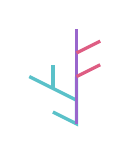
\begin{tikzpicture}[scale=0.3, very thick]
\draw[bleu] (-1,0.5)--(0,0)--(0,2);
\draw[bleu] (0,1)--(-2,2);
\draw[bleu] (-1,1.5)--(-1,2.5);
\draw[mauve](0,0)--(0,4);
\draw[rose](0,3)--(1,3.5);
\draw[rose](0,2)--(1,2.5);
\end{tikzpicture} \! & \raisebox{0.5cm}{$+$} &

\begin{tikzpicture}[scale=0.3, very thick]
\draw[bleu] (-1,0.5)--(0,0)--(0,2);
\draw[bleu] (0,1)--(-2,2);
\draw[bleu] (-1,1.5)--(-1,2.5);
\draw[mauve](0,0)--(0,3);
\draw[rose](0,1)--(1,1.5);
\draw[rose](0,2)--(1,2.5);
\end{tikzpicture}& \raisebox{0.5cm}{$+$} & 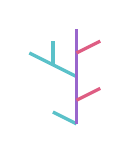
\begin{tikzpicture}[scale=0.3, very thick]
\draw[bleu] (-1,0.5)--(0,0);
\draw[bleu] (0,2)--(-2,3);
\draw[bleu] (-1,2.5)--(-1,3.5);
\draw[mauve](0,0)--(0,4);
\draw[rose](0,3)--(1,3.5);
\draw[rose](0,1)--(1,1.5);
\end{tikzpicture}  & \raisebox{0.5cm}{$+$} & 
\begin{tikzpicture}[scale=0.3, very thick]
\draw[bleu] (-1,0.5)--(0,0);
\draw[bleu] (0,2)--(-2,3);
\draw[bleu] (-1,2.5)--(-1,3.5);
\draw[mauve](0,0)--(0,3);
\draw[rose](0,2)--(1,2.5);
\draw[rose](0,1)--(1,1.5);
\end{tikzpicture} & \raisebox{0.5cm}{$+$} & 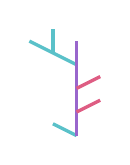
\begin{tikzpicture}[scale=0.3, very thick]
\draw[bleu] (-1,0.5)--(0,0);
\draw[bleu] (0,3)--(-2,4);
\draw[bleu] (-1,3.5)--(-1,4.5);
\draw[mauve](0,0)--(0,4);
\draw[rose](0,2)--(1,2.5);
\draw[rose](0,1)--(1,1.5);
\end{tikzpicture} & \raisebox{0.5cm}{$+$} & 
\begin{tikzpicture}[scale=0.3, very thick]
\draw[bleu] (-1,1.5)--(0,1);
\draw[bleu] (0,2)--(-2,3);
\draw[bleu] (-1,2.5)--(-1,3.5);
\draw[mauve](0,1)--(0,4);
\draw[rose](0,3)--(1,3.5);
\draw[rose](0,1)--(1,1.5);
\end{tikzpicture} & \raisebox{0.5cm}{$+$} &
 \\
&& 
\begin{tikzpicture}[scale=0.3, very thick]
\draw[bleu] (-1,1.5)--(0,1);
\draw[bleu] (0,2)--(-2,3);
\draw[bleu] (-1,2.5)--(-1,3.5);
\draw[mauve](0,1)--(0,3);
\draw[rose](0,2)--(1,2.5);
\draw[rose](0,1)--(1,1.5);
\end{tikzpicture} & \raisebox{0.5cm}{$+$} &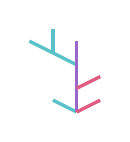
\begin{tikzpicture}[scale=0.3, very thick]
\draw[bleu] (-1,1.5)--(0,1);
\draw[bleu] (0,3)--(-2,4);
\draw[bleu] (-1,3.5)--(-1,4.5);
\draw[mauve](0,1)--(0,4);
\draw[rose](0,2)--(1,2.5);
\draw[rose](0,1)--(1,1.5);
\end{tikzpicture} & \raisebox{0.5cm}{$+$} & 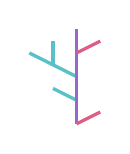
\begin{tikzpicture}[scale=0.3, very thick]
\draw[bleu] (-1,1.5)--(0,1);
\draw[bleu] (0,2)--(-2,3);
\draw[bleu] (-1,2.5)--(-1,3.5);
\draw[mauve](0,0)--(0,4);
\draw[rose](0,3)--(1,3.5);
\draw[rose](0,0)--(1,0.5);
\end{tikzpicture} & \raisebox{0.5cm}{$+$} & 
\begin{tikzpicture}[scale=0.3, very thick]
\draw[bleu] (-1,1.5)--(0,1);
\draw[bleu] (0,2)--(-2,3);
\draw[bleu] (-1,2.5)--(-1,3.5);
\draw[mauve](0,0)--(0,3);
\draw[rose](0,2)--(1,2.5);
\draw[rose](0,0)--(1,0.5);
\end{tikzpicture} & \raisebox{0.5cm}{$+$} & 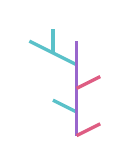
\begin{tikzpicture}[scale=0.3, very thick]
\draw[bleu] (-1,1.5)--(0,1);
\draw[bleu] (0,3)--(-2,4);
\draw[bleu] (-1,3.5)--(-1,4.5);
\draw[mauve](0,0)--(0,4);
\draw[rose](0,2)--(1,2.5);
\draw[rose](0,0)--(1,0.5);
\end{tikzpicture} & \raisebox{0.5cm}{$+$} & 
\begin{tikzpicture}[scale=0.3, very thick]
\draw[bleu] (-1,1.5)--(0,1);
\draw[bleu] (0,2)--(-2,3);
\draw[bleu] (-1,2.5)--(-1,3.5);
\draw[mauve](0,0)--(0,3);
\draw[rose](0,1)--(1,1.5);
\draw[rose](0,0)--(1,0.5);
\end{tikzpicture} & \raisebox{0.5cm}{$+$} & 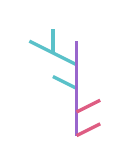
\begin{tikzpicture}[scale=0.3, very thick]
\draw[bleu] (-1,2.5)--(0,2);
\draw[bleu] (0,3)--(-2,4);
\draw[bleu] (-1,3.5)--(-1,4.5);
\draw[mauve](0,0)--(0,4);
\draw[rose](0,1)--(1,1.5);
\draw[rose](0,0)--(1,0.5);
\end{tikzpicture} \\[0.4cm] 
& \raisebox{0.5cm}{$=$} &

\begin{tikzpicture}[scale=0.27, very thick]
\draw[bleu] (-1,1)--(0,0)--(2,2);
\draw[bleu] (1,1)--(0,2)--(-0.8,3);
\draw[bleu] (0,2)--(0.8,3);
\draw[rose](0.4,4)--(2,2)--(2.8,3);
\draw[rose](1.2,3)--(2,4);
\end{tikzpicture} & \raisebox{0.5cm}{$+$} &

\begin{tikzpicture}[scale=0.3, very thick]
\draw[bleu] (-1,1)--(0,0)--(1,1);
\draw[bleu] (1,1)--(-0.5,2)--(-1,3);
\draw[bleu] (-0.5,2)--(0,3);
\draw[rose](0.5,3)--(1,2)--(1.5,3);
\draw[rose](1,1)--(2,2);
\draw[mauve] (1,2)--(1,1);
\end{tikzpicture} & \raisebox{0.5cm}{$+$} &

\begin{tikzpicture}[scale=0.27, very thick]
\draw[bleu] (-1,1)--(0,0)--(1,1);
\draw[rose](0,2)--(1,1)--(2,2);
\draw[bleu] (-1,3)--(0,2)--(1,3);
\draw[bleu] (-1.8,4)--(-1,3)--(-0.2,4);
\draw[rose](0.2,4)--(1,3)--(1.8,4);
\end{tikzpicture} & \raisebox{0.5cm}{$+$} &

\begin{tikzpicture}[scale=0.3, very thick]
\draw[bleu] (0,0)--(1,-1)--(2,0);
\draw[bleu] (1,1)--(-0.5,2)--(-1,3);
\draw[bleu] (-0.5,2)--(0,3);
\draw[rose](1,1)--(2,0)--(3,1);
\draw[rose](1,1)--(2,2);
\draw[mauve] (1,2)--(1,1);
\end{tikzpicture}
& \raisebox{0.5cm}{$+$} &

\begin{tikzpicture}[scale=0.25, very thick]
\draw[bleu] (-1,1)--(0,0)--(1,1);
\draw[rose](-1,3)--(1,1)--(2,2);
\draw[rose] (0,2)--(1,3);
\draw[bleu] (-2,4)--(-1,3)--(0,4);
\draw[bleu] (-2.8,5)--(-2,4)--(-1.2,5);
\end{tikzpicture}
& \raisebox{0.5cm}{$+$} &

\begin{tikzpicture}[scale=0.3, very thick]
\draw[bleu] (-1,1)--(0,0);
\draw[mauve] (0,0)--(0,1);
\draw[rose](0,0)--(1,1);
\draw[bleu] (-1,2)--(0,1)--(1,2);
\draw[bleu] (-1.8,3)--(-1,2)--(-0.2,3);
\draw[rose] (0.2,3)--(1,2)--(1.8,3);
\end{tikzpicture} 
& \raisebox{0.5cm}{$+$} & \\[0.2cm]
&& 
\begin{tikzpicture}[scale=0.3, very thick]
\draw[bleu] (-1,1)--(0,0);
\draw[mauve] (0,0)--(0,1);
\draw[rose](0,0)--(1,1);
\draw[bleu] (-1,2)--(0,1);
\draw[mauve] (0,1)--(0,2);
\draw[rose](0,1)--(1,2);
\draw[bleu] (-2,3)--(-1,2)--(0,3);
\end{tikzpicture}& \raisebox{0.5cm}{$+$} &

\begin{tikzpicture}[scale=0.3, very thick]
\draw[bleu] (-1,1)--(0,0);
\draw[mauve] (0,0)--(0,1);
\draw[rose](0,0)--(1,1);
\draw[rose](-1,2)--(0,1)--(1,2);
\draw[bleu] (-2,3)--(-1,2)--(0,3);
\draw[bleu] (-3,4)--(-2,3)--(-1,4);
\end{tikzpicture}& \raisebox{0.5cm}{$+$} &

\begin{tikzpicture}[scale=0.25, very thick]
\draw[rose] (-1,1)--(0,0)--(1,1);
\draw[bleu](-2,2)--(-1,1)--(1,3);
\draw[rose] (0.2,4)--(1,3)--(1.8,4);
\draw[bleu] (0,2)--(-1,3)--(-1.8,4);
\draw[bleu] (-1,3)--(-0.2,4);
\end{tikzpicture}& \raisebox{0.5cm}{$+$} &

\begin{tikzpicture}[scale=0.27, very thick]
\draw[rose] (-1,1)--(0,0)--(1,1);
\draw[bleu](-2,2)--(-1,1)--(0,2);
\draw[rose] (0,2)--(1,3);
\draw[mauve] (0,2)--(0,3);
\draw[bleu] (0,2)--(-1,3)--(-1.8,4);
\draw[bleu] (-1,3)--(-0.2,4);
\end{tikzpicture}& \raisebox{0.5cm}{$+$} &

\begin{tikzpicture}[scale=0.25, very thick]
\draw[rose] (-1,1)--(0,0)--(1,1);
\draw[bleu](-2,2)--(-1,1)--(0,2);
\draw[rose] (-1,3)--(0,2)--(1,3);
\draw[bleu] (0,4)--(-1,3)--(-2,4)--(-2.8,5);
\draw[bleu] (-1.2,5)--(-2,4);
\end{tikzpicture}& \raisebox{0.5cm}{$+$} &

\begin{tikzpicture}[scale=0.27, very thick]
\draw[rose] (-1,1)--(0,0)--(1,1);
\draw[bleu](-2,2)--(-1,1);
\draw[mauve](-1,1)--(-1,2);
\draw[rose] (-1,1)--(0,2);
\draw[bleu] (-2,3)--(-1,2)--(0,3);
\draw[bleu] (-3,4)--(-2,3)--(-1,4);
\end{tikzpicture} & \raisebox{0.5cm}{$+$} &

\begin{tikzpicture}[scale=0.25, very thick]
\draw[rose](0,0)--(2,-2)--(3,-1);
\draw[rose](1,-1)--(2,0);
\draw[bleu] (-1,1)--(0,0)--(2,2);
\draw[bleu] (1,1)--(0,2)--(-0.8,3);
\draw[bleu] (0,2)--(0.8,3);
\end{tikzpicture}\end{tabular}}\endgroup\end{center} 
is split into
\begin{center}
\resizebox{9.5cm}{!}{\begin{tabular}{rcl}
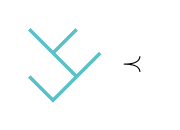
\begin{tikzpicture}[scale=0.3,color=bleu, very thick]
\draw (-1,1)--(0,0)--(2,2);
\draw (1,1)--(-1,3);
\draw (0,2)--(1,3);
\draw[black, very thick] (3.35,1.5) node{$\prec$};
\end{tikzpicture}

\begin{tikzpicture}[scale=0.3,color=rose, very thick]
\draw (-2,2)--(0,0)--(1,1);
\draw (-1,1)--(0,2);
\end{tikzpicture} & \raisebox{0.4cm}{=} &

\begin{tikzpicture}[scale=0.27, very thick]
\draw[bleu] (-1,1)--(0,0)--(2,2);
\draw[bleu] (1,1)--(0,2)--(-0.8,3);
\draw[bleu] (0,2)--(0.8,3);
\draw[rose](0.4,4)--(2,2)--(2.8,3);
\draw[rose](1.2,3)--(2,4);
\end{tikzpicture}\,\,\raisebox{0.4cm}{+}\,\,

\begin{tikzpicture}[scale=0.3, very thick]
\draw[bleu] (-1,1)--(0,0)--(1,1);
\draw[bleu] (1,1)--(-0.5,2)--(-1,3);
\draw[bleu] (-0.5,2)--(0,3);
\draw[rose](0.5,3)--(1,2)--(1.5,3);
\draw[rose](1,1)--(2,2);
\draw[mauve] (1,2)--(1,1);
\end{tikzpicture}\,\,\,\raisebox{0.4cm}{+}  

\begin{tikzpicture}[scale=0.27, very thick] 
\draw[bleu] (-1,1)--(0,0)--(1,1);
\draw[rose](0,2)--(1,1)--(2,2);
\draw[bleu] (-1,3)--(0,2)--(1,3);
\draw[bleu] (-1.8,4)--(-1,3)--(-0.2,4);
\draw[rose](0.2,4)--(1,3)--(1.8,4);
\end{tikzpicture}\,\,\,\raisebox{0.4cm}{+}  

\begin{tikzpicture}[scale=0.3, very thick]

\draw[bleu] (0,0)--(1,-1)--(2,0);
\draw[bleu] (1,1)--(-0.5,2)--(-1,3);
\draw[bleu] (-0.5,2)--(0,3);
\draw[rose](1,1)--(2,0)--(3,1);
\draw[rose](1,1)--(2,2);
\draw[mauve] (1,2)--(1,1);
\end{tikzpicture}\,\,\,\raisebox{0.4cm}{+}  

\begin{tikzpicture}[scale=0.25, very thick]
\draw[bleu] (-1,1)--(0,0)--(1,1);
\draw[rose](-1,3)--(1,1)--(2,2);
\draw[rose] (0,2)--(1,3);
\draw[bleu] (-2,4)--(-1,3)--(0,4);
\draw[bleu] (-2.8,5)--(-2,4)--(-1.2,5);
\end{tikzpicture} \\ 



\begin{tikzpicture}[scale=0.3,color=bleu, very thick]
\draw (-1,1)--(0,0)--(2,2);
\draw (1,1)--(-1,3);
\draw (0,2)--(1,3);
\draw[black, very thick] (3.35,1.5) node{$\bcdot$};
\end{tikzpicture}\!

\begin{tikzpicture}[scale=0.3,color=rose, very thick]
\draw (-2,2)--(0,0)--(1,1);
\draw (-1,1)--(0,2); 
\end{tikzpicture}  &\raisebox{0.4cm}{=}  &

\begin{tikzpicture}[scale=0.3, very thick]
\draw[bleu] (-1,1)--(0,0);
\draw[mauve] (0,0)--(0,1);
\draw[rose](0,0)--(1,1);
\draw[bleu] (-1,2)--(0,1)--(1,2);
\draw[bleu] (-1.8,3)--(-1,2)--(-0.2,3);
\draw[rose] (0.2,3)--(1,2)--(1.8,3);
\end{tikzpicture}\,\,\,\raisebox{0.4cm}{+}  

\begin{tikzpicture}[scale=0.3, very thick]
\draw[bleu] (-1,1)--(0,0);
\draw[mauve] (0,0)--(0,1);
\draw[rose](0,0)--(1,1);
\draw[bleu] (-1,2)--(0,1);
\draw[mauve] (0,1)--(0,2);
\draw[rose](0,1)--(1,2);
\draw[bleu] (-2,3)--(-1,2)--(0,3);
\end{tikzpicture}\,\,\,\raisebox{0.4cm}{+}  

\begin{tikzpicture}[scale=0.3, very thick]
\draw[bleu] (-1,1)--(0,0);
\draw[mauve] (0,0)--(0,1);
\draw[rose](0,0)--(1,1);
\draw[rose](-1,2)--(0,1)--(1,2);
\draw[bleu] (-2,3)--(-1,2)--(0,3);
\draw[bleu] (-3,4)--(-2,3)--(-1,4);
\end{tikzpicture}\\ 


\begin{tikzpicture}[scale=0.3,color=bleu, very thick]
\draw (-1,1)--(0,0)--(2,2);
\draw (1,1)--(-1,3);
\draw (0,2)--(1,3);
\draw[black, very thick] (3.5,1.5) node{$\succ$};
\end{tikzpicture}

\begin{tikzpicture}[scale=0.3,color=rose, very thick]
\draw (-2,2)--(0,0)--(1,1);
\draw (-1,1)--(0,2);
\end{tikzpicture} & \raisebox{0.4cm}{=} &

\begin{tikzpicture}[scale=0.25, very thick]
\draw[rose] (-1,1)--(0,0)--(1,1);
\draw[bleu](-2,2)--(-1,1)--(1,3);
\draw[rose] (0.2,4)--(1,3)--(1.8,4);
\draw[bleu] (0,2)--(-1,3)--(-1.8,4);
\draw[bleu] (-1,3)--(-0.2,4);
\end{tikzpicture}\,\,\,\raisebox{0.4cm}{+}  \,\,

\begin{tikzpicture}[scale=0.27, very thick]
\draw[rose] (-1,1)--(0,0)--(1,1);
\draw[bleu](-2,2)--(-1,1)--(0,2);
\draw[rose] (0,2)--(1,3);
\draw[mauve] (0,2)--(0,3);
\draw[bleu] (0,2)--(-1,3)--(-1.8,4);
\draw[bleu] (-1,3)--(-0.2,4);
\end{tikzpicture}\,\,\,\raisebox{0.4cm}{+}  

\begin{tikzpicture}[scale=0.25, very thick]
\draw[rose] (-1,1)--(0,0)--(1,1);
\draw[bleu](-2,2)--(-1,1)--(0,2);
\draw[rose] (-1,3)--(0,2)--(1,3);
\draw[bleu] (0,4)--(-1,3)--(-2,4)--(-2.8,5);
\draw[bleu] (-1.2,5)--(-2,4);
\end{tikzpicture}\,\,\,\raisebox{0.4cm}{+}  

\begin{tikzpicture}[scale=0.27, very thick]
\draw[rose] (-1,1)--(0,0)--(1,1);
\draw[bleu](-2,2)--(-1,1);
\draw[mauve](-1,1)--(-1,2);
\draw[rose] (-1,1)--(0,2);
\draw[bleu] (-2,3)--(-1,2)--(0,3);
\draw[bleu] (-3,4)--(-2,3)--(-1,4);
\end{tikzpicture}\,\,\,\raisebox{0.4cm}{+}  

\begin{tikzpicture}[scale=0.25, very thick]
\draw[rose](0,0)--(2,-2)--(3,-1);
\draw[rose](1,-1)--(2,0);
\draw[bleu] (-1,1)--(0,0)--(2,2);
\draw[bleu] (1,1)--(0,2)--(-0.8,3);
\draw[bleu] (0,2)--(0.8,3);
\end{tikzpicture}\end{tabular}}
\end{center}

Burgunder and Ronco  applied a similar  ternary splitting to surjections, also known as packed words, and obtained also a tridendriform structure.


Associahedra and permutohedra are instances of polytopes called \emph{hypergraph polytopes}
 \cite{DP}, which are obtained by truncating some faces of simplices, and are also known as \emph{nestohedra} \cite{P09}. The description of faces of hypergraph polytopes in terms of tree structures -- called constructs -- used as working definition in \cite{COI}  provides an adapted framework to extend the setting of Loday--Ronco and Burgunder--Ronco to other families  of polytopes. 

We find it convenient to work in an  ``unbiased'' setting, where our operations may have any finite arity (think of the product $a\times b\times c$ of three numbers $a,b,c$ as opposed to $(a \times b)\times c$ or $a\times (b\times c)$). This leads us to a reformulation of the tridendriform  (actually $q$-tridendriform  -- see below) structure, that we call polydendriform.  We exhibit conditions under which we can define such a polydendriform structure.

The underlying (binary) associative product that we obtain specializes to the associative product defined by Ronco \cite{RoncoGTO} in the setting of graph associahedra \cite{CD-CCGA}, which are the hypergraph polytopes where the associated hypergraphs have only hyperedges of cardinality at most two (see Remark \ref{Ronco-specialize}). Our results apply also  to some families of hypergraph polytopes that are not graph associahedra, such as simplices, hypercubes and erosohedra.
 
 Therefore, with respect to  \cite{RoncoGTO}, our extension is two-fold:  we describe not only an associative product, but also a tridendriform splitting of it, and our framework applies in situations that are not covered there.

The article is organized as follows. 
In  \S\ref{Prologue-section}, we explain in detail the case of the permutohedra,
and motivate and recall Burgunder--Ronco's notion of $q$-tridendriform algebra, i.e.  an algebra with operations ``$\prec$'', ``$\succ$'' and ``$\bcdot$'',  satisfying the same equations as in tridendriform algebras, but with the associated (associative) product being now defined as $\ast = (\prec) + (\succ) + q( \bcdot)$  for an arbitrary $q \in \mathbb{K}$, where $\mathbb{K}$ is the ambient field.
In \S\ref{reminders-hypergraph-section}, we recall some notions on hypergraph polytopes and constructs.
In \S\ref{strict-teams}, we introduce our conditions for  the set of faces of a family of polytopes to be endowed with a polydendriform algebra structure. We first give a so-called ``strict'' condition  that makes it possible to define $q$-tridendriform algebras, for arbitrary $q$. We then give a weaker condition called ``quasi-strict'', which allows us to deal with a wider class of examples, but for which $q$ has to be $-1$.  In \S\ref{reminders-hypergraph-section} and \S\ref{strict-teams}, we provide a bunch of new examples that do not fit in the framework of graph associahedra, such as simplices, hypercubes and a family that we call erosohedra. We also introduce a family of graph associahedra that we call friezohedra and will serve as a running example throughout the paper.

\paragraph{\bf Warning.}
We  would like to mention the existence of the terms ``polydendriform'' \cite{Samuele} and ``hypergraphic polytope'' \cite{AguiarArdila} 
in the literature, which designate different concepts from the ones presented in this article.


\section{Prologue} \label{Prologue-section}

We recall Burgunder--Ronco's shuffle product on the faces of permutohedra~\cite{BR}.
We set $[n]=\set{1,\ldots,n}$, and identify a function $f:[n]\rightarrow X$ (for some set $X$) with the sequence $(f(1),\ldots,f(n))$.

By {\em surjection}, we mean a function $f:[m]\rightarrow[n]$ (for some $m,n\geq 1$) that is surjective.  
For arbitrary $h:[m]\rightarrow[n]$, we can build a surjection 
${\tt pack}(h):=\phi\circ h: [m]\rightarrow [|{\tt Im}(h)|]$,
where $\phi$ is the unique increasing bijection ${\tt Im}(h)\rightarrow  [|{\tt Im}(h)|]$.
For example, we have
 ${\tt pack}(1,4,3,4)=(1,3,2,3)$. Surjections label the faces of permutohedra, as shown by Chapoton in \cite{Ch00}. Surjections also appear in  \cite{HNT} under the name of {\em packed words}   as building blocks of the Hopf algebra {\bf WQSym}, isomorphic to the one defined for permutohedra by Chapoton.  The computations we make below in Burgunder--Ronco style correspond precisely to the computations and the tridendriform decomposition in {\bf WQSym} as described in \cite{HNT}.
 
If $f:[m_1]\rightarrow[n_1]$ and $g:[m_2]\rightarrow[n_2]$ are surjections, we look for 
 all surjections $(h,k):[m_1+m_2]\rightarrow [n]$, for $\max(n_1,n_2)\leq n\leq n_1+n_2$,  such that
 ${\tt pack}(h)=f$ and ${\tt pack}(k)=g$.  Below, we do this for 
$f:=(1,2,1)$ and $g:=(2,1)$, underlining the maximum elements  of $h$ and of $k$.
\begin{itemize}
\item {\small $n=2$:   $(1,\ul{2},1,\ul{2},1)$}
\item {\small $n=3$: $(1,\ul{2},1,\ul{3},1)$, $(1,\ul{3},1,\ul{3},2)$, $(2,\ul{3},2,\ul{2},1)$, $(1,\ul{2},1,\ul{3},2)$,  $(1,\ul{3},1,\ul{2},1)$,  $(2,\ul{3},2,\ul{3},1)$}
\item {\small $n=4$:
$(1,\ul{2},1,\ul{4},3)$, $(1,\ul{3},1,\ul{4},2)$,  $(1,\ul{4},1,\ul{3},2)$,  $(2,\ul{3},2,\ul{4},1)$, $(2,\ul{4},2,\ul{3},1)$, $(3,\ul{4},3,\ul{2},1)$.}
\end{itemize}
We collect those pairs in the following formal sums (cf. \S\ref{Intro-section}): 
{\small{$$\begin{array}{lll}
 f\prec g&  := & {(2,\ul{3},2,\ul{2},1)} 
 +  {(1,\ul{3},1,\ul{2},1)} 
 +  {(1,\ul{4},1,\ul{3},2)} 
 +  {(2,\ul{4},2,\ul{3},1)} 
 +  (3,\ul{4},3,\ul{2},1)  \\
 && \mathit{(\max(h)>\max(k))}\\
  f\bcdot g & := &  {(1,\ul{2},1,\ul{2},1)} +  {(1,\ul{3},1,\ul{3},2)} + { (2,\ul{3},2,\ul{3},1)} \\
  && \mathit{(\max(h)=\max(k))}\\
  {  f\succ g}&  := &  {  (1,\ul{2},1,\ul{3},1)} 
  +  {  (1,\ul{2},1,\ul{3},2)}
  +  {  (1,\ul{2},1,\ul{4},3)}   +  {  (1,\ul{3},1,\ul{4},2)}
    +   {  (2,\ul{3},2,\ul{4},1)} \\
   & &\mathit{(\max(h)<\max(k))}\\
  f\ast g&  := & ({  f\prec g}) + ({  f\bcdot g}) + ({ f\succ g}).
\end{array}$$}}
\normalsize
   The operations $\prec$, $\bcdot$ and $\succ$ satisfy the following {\em tridendriform} equations
$$\begin{array}{lr}
 (a\prec b)\prec c=a\prec(b\ast c) & \quad\quad\quad\mathit{(\precstar)} \\
 (a\succ b)\prec c=a\succ(b\prec c) & \mathit{(\succ\prec)} \\
 (a\ast b)\succ c=a\succ(b\succ c) & \mathit{(\astsucc)} \\
(a\bcdot b)\bcdot c=a\bcdot(b\bcdot c) & \mathit{(\bcdotass)} \\
 (a\succ b)\bcdot c=a\succ(b\bcdot c) & \mathit{(\succbcdot)}  \\
 (a\prec b)\bcdot c=a\bcdot (b\succ c) & \mathit{(\precbcdotsucc)} \\ 
(a\bcdot b)\prec c=a\bcdot (b\prec c) & \mathit{(\bcdotprec)} \\
\end{array}$$
  and  the operation $\ast$ is associative.

The tridendriform structure was first recognized and defined by Loday and Ronco~\cite{LR} on Schr\"oder trees, i.e. planar trees without  unary nodes. We will denote such trees as $\bullet(T_1,\ldots,T_n)$, for $n\neq 1$, where $T_1, \ldots, T_n$ are themselves Schr\"oder trees. The tree with only one leaf is then $\bullet()$.
Schr\"oder trees with at least two leaves label the faces of associahedra.
The three tridendriform operations  (already illustrated in \S\ref{Intro-section}) are defined as follows (with the convention that $\bullet() \ast S=S=S\ast\bullet()$):
$$\begin{array}{rcl}
\bullet(S_1,\ldots,S_n)\prec T & :=& \bullet (S_1,\ldots,S_{n-1},S_n\ast T)\\
S\succ \bullet (T_1,\ldots,T_n) & := & \bullet(S\ast T_1,T_2,\ldots,T_n) \\
\bullet(S_1,\ldots,S_m) \:\bcdot\: \bullet(T_1,\ldots,T_n) & := & \bullet(S_1,\ldots,S_{m-1}, S_m\ast T_1,T_2\ldots,T_n) .
\end{array}$$

Associahedra and permutohedra are examples of hypergraph polytopes, also known as nestohedra \cite{P09,FS05}. Our goal is to define in this more general framework, and under suitable conditions, an associative product, with associated tridendriform decomposition, instantiating to these two examples and  more.

We close this section by studying the relation between tridendriform structures and associativity more closely.  Burgunder and Ronco~\cite{BR} have introduced a variation of tridendriform algebras, called $q$-tridendriform  algebras (for $q\in \mathbb{R}$, or more generally $q\in {\Bbbk}$ for some field ${\Bbbk}$), where the equations are the same as above, except that now the operation $\bcdot$ is weighted, i.e. $a\ast b$ is redefined as $(a\prec b)+q(a\bcdot b)+(a\succ b)$. This is justified by the following proposition.
\begin{proposition} \label{tridend-implies-ass}
Setting $a\ast b:=\lambda_1(a\prec b)+\lambda_2(a\bcdot b)+\lambda_3(a\succ b)$, if the tridendriform equations are satisfied (with this definition of $\ast$), then $\ast$ is associative if  $\lambda_1=\lambda_3=1$.
\end{proposition} 
\begin{proof} We match
 $$\begin{array}{ll}
 \lambda_1\lambda_1 \underbrace{ (a\prec b)\prec c}_{(\precstar)} \:+\: \lambda_1\lambda_2\underbrace{(a\bcdot b)\prec c}_{(\bcdotprec)} \:+\: \lambda_1\lambda_3 
\underbrace{(a\succ b)\prec c}_{(\succ\prec)}  \:+\: \lambda_2\lambda_1 \underbrace{(a\prec b)\bcdot c}_{(\precbcdotsucc)} \\
 \:+\: \lambda_2\lambda_2 \underbrace{(a\bcdot b)\bcdot c}_{(\bcdotass)}
\:+\: \lambda_2\lambda_3 \underbrace{(a\succ b)\bcdot c}_{(\succbcdot)}  \:+\: \lambda_3\underbrace{ (a\ast b)\succ c}_{(\astsucc)}
 \end{array}$$
 with
 $$\begin{array}{ll}
 \lambda_1 \underbrace{a\prec (b\ast c)}_{(\precstar)}  \:+\:
\lambda_2 \lambda_1 \underbrace{ a\bcdot (b\prec c)}_{(\bcdotprec)} \:+\: \lambda_2\lambda_2 \underbrace{a\bcdot (b\bcdot c)}_{(\bcdotass)}  \:+\: \lambda_2\underbrace{\lambda_3 a\bcdot (b\succ c)}_{(\precbcdotsucc)} \\ 
 \:+\: \lambda_3\lambda_1 \underbrace{a\succ(b\prec c)}_{(\succ\prec)} \:+\: \lambda_3\lambda_2 \underbrace{a\succ(b\bcdot c)}_{(\succbcdot)} \:+\:
\lambda_3\lambda_3 \underbrace{a\succ(b\succ c)}_{(\astsucc)}
\end{array}$$
 using $(\precstar)$ (resp. $(\astsucc)$, $(\precbcdotsucc)$) and the assumption $\lambda_1=1$ (resp.  $\lambda_1 = \lambda_3=1$).
\end{proof}
\section{Hypergraph polytopes} \label{reminders-hypergraph-section}

We first recall all the needed definitions in \S\ref{basic-definitions-section}, and then give a number of examples in \S\ref{notable-section}.

\subsection{Basic definitions} \label{basic-definitions-section}
A hypergraph is given by a set  $H$ of vertices (the carrier), and a subset 
$\hyper{H}\inc {\mathcal{P}}(H)\backslash\emptyset$ such that $\Union \hyper{H}=H$.
 The elements of $\hyper{H}$ are called the {\em hyperedges} of $\hyper{H}$.  
 We always assume that $\hyper{H}$ is {\em atomic}, by which we mean that 
 $\set{x}\in \hyper{H}$, for all $x\in H$. 
 Identifying $x$ with $\set{x}$, $H$ can be seen as the set of  hyperedges of 
 cardinality $1$, also called {\em vertices}. We shall use the convention to 
 give the same name to the hypergraph and to its carrier, the former being 
 the bold version of the latter. 
A hyperedge of cardinality 2 is called an {\em edge}.  Note that any ordinary graph $(V,E)$ can be viewed as the atomic hypergraph
$\setc{\set{v}}{v\in V} \union \setc{e}{e\in E}$ (with no hyperedges of cardinality $\geq 3$). 

If $\hyper{H}$ is a hypergraph,  and if  $X\inc H$, we set
$\hyper{H}_X:=\setc{Z}{Z\in \hyper{H}\;\mbox{and}\; Z\inc X}$, and $\restrH{H}{X}=\hyper{H}_{H\backslash X}$.
We say that $\hyper{H}$ is {\em connected} if there is no non-trivial partition $H=X_1\union X_2$ such that $\hyper{H}=\hyper{H}_{X_1}\union \hyper{H}_{X_2}$, and that $X\inc H$ is connected in $\hyper{H}$, or that $X$ is a {\em tube} \footnote{The name ``tube'' was originally introduced in the setting of graphs and graph associahedra \cite{CD-CCGA}. We extend here its use to hypergraphs.}
of  $\hyper{H}$, if $\hyper{H}_X$ is connected.
For each finite hypergraph there exists a unique partition
$H=X_1\union\ldots\union X_m$ such that each $\hyper{H}_{X_i}$ is connected and $\hyper{H}=\Union(\hyper{H}_{X_i})$.  The $\hyper{H}_{X_i}$ are  the {\em connected components} of $\hyper{H}$. The notation
$\hyper{H},X  \leadsto \hyper{H}_1,\ldots, \hyper{H}_n$
 will mean that  $\hyper{H}_1,\ldots,\hyper{H}_n$ are  the
 connected components of $\restrH{H}{X}$.  

Do\v sen and Petri\'c~\cite{DP} have proposed the following insightful reading of the data of a finite connected hypergraph $\hyper{H}$ as a truncated simplex: the elements of $H$ are identified with the facets (i.e. codimension 1 faces) of the $(|H|-1)$-dimensional simplex, and each $\emptyset\incs X\incs H$, $|X|\geq 2$, such that    $\hyper{H}_X$ is connected designates the intersection of the facets in $X$ as a face to be truncated. The obtained polytopes, called \emph{hypergraph polytopes}, extend the construction of graph associahedra \cite{CD-CCGA, Zel06}, and are equivalent to nestohedra.

\begin{example}\label{hypergraphex1} The hypergraph 
 $${\bf H}=\{\{x\},\{y\},\{u\},\{v\},\{x,y\},\{x,u\},\{x,v\},\{u,v\},\{x,u,v\}\}$$    can be represented pictorially as follows:
\begin{center}
\resizebox{2cm}{!}{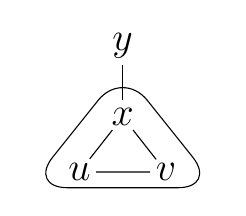
\begin{tikzpicture}
\node (x) [circle,draw=none,inner sep=0.2mm,minimum size=1mm] at (1,0.9) {\Large $x$};
\node (y) [circle,draw=none,inner sep=0.2mm,minimum size=1mm] at (1,1.8) {\Large $y$};
\node (u) [circle,draw=none,inner sep=0.2mm,minimum size=1mm]at (0.45,0.2) {\Large $u$};
\node (v) [circle,draw=none,inner sep=0.2mm,minimum size=1mm] at (1.55,0.2) {\Large $v$};
\draw [rounded corners=5mm,fill=none] (1,1.5)--(-0.2,0)--(2.2,0)--cycle;
\draw (x)--(u)--(v)--(x);\draw (x)--(y);
\end{tikzpicture}}
\end{center}
Here, the hyperedge $\{x,u,v\}$ is represented by the circled-out  area around the vertices $x$, $u$ and $v$. We show in Figure \ref{hemiassoc} the polytope encoded by  ${\bf H}$. \demo

 \end{example}
\begin{figure}
\centering
  \resizebox{5.5cm}{!}{
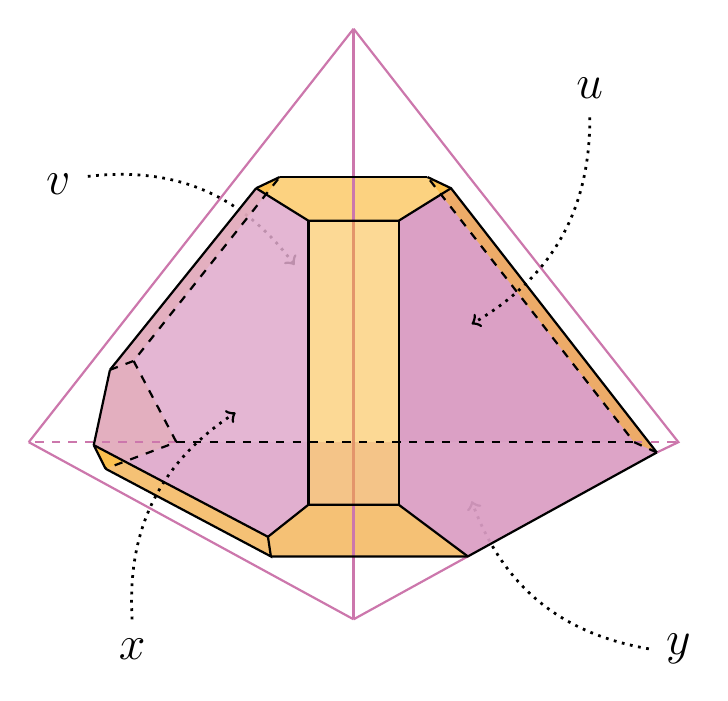
\begin{tikzpicture}[thick,scale=3.75]
\draw (-0.9,1.5) edge[->,dotted, bend left, line width=1pt] (-0.2,1.2);
\draw (1,-0.1) edge[->,dotted, bend left, line width=1pt] (0.4,0.4);
\node at (1.1,-0.1) {\LARGE $y$};
\node at (-1,1.475) {\LARGE $v$};
\coordinate (A1) at (0,2);
\coordinate (A11) at (-0.39,1.5);
\coordinate (A111) at (-0.25,1.498);
\coordinate (A112) at (-0.33,1.46);
\coordinate (A12) at (0.39,1.5);
\coordinate (A121) at (0.25,1.498);
\coordinate (A122) at (0.33,1.46);
\coordinate (A13) at (0,1.25);
\coordinate (A131) at (-0.153,1.35); 
\coordinate (A132) at (0.153,1.35); 
\coordinate (A2) at (0,0); 
\coordinate (A21) at (-0.387,0.213); 
\coordinate (A211) at (-0.29,0.2795); 
\coordinate (A212) at (-0.28,0.213); 
\coordinate (A22) at (0.387,0.213); 
\coordinate (A23) at (0,0.5); 
\coordinate (A231) at (-0.153,0.388); 
\coordinate (A232) at (0.153,0.388); 
\coordinate (A3) at (-1.1,0.6);
\coordinate (A31) at (-0.9,0.49);
\coordinate (A311) at (-0.88,0.59);
\coordinate (A312) at (-0.84,0.51);
\coordinate (A32) at (-0.8,0.976);
\coordinate (A321) at (-0.825,0.845);
\coordinate (A322) at (-0.745,0.875);
\coordinate (A33) at (-0.6,0.6);
\coordinate (A4) at (1.1,0.6);
\coordinate (A41) at (1.027,0.565);
\coordinate (A42) at (0.95,0.6);
\fill [fill=Dandelion,fill opacity=0.6] (A321)--(A322)--(A111)--(A112)--cycle;
\fill [fill=Dandelion,fill opacity=0.6] (A312)--(A311)--(A321)--(A322)--(A33)--cycle;
\fill [fill=RedViolet!30,fill opacity=0.85] (A112)--(A131)--(A231)--(A211)--(A311)--(A321)--cycle;
\fill [fill=Dandelion,fill opacity=0.6] (A112)--(A111)--(A121)--(A122)--(A132)--(A131)--cycle;
\fill [fill=RedViolet!40,fill opacity=0.85] (A132)--(A232)--(A22)--(A41)--(A122)--cycle;
\fill [fill=RedViolet!30,fill opacity=0.5] (A33)--(A312)--(A212)--(A22)--(A41)--(A42)--cycle;
\fill [fill=Dandelion,fill opacity=0.6] (A232)--(A231)--(A211)--(A212)--(A22)--cycle;
\fill[fill=Dandelion,fill opacity=0.6] (A41) -- (A42) -- (A121)--(A122)--cycle;
\fill[fill=Dandelion,fill opacity=0.6] (A311) -- (A312) -- (A212)--(A211)--cycle;
\draw[draw=RedViolet!50]  (A3)--(A2);
\draw[draw=RedViolet!50]  (A1)--(A12);
\draw[draw=RedViolet!50] (A2)--(A22);
\draw[draw=RedViolet!50] (A2) -- (A1);
\draw[draw=RedViolet!50] (A3)--(A1);
\draw[draw=RedViolet!50,dashed]  (A33) -- (A3);
\draw[draw=RedViolet!50,dashed]  (A42) -- (A4);
\draw[draw=RedViolet!50] (A41)--(A4)--(A12);
\fill[Dandelion,opacity=0.5] (A232) -- (A231) -- (A131)--(A132)--cycle;
 \draw[draw=black,fill=none]   (A321)--(A311);
 \draw[draw=black,fill=none] (A212)-- (A22) -- (A41);
\draw (A311)--(A312);
\draw (A111)--(A121);
\draw (A111)--(A112);
\draw (A311)--(A211)--(A212) --(A312);
\draw (A112)--(A321);
\draw[dashed] (A321)--(A322)--(A111);
\draw  (A211)--(A231)--(A232)--(A22);
\draw[dashed]  (A33) -- (A42);
\draw (A231) -- (A131) -- (A132) -- (A232) -- cycle;
\draw[dashed] (A322) -- (A33) -- (A312);
\draw (A112) -- (A131) --(A132)--(A122);
\draw[dashed]  (A41) -- (A42) -- (A121); 
\draw (A41)--(A122) --(A121);
\draw (0.8,1.7) edge[->,dotted, bend left, line width=1pt] (0.4,1); 
\draw (-0.75,-0) edge[->,dotted, bend left, line width=1pt] (-0.4,0.7); 
\node at (0.8,1.8) {\LARGE $u$};\node at (-0.75,-0.1) {\LARGE $x$};
\end{tikzpicture}}


 
\caption{This polytope is obtained from the  tetrahedron (with facets identified with $x$, $y$, $u$ and $v$, as indicated by dotted arrows) by truncating three of its vertices (as dictated by the tubes $\{x,y,u\}$, $\{x,y,v\}$, and $\{x,u,v\}$ of ${\bf H}$) and four of its edges (as dictated by the four hyperedges of cardinality 2 of ${\bf H}$).  \label{hemiassoc}}
\end{figure} 
Given a finite connected hypergraph ${\bf H}$, the faces of the   polytope obtained by performing  all the truncations   prescribed by ${\bf H}$  are labeled by non-planar trees, called {\em constructs}, whose nodes are decorated by non-empty subsets of $H$ and whose recursive definition  is given next using the syntax introduced in \cite{COI}.

Let  $\emptyset\neq Y\subseteq H$. If   $\hyper{H},Y  \leadsto \hyper{H}_1,\ldots, \hyper{H}_n$, and if  $T_1,\ldots,T_n$ are constructs of $\hyper{H}_1,\ldots,\hyper{H}_n$, respectively, then the tree obtained by grafting $T_1,\ldots,T_n$ on the root node decorated by $Y$, denoted by $Y(T_1,\ldots,T_n)$ (or sometimes $Y\setc{T_i}{1\leq i\leq n}$), is a construct of  $\hyper{H}$. We write $Y=\mbox{root}(Y(T_1,\ldots,T_n))$. 
 The base case is when $Y=H$ (and hence $n=0$): then the one-node tree $H()$ (written simply $H$) is a construct.
We write $T:\hyper{H}$ to denote that $T$ is a construct of $\hyper{H}$.  


\begin{convention}
 In order to facilitate the notation for constructs, we shall represent their singleton vertices without the braces. For example, instead of $\{x\}(\{u,v\},\{y\})$ and $\{x\}(\{u\}(\{v\}),\{y\})$, we shall write $x(\{u,v\},y)$ and $x(u(v),y)$. Also, we shall
freely confuse the vertices of constructs with the sets decorating them, since they are a fortiori all distinct. We shall use the following  graphical representation for constructs:  the constructs, say, $x(y,\{u,v\})$ and $x(u(v),y)$ will be drawn as
\begin{center}
\raisebox{-1em}{\resizebox{2cm}{!}{\begin{tikzpicture}
\node (b) [circle,fill=cyan,draw=black,minimum size=0.1cm,inner sep=0.2mm,label={[yshift=-0.45cm]{\footnotesize $x$}}] at (4,-0.2) {};
\node (c) [circle,fill=cyan,draw=black,minimum size=0.1cm,inner sep=0.2mm,label={[xshift=-0.45cm,yshift=-0.31cm]{\footnotesize $\{u,v\}$}}] at (3.8,0.15) {};
 \node (d) [circle,fill=cyan,draw=black,minimum size=0.1cm,inner sep=0.2mm,label={[xshift=0.2cm,yshift=-0.3cm]{\footnotesize $y$}}] at (4.2,0.15) {};
 \draw[thick]  (c)--(b)--(d);\end{tikzpicture}}}   and \enspace\raisebox{-1.2em}{\resizebox{1.4cm}{!}{\begin{tikzpicture}
\node (b) [circle,fill=ForestGreen,draw=black,minimum size=0.1cm,inner sep=0.2mm,label={[yshift=-0.45cm]{\footnotesize $x$}}] at (4,-0.2) {};
\node (c) [circle,fill=ForestGreen,draw=black,minimum size=0.1cm,inner sep=0.2mm,label={[xshift=0.2cm,yshift=-0.3cm]{\footnotesize $y$}}] at (4.2,0.15) {};
 \node (d) [circle,fill=ForestGreen,draw=black,minimum size=0.1cm,inner sep=0.2mm,label={[xshift=-0.2cm,yshift=-0.25cm]{\footnotesize $u$}}] at (3.8,0.15) {};
  \node (a) [circle,fill=ForestGreen,draw=black,draw=black,minimum size=0.1cm,inner sep=0.2mm,label={[xshift=-0.2cm,yshift=-0.2cm]{\footnotesize $v$}}] at (3.8,0.5) {};
 \draw[thick]  (c)--(b)--(d)--(a);\end{tikzpicture}}},
\end{center}
respectively.
\end{convention}
The description of faces as trees is particularly nice for encoding (immediate) face inclusions: by contracting an edge of a construct representing a face of dimension $p$, and  merging the decorations of the two nodes related by that edge, one gets a face of dimension $p+1$, as illustrated in Figure \ref{immediate-subface}.
\begin{figure}
\begin{center}
\resizebox{!}{2.1cm}{\begin{tikzpicture}[scale=0.7]
\node (Y) [circle,fill=cyan,draw=black,thick,minimum size=0.17cm,inner sep=0.3mm,label={[yshift=-0.8cm]{\LARGE $Y$}}] at (0,-0.9) {};
    \node (X) [circle,fill=cyan,draw=black,thick,minimum size=0.17cm,inner sep=0.3mm,label={[xshift=-0.2cm, yshift=-0.8cm]{\LARGE $X$}}]   at (-1,0.35) {};
    \node (T11) [circle,draw=none,minimum size=0.75cm,inner sep=-0.1mm] at (-1.75,1.75) {$T_{11}$};
   \node (d1) [circle,draw=none,minimum size=0.75cm,inner sep=0mm] at (-1.1,1.75) {\footnotesize  $\cdots$};
   \node (T1m) [circle,draw=none,minimum size=0.75cm,inner sep=0mm] at (-0.35,1.75) {$T_{1m}$};
   \node (T2) [circle,draw=none,minimum size=0.75cm,inner sep=0mm] at (0.55,1.75) {$T_{2}$};
   \node (d2) [circle,draw=none,minimum size=0.75cm,inner sep=0mm] at (1.25,1.75) {\footnotesize  $\cdots$};
   \node (Tn) [circle,draw=none,minimum size=0.75cm,inner sep=0mm] at (2.05,1.75) {$T_{n}$};
\draw[very thick] (Y)--(X);
\draw[very thick] (-1.75,1.4)--(X);
\draw[very thick] (-0.35,1.4)--(X);
\draw[very thick] (Y)--(0.5,1.4);
\draw[very thick] (Y)--(2,1.4);
   \end{tikzpicture}
 }\enspace\raisebox{0.75cm}{$\subseteq$}\enspace\resizebox{!}{2.1cm}{\begin{tikzpicture}[scale=0.7]
\node (Y) [circle,fill=cyan,draw=black,thick,minimum size=0.17cm,inner sep=0.3mm,label={[yshift=-0.8cm]{\LARGE $X\cup Y$}}] at (0,-0.9) {};
    \node (T11) [circle,draw=none,minimum size=0.75cm,inner sep=-0.1mm] at (-1.75,1.75) {$T_{11}$};
   \node (d1) [circle,draw=none,minimum size=0.75cm,inner sep=0mm] at (-1.1,1.75) {\footnotesize  $\cdots$};
   \node (T1m) [circle,draw=none,minimum size=0.75cm,inner sep=0mm] at (-0.35,1.75) {$T_{1m}$};
   \node (T2) [circle,draw=none,minimum size=0.75cm,inner sep=0mm] at (0.55,1.75) {$T_{2}$};
   \node (d2) [circle,draw=none,minimum size=0.75cm,inner sep=0mm] at (1.25,1.75) {\footnotesize  $\cdots$};
   \node (Tn) [circle,draw=none,minimum size=0.75cm,inner sep=0mm] at (2.05,1.75) {$T_{n}$};
\draw[very thick] (-1.75,1.4)--(Y);
\draw[very thick] (-0.35,1.4)--(Y);
\draw[very thick] (Y)--(0.5,1.4);
\draw[very thick] (Y)--(2,1.4);
   \end{tikzpicture}
 }
\end{center}
\caption{Immediate face inclusion}
\label{immediate-subface}
\end{figure}
We shall not make use of the resulting partial order on faces in the present paper (see however \S\ref{work-in-progress}), but it helps in understanding what is going on in the pictures.
\begin{remark}\label{tub}
Constructs as presented here are  just an alternative description of the tubings and of the nested sets  in the literature on graph associahedra \cite{CD-CCGA} and nestohedra \cite{P09}, respectively. Indeed, let us denote, for every node $Y$ of a construct  $T:{\bf H}$, by $\valup_T(Y)$   the union of the  labels of the descendants of $Y$ in $T$ (all the way to the leaves), including $Y$. 
  By definition of constructs, $\valup_T(Y)$ is a tube of $\hyper{H}$.  We then associate with $T$ the following  {\em nested set}, in the terminology of \cite{P09}:
$$\psi(T)= \setc{\valup_T(Y)}{Y\;\mbox{is a (label of a) node of}\;T}.$$ Therefore, there are  as many tubes in the nested set associated to a construct $T$ as there are nodes in $T$. 
Alternatively, the function $\psi$ is defined recursively by
$$\psi(X(T_1,\ldots,T_n))= \set{H}\Union\: (\Union_{i=1,\ldots,n} \psi(T_i)).$$
We refer to \cite[Proposition 2]{COI} for an exact characterization of inductively defined constructs as nested sets. We just note here that the function $\psi$ defined above provides a bijection from constructs to nested sets. In addition, we note that, if ${\bf H}$ is an ordinary graph, the notion of nested set comes down to that of a {\em tubing} of ${\bf H}$, in the terminology of \cite{CD-CCGA}, making the above   correspondence   a bijection from constructs to graph tubings.
  We illustrate the constructs-as-tubings characterization in Example \ref{asper}, and we come back to it again in   \S\ref{non-recursive}.
\end{remark}

\subsection{Notable families of hypergraph polytopes} \label{notable-section}
We next give examples of hypergraph polytopes, most of which will be revisited later in the paper. We start with the family of simplices, which are the limit cases of hypergraph polytopes for which no truncation is prescribed by the corresponding hypergraphs. 
\begin{example}\label{simp}
{\bf Simplices} are ``encoded'' by the hypergraphs  $$\hyper{S}^X=\setc{\set{x}}{x\in X}\union\set{\set{X}},$$ having only trivial hyperedges (i.e. the vertices and the maximal hyperedge ensuring that the hypergraph is connected). The constructs have the form 
\begin{center}
\resizebox{!}{1.7cm}{\begin{tikzpicture}[scale=0.7]
\node (Y) [circle,fill=cyan,draw=black,thick,minimum size=0.17cm,inner sep=0.3mm,label={[yshift=-0.8cm]{\LARGE $Y$}}] at (0,-0.9) {};
    \node (T1) [circle,fill=cyan,draw=black,thick,minimum size=0.17cm,inner sep=0.3mm,label={[yshift=0cm]{\LARGE $y_1$}}] at (-1.75,0.75) {};
  \node (T2) [circle,fill=cyan,draw=black,thick,minimum size=0.17cm,inner sep=0.3mm,label={[yshift=0cm]{\LARGE $y_2$}}] at (-0.75,0.75) {};
   \node (d1) [circle,draw=none,minimum size=0.75cm,inner sep=0mm] at (0.5,1.2) {\footnotesize  $\cdots$};
   \node (T3) [circle,fill=cyan,draw=black,thick,minimum size=0.17cm,inner sep=0.3mm,label={[yshift=0cm]{\LARGE $y_k$}}] at (1.75,0.75) {};
 
\draw[very thick] (T1)--(Y);
\draw[very thick] (T2)--(Y);
\draw[very thick] (T3)--(Y);
   \end{tikzpicture} 
 }
\end{center}
where $\emptyset\incs Y\inc X$ and $\{y_1, \ldots, y_k\}=H\backslash Y$, 
and are therefore in bijection with the non-empty subsets of $X$, which can also be seen as pairs $(X,Y)$ standing for $X$ in which all elements of $Y$ have been pointed. In the picture below, we label the simplex ${\bf S}^{\{x,y,u,v\}}$ by the constructs associated to each face:
\begin{center}
\resizebox{10cm}{!}{\begin{tikzpicture}[thick,scale=3.75]
\coordinate (A1) at (0,2);
\coordinate (A2) at (0,0); 
\coordinate (A3) at (-1.1,0.6);
\coordinate (A4) at (1.1,0.6);
\draw (-1.1,1.5) edge[gray,->,dotted, bend left, line width=1pt] (-0.2,1.2);
\draw (1.2,-0.1) edge[gray,->,dotted, bend left, line width=1pt] (0.4,0.4);
\node at (1.275,-0.1) {\color{gray}\large $y$};
\node at (-1.175,1.475) {\color{gray}\large $v$};
\draw (-0.45,1.75) edge[->, bend left, >=stealth, line width=2pt, shorten >=-1mm] (-0.15,1.6);
\draw (0.35,-0) edge[->, bend left, >=stealth, line width=2pt, shorten >=-1mm] (0.15,0.3);
\fill[draw=none,fill=RedViolet!10, fill opacity=0.8]  (A3) -- (A2) -- (A4) -- cycle;
\draw[draw=black,fill=RedViolet!2, fill opacity=0.8] (A1) -- (A2) -- (A3) -- cycle;
\draw[draw=black,fill=RedViolet, fill opacity=0.15] (A1) -- (A2) -- (A4) -- cycle;
 \draw[draw=black,fill=RedViolet, fill opacity=0.15] (A1) -- (A3) -- (A2) -- (A4) -- cycle;
\draw[dashed]  (A3) -- (A4);
\draw (A1) -- (A2);
\node at (0,-0.25)  {\resizebox{!}{1.4cm}{\begin{tikzpicture}[scale=0.7]
\node (Y) [circle,fill=teal,draw=black,thick,minimum size=0.17cm,inner sep=0.3mm,label={[yshift=-0.8cm]{\LARGE $v$}}] at (0,-0.9) {};
    \node (T1) [circle,fill=teal,draw=black,thick,minimum size=0.17cm,inner sep=0.3mm,label={[yshift=0cm]{\LARGE $x$}}] at (-1,0.25) {};
  \node (T2) [circle,fill=teal,draw=black,thick,minimum size=0.17cm,inner sep=0.3mm,label={[yshift=0cm]{\LARGE $y$}}] at (0,0.25) {};
   \node (T3) [circle,fill=teal,draw=black,thick,minimum size=0.17cm,inner sep=0.3mm,label={[yshift=0cm]{\LARGE $z$}}] at (1,0.25) {};
 \draw[very thick] (T1)--(Y);
\draw[very thick] (T2)--(Y);
\draw[very thick] (T3)--(Y);
   \end{tikzpicture} 
 }};
\node at (0,2.2)  {\resizebox{!}{1.4cm}{\begin{tikzpicture}[scale=0.7]
\node (Y) [circle,fill=teal,draw=black,thick,minimum size=0.17cm,inner sep=0.3mm,label={[yshift=-0.8cm]{\LARGE $y$}}] at (0,-0.9) {};
    \node (T1) [circle,fill=teal,draw=black,thick,minimum size=0.17cm,inner sep=0.3mm,label={[yshift=0cm]{\LARGE $x$}}] at (-1,0.25) {};
  \node (T2) [circle,fill=teal,draw=black,thick,minimum size=0.17cm,inner sep=0.3mm,label={[yshift=0cm]{\LARGE $u$}}] at (0,0.25) {};
   \node (T3) [circle,fill=teal,draw=black,thick,minimum size=0.17cm,inner sep=0.3mm,label={[yshift=0cm]{\LARGE $v$}}] at (1,0.25) {};
 \draw[very thick] (T1)--(Y);
\draw[very thick] (T2)--(Y);
\draw[very thick] (T3)--(Y);
   \end{tikzpicture} 
 }};
\node at (-1.35,0.6)  {\resizebox{!}{1.4cm}{\begin{tikzpicture}[scale=0.7]
\node (Y) [circle,fill=teal,draw=black,thick,minimum size=0.17cm,inner sep=0.3mm,label={[yshift=-0.8cm]{\LARGE $u$}}] at (0,-0.9) {};
    \node (T1) [circle,fill=teal,draw=black,thick,minimum size=0.17cm,inner sep=0.3mm,label={[yshift=0cm]{\LARGE $x$}}] at (-1,0.25) {};
  \node (T2) [circle,fill=teal,draw=black,thick,minimum size=0.17cm,inner sep=0.3mm,label={[yshift=0cm]{\LARGE $y$}}] at (0,0.25) {};
   \node (T3) [circle,fill=teal,draw=black,thick,minimum size=0.17cm,inner sep=0.3mm,label={[yshift=0cm]{\LARGE $v$}}] at (1,0.25) {};
 \draw[very thick] (T1)--(Y);
\draw[very thick] (T2)--(Y);
\draw[very thick] (T3)--(Y);
   \end{tikzpicture} 
 }};
\node at (1.35,0.6)  {\resizebox{!}{1.4cm}{\begin{tikzpicture}[scale=0.7]
\node (Y) [circle,fill=teal,draw=black,thick,minimum size=0.17cm,inner sep=0.3mm,label={[yshift=-0.8cm]{\LARGE $x$}}] at (0,-0.9) {};
    \node (T1) [circle,fill=teal,draw=black,thick,minimum size=0.17cm,inner sep=0.3mm,label={[yshift=0cm]{\LARGE $y$}}] at (-1,0.25) {};
  \node (T2) [circle,fill=teal,draw=black,thick,minimum size=0.17cm,inner sep=0.3mm,label={[yshift=0cm]{\LARGE $u$}}] at (0,0.25) {};
   \node (T3) [circle,fill=teal,draw=black,thick,minimum size=0.17cm,inner sep=0.3mm,label={[yshift=0cm]{\LARGE $v$}}] at (1,0.25) {};
 \draw[very thick] (T1)--(Y);
\draw[very thick] (T2)--(Y);
\draw[very thick] (T3)--(Y);
   \end{tikzpicture} 
 }};
\node at (0.9,0.2)  {\resizebox{!}{1.4cm}{\begin{tikzpicture}[scale=0.7]
\node (Y) [circle,fill=cyan,draw=black,thick,minimum size=0.17cm,inner sep=0.3mm,label={[yshift=-0.8cm]{\LARGE $\{x,v\}$}}] at (0,-0.9) {};
    \node (T1) [circle,fill=cyan,draw=black,thick,minimum size=0.17cm,inner sep=0.3mm,label={[yshift=0cm]{\LARGE $y$}}] at (-0.5,0.25) {};
   \node (T3) [circle,fill=cyan,draw=black,thick,minimum size=0.17cm,inner sep=0.3mm,label={[yshift=0cm]{\LARGE $u$}}] at (0.5,0.25) {};
 \draw[very thick] (T1)--(Y);
\draw[very thick] (T3)--(Y);
   \end{tikzpicture} 
 }};\node at (-0.5,0)  {\resizebox{!}{1.4cm}{\begin{tikzpicture}[scale=0.7]
    % set up the nodes
\node (Y) [circle,fill=cyan,draw=black,thick,minimum size=0.17cm,inner sep=0.3mm,label={[yshift=-0.8cm]{\LARGE $\{u,v\}$}}] at (0,-0.9) {};
    \node (T1) [circle,fill=cyan,draw=black,thick,minimum size=0.17cm,inner sep=0.3mm,label={[yshift=0cm]{\LARGE $x$}}] at (-0.5,0.25) {};
   \node (T3) [circle,fill=cyan,draw=black,thick,minimum size=0.17cm,inner sep=0.3mm,label={[yshift=0cm]{\LARGE $y$}}] at (0.5,0.25) {};
 \draw[very thick] (T1)--(Y);
\draw[very thick] (T3)--(Y);
   \end{tikzpicture} 
 }};\node at (-1,1.15)  {\resizebox{!}{1.4cm}{\begin{tikzpicture}[scale=0.7]
    % set up the nodes
\node (Y) [circle,fill=cyan,draw=black,thick,minimum size=0.17cm,inner sep=0.3mm,label={[yshift=-0.8cm]{\LARGE $\{y,u\}$}}] at (0,-0.9) {};
    \node (T1) [circle,fill=cyan,draw=black,thick,minimum size=0.17cm,inner sep=0.3mm,label={[yshift=0cm]{\LARGE $x$}}] at (-0.5,0.25) {};
   \node (T3) [circle,fill=cyan,draw=black,thick,minimum size=0.17cm,inner sep=0.3mm,label={[yshift=0cm]{\LARGE $v$}}] at (0.5,0.25) {};
 \draw[very thick] (T1)--(Y);
\draw[very thick] (T3)--(Y);
   \end{tikzpicture} 
 }};\node at (0.55,1.75)  {\resizebox{!}{1.4cm}{\begin{tikzpicture}[scale=0.7]
    % set up the nodes
\node (Y) [circle,fill=cyan,draw=black,thick,minimum size=0.17cm,inner sep=0.3mm,label={[yshift=-0.8cm]{\LARGE $\{x,y\}$}}] at (0,-0.9) {};
    \node (T1) [circle,fill=cyan,draw=black,thick,minimum size=0.17cm,inner sep=0.3mm,label={[yshift=0cm]{\LARGE $u$}}] at (-0.5,0.25) {};
   \node (T3) [circle,fill=cyan,draw=black,thick,minimum size=0.17cm,inner sep=0.3mm,label={[yshift=0cm]{\LARGE $v$}}] at (0.5,0.25) {};
 \draw[very thick] (T1)--(Y);
\draw[very thick] (T3)--(Y);
   \end{tikzpicture} 
 }};\node at (0.15,1.4)  {\resizebox{!}{1.4cm}{\begin{tikzpicture}[scale=0.7]
    % set up the nodes
\node (Y) [circle,fill=cyan,draw=black,thick,minimum size=0.17cm,inner sep=0.3mm,label={[yshift=-0.8cm]{\LARGE $\{y,v\}$}}] at (0,-0.9) {};
    \node (T1) [circle,fill=cyan,draw=black,thick,minimum size=0.17cm,inner sep=0.3mm,label={[yshift=0cm]{\LARGE $x$}}] at (-0.5,0.25) {};
   \node (T3) [circle,fill=cyan,draw=black,thick,minimum size=0.17cm,inner sep=0.3mm,label={[yshift=0cm]{\LARGE $u$}}] at (0.5,0.25) {};
 \draw[very thick] (T1)--(Y);
\draw[very thick] (T3)--(Y);
   \end{tikzpicture} 
 }};\node at (-0.2,0.8)  {\resizebox{!}{1.4cm}{\begin{tikzpicture}[scale=0.7]
    % set up the nodes
\node (Y) [circle,fill=cyan,draw=black,thick,minimum size=0.17cm,inner sep=0.3mm,label={[yshift=-0.8cm]{\LARGE $\{x,u\}$}}] at (0,-0.9) {};
    \node (T1) [circle,fill=cyan,draw=black,thick,minimum size=0.17cm,inner sep=0.3mm,label={[yshift=0cm]{\LARGE $y$}}] at (-0.5,0.25) {};
   \node (T3) [circle,fill=cyan,draw=black,thick,minimum size=0.17cm,inner sep=0.3mm,label={[yshift=0cm]{\LARGE $v$}}] at (0.5,0.25) {};
 \draw[very thick] (T1)--(Y);
\draw[very thick] (T3)--(Y);
   \end{tikzpicture} 
 }};\node at (1,1.3)  {\resizebox{!}{1.4cm}{\begin{tikzpicture}[scale=0.7]
    % set up the nodes
\node (Y) [circle,fill=pink,draw=black,thick,minimum size=0.17cm,inner sep=0.3mm,label={[yshift=-0.8cm]{\LARGE $\{x,y,v\}$}}] at (0,-0.9) {};
    \node (T1) [circle,fill=pink,draw=black,thick,minimum size=0.17cm,inner sep=0.3mm,label={[yshift=0cm]{\LARGE $u$}}] at (0,0.25) {};
 \draw[very thick] (T1)--(Y);
   \end{tikzpicture} 
 }};\node at (-0.55,1.75) {\resizebox{!}{1.4cm}{\begin{tikzpicture}[scale=0.7]
    % set up the nodes
\node (Y) [circle,fill=pink,draw=black,thick,minimum size=0.17cm,inner sep=0.3mm,label={[yshift=-0.8cm]{\LARGE $\{x,y,u\}$}}] at (0,-0.9) {};
    \node (T1) [circle,fill=pink,draw=black,thick,minimum size=0.17cm,inner sep=0.3mm,label={[yshift=0cm]{\LARGE $v$}}] at (0,0.25) {};
 \draw[very thick] (T1)--(Y);
   \end{tikzpicture} 
 }};\node at (0.5,0)  {\resizebox{!}{1.4cm}{\begin{tikzpicture}[scale=0.7]
    % set up the nodes
\node (Y) [circle,fill=pink,draw=black,thick,minimum size=0.17cm,inner sep=0.3mm,label={[yshift=-0.8cm]{\LARGE $\{x,u,v\}$}}] at (0,-0.9) {};
    \node (T1) [circle,fill=pink,draw=black,thick,minimum size=0.17cm,inner sep=0.3mm,label={[yshift=0cm]{\LARGE $y$}}] at (0,0.25) {};
 \draw[very thick] (T1)--(Y);
   \end{tikzpicture} 
 }};\node at (-1,0.2)  {\resizebox{!}{1.4cm}{\begin{tikzpicture}[scale=0.7]
    % set up the nodes
\node (Y) [circle,fill=pink,draw=black,thick,minimum size=0.17cm,inner sep=0.3mm,label={[yshift=-0.8cm]{\LARGE $\{y,u,v\}$}}] at (0,-0.9) {};
    \node (T1) [circle,fill=pink,draw=black,thick,minimum size=0.17cm,inner sep=0.3mm,label={[yshift=0cm]{\LARGE $x$}}] at (0,0.25) {};
 \draw[very thick] (T1)--(Y);
   \end{tikzpicture} 
 }};
\draw (-0.95,0.4) edge[->, bend left, >=stealth, line width=2pt, shorten >=-1mm] (-0.7,0.8);
\draw (0.9,1.1) edge[->, bend left, >=stealth, line width=2pt, shorten >=-1mm] (0.5,0.75);
\draw (0.9,1.8) edge[gray,->,dotted, bend left, line width=1pt] (0.4,1); 
\draw (-0.75,-0.2) edge[gray,->,dotted, bend left, line width=1pt] (-0.5,0.7); 
\node at (0.9,1.9) {\color{gray}\large $u$};\node at (-0.75,-0.275) {\color{gray}\large $x$};
\end{tikzpicture}}
\end{center}
Here, identifying the facets of the tetrahedron  with the elements of the set $\{x,y,u,v\}$ (as we do   by using dotted arrows), the construct associated to the face defined as the intersection of facets contained in a subset $\emptyset \subsetneq Y\subsetneq \{x,y,u,v\}$ has the set  $\{x,y,u,v\}\backslash Y$ as  root vertex, and the interior of the simplex is labeled  by the single-node construct \begin{center}\raisebox{-0.2cm}{\resizebox{1.8cm}{!}{\begin{tikzpicture}
\node (L) [circle,fill=YellowGreen,draw=black,minimum size=0.1cm,inner sep=0.2mm,label={[xshift=0cm,yshift=-0.5cm]{\footnotesize $\{x,y,u,v\}$}}] at (0,0) {};
\end{tikzpicture}}}.\end{center}  In particular, the faces of dimension $k$ are labeled by constructs whose roots are the sets of size $k+1$. \demo
\end{example}

In our next example, we illustrate how the hypergraph structure dictates truncations, and how to associate a construct to a face resulting from a truncation.  The latter association is an instance of the order-isomorphism between the posets of  combinatorial and geometric faces of hypergraph polytopes that has been  established in  \cite{DP} (see also \cite[Theorem 25]{COI}).
\begin{example} We consider the   sequence of hypergraphs
\begin{center}
\begin{tabular}{ccccccc}
\resizebox{2cm}{!}{\begin{tikzpicture}
\node (x) [circle,draw=none,inner sep=0.2mm,minimum size=1mm] at (1,1) {\Large $x$};
\node (y) [circle,draw=none,inner sep=0.2mm,minimum size=1mm] at (0.45,0.2) {\Large $y$};
\node (z) [circle,draw=none,inner sep=0.2mm,minimum size=1mm] at (1.55,0.2) {\Large $z$};
\draw [rounded corners=5mm,fill=none] (1,1.5)--(-0.2,0)--(2.2,0)--cycle;
\end{tikzpicture}} &&\resizebox{2cm}{!}{\begin{tikzpicture}
\node (x) [circle,draw=none,inner sep=0.2mm,minimum size=1mm] at (1,1) {\Large $x$};
\node (y) [circle,draw=none,inner sep=0.2mm,minimum size=1mm] at (0.45,0.2) {\Large $y$};
\node (z) [circle,draw=none,inner sep=0.2mm,minimum size=1mm] at (1.55,0.2) {\Large $z$};
\draw [rounded corners=5mm,fill=none] (1,1.5)--(-0.2,0)--(2.2,0)--cycle;
\draw (y)--(z);
\end{tikzpicture}}&&\resizebox{2cm}{!}{\begin{tikzpicture}
\node (x) [circle,draw=none,inner sep=0.2mm,minimum size=1mm] at (1,1) {\Large $x$};
\node (y) [circle,draw=none,inner sep=0.2mm,minimum size=1mm] at (0.45,0.2) {\Large $y$};
\node (z) [circle,draw=none,inner sep=0.2mm,minimum size=1mm] at (1.55,0.2) {\Large $z$};
\draw [draw=white,rounded corners=5mm,fill=none] (1,1.5)--(-0.2,0)--(2.2,0)--cycle;
\draw (x)--(y)--(z);
\end{tikzpicture}}&&\resizebox{2cm}{!}{\begin{tikzpicture}
\node (x) [circle,draw=none,inner sep=0.2mm,minimum size=1mm] at (1,1) {\Large $x$};
\node (y) [circle,draw=none,inner sep=0.2mm,minimum size=1mm]at (0.45,0.2) {\Large $y$};
\node (z) [circle,draw=none,inner sep=0.2mm,minimum size=1mm] at (1.55,0.2) {\Large $z$};
\draw [draw=white,rounded corners=5mm,fill=none] (1,1.5)--(-0.2,0)--(2.2,0)--cycle;
\draw (x)--(y)--(z)--(x);
\end{tikzpicture}}\\
{{Triangle}} & {\small $\longrightarrow$} & {{{Square}}} & {\small  $\longrightarrow$} & {Pentagon} & {\small $\longrightarrow$} & {Hexagon} \end{tabular}
\end{center}
 on the vertex set $\{x,y,z\}$, which starts from the hypergraph that has no hyperedges of cardinality 2, and in which each of the following hypergraphs is obtained from the previous one by adding exactly one hyperedge of cardinality 2. (Note that, in the transition from the Square  to the Pentagon , the hyperedge $\{x,y,z\}$ is no longer necessary to ensure that the hypergraph is connected.) These four hypergraphs encode all possible 2-dimensional hypergraph polytopes, namely the triangle, the square, the pentagon and the hexagon, as indicated above. In Figure \ref{trunkacije}, we present the complete face lattice descriptions of these polytopes in terms of constructs.
\begin{center}\begin{figure}
\begin{tabular}{cc}
 \raisebox{-0.1cm}{\resizebox{6cm}{!}{\begin{tikzpicture}
\coordinate (A1) at (0,0);
\coordinate (A4) at (2.5,0);
\coordinate (A2) at (1.25,2);
\node at (2,2.95) {};
\draw (2.72,0.75) edge[gray,->,dotted,bend left, line width=0.75pt] (2.25,0.5); 
\draw (-0.22,0.75) edge[gray,->,dotted,bend right, line width=0.75pt] (0.25,0.5); 
\draw (0.4,-0.6) edge[gray,->,dotted,bend left, line width=0.75pt] (0.6,-0.1); 
\node at (2.85,0.85) {\color{gray}\scriptsize $x$};\node at (-0.35,0.85) {\color{gray}\scriptsize  $z$};\node at (0.4,-0.75) {\color{gray}\scriptsize $y$};
\draw[thick,draw=black,fill=RedViolet, fill opacity=0.2]    (A4) --(A1)--(A2)--(A4);
\node at (A2) [xshift=0cm,yshift=0.35cm]  {{\resizebox{0.65cm}{!}{\begin{tikzpicture}
\node (L) [circle,draw=black,fill=teal,minimum size=0.1cm,inner sep=0.2mm,label={[yshift=-0.49cm]{\footnotesize $y$}}] at (4,-0.25) {};
\node (B1) [circle,draw=black,fill=teal,minimum size=0.1cm,inner sep=0.2mm,label={[xshift=-0.15cm,yshift=-0.25cm]{\footnotesize $x$}}] at (3.8,0.15) {};
 \node (B4) [circle,draw=black,fill=teal,minimum size=0.1cm,inner sep=0.2mm,label={[xshift=0.15cm,yshift=-0.25cm]{\footnotesize $z$}}] at (4.2,0.15) {};
 \draw[thick]  (L)--(B1);
\draw [thick] (L)--(B4);\end{tikzpicture}}}};
\node   at (1.2,-0.35) {{\resizebox{0.65cm}{!}{\begin{tikzpicture}
\node (L) [circle,draw=black,fill=cyan,draw=black,minimum size=0.1cm,inner sep=0.2mm,label={[xshift=-0.47cm,yshift=-0.3cm]{\footnotesize $\{x,z\}$}}] at (0,0) {};
\node (B1) [circle,draw=black,fill=cyan,draw=black,minimum size=0.1cm,inner sep=0.2mm,label={[xshift=-0.22cm,yshift=-0.25cm]{\footnotesize $y$}}] at (0,0.38) {};
 \draw[thick]  (L)--(B1);\end{tikzpicture}}}};
\node   at (2.3,1.25) {{\resizebox{0.65cm}{!}{\begin{tikzpicture}
\node (L) [circle,draw=black,fill=cyan,draw=black,minimum size=0.1cm,inner sep=0.2mm,label={[xshift=0.47cm,yshift=-0.3cm]{\footnotesize $\{y,z\}$}}] at (0,0) {};
\node (B1) [circle,draw=black,fill=cyan,draw=black,minimum size=0.1cm,inner sep=0.2mm,label={[xshift=0.22cm,yshift=-0.225cm]{\footnotesize $x$}}] at (0,0.38) {};
 \draw[thick]  (L)--(B1);\end{tikzpicture}}}};
\node   at (0.2,1.25) {{\resizebox{0.65cm}{!}{\begin{tikzpicture}
\node (L) [circle,draw=black,fill=cyan,minimum size=0.1cm,inner sep=0.2mm,label={[xshift=-0.47cm,yshift=-0.3cm]{\footnotesize $\{x,y\}$}}] at (0,0) {};
\node (B1) [circle,draw=black,fill=cyan,minimum size=0.1cm,inner sep=0.2mm,label={[xshift=-0.22cm,yshift=-0.225cm]{\footnotesize $z$}}] at (0,0.38) {};
 \draw[thick]  (L)--(B1);\end{tikzpicture}}}};
\node   at (1.25,0.55)  {{\resizebox{0.85cm}{!}{\begin{tikzpicture}
\node (L) [circle,fill=pink,draw=black,minimum size=0.1cm,inner sep=0.2mm,label={[xshift=0cm,yshift=-0.6cm]{\footnotesize $\{x,y,z\}$}}] at (0,0) {};
\end{tikzpicture}}}};
\node at (A4) [xshift=0.35cm,yshift=-0.3cm] { {\resizebox{0.65cm}{!}{\begin{tikzpicture}
\node (L) [circle,draw=black,fill=teal,minimum size=0.1cm,inner sep=0.2mm,label={[yshift=-0.5cm]{\footnotesize $z$}}] at (4,-0.25) {};
\node (B1) [circle,draw=black,fill=teal,minimum size=0.1cm,inner sep=0.2mm,label={[xshift=-0.15cm,yshift=-0.25cm]{\footnotesize $x$}}] at (3.8,0.15) {};
 \node (B4) [circle,draw=black,fill=teal,minimum size=0.1cm,inner sep=0.2mm,label={[xshift=0.15cm,yshift=-0.25cm]{\footnotesize $y$}}] at (4.2,0.15) {};
 \draw[thick]  (L)--(B1);
\draw [thick] (L)--(B4);\end{tikzpicture}}}};
\node at (A1) [xshift=-0.3cm,yshift=-0.3cm]  { {\resizebox{0.65cm}{!}{\begin{tikzpicture}
\node (L) [circle,draw=black,fill=teal,minimum size=0.1cm,inner sep=0.2mm,label={[yshift=-0.45cm]{\footnotesize $x$}}] at (4,-0.25) {};
\node (B1) [circle,draw=black,fill=teal,minimum size=0.1cm,inner sep=0.2mm,label={[xshift=-0.15cm,yshift=-0.25cm]{\footnotesize $y$}}] at (3.8,0.15) {};
 \node (B4) [circle,draw=black,fill=teal,minimum size=0.1cm,inner sep=0.2mm,label={[xshift=0.15cm,yshift=-0.25cm]{\footnotesize $z$}}] at (4.2,0.15) {};
 \draw[thick]  (L)--(B1);
\draw [thick] (L)--(B4);\end{tikzpicture}}}};
\node at (0,0) [xshift=0.6cm,yshift=-0.4cm]  {\color{white}{\resizebox{0.3cm}{!}{\begin{tikzpicture}
\node (b) [circle,draw=white,fill=white,minimum size=0.1cm,inner sep=0.2mm,label={[xshift=-0.22cm,yshift=-0.25cm]{\footnotesize $x$}}] at (0,0) {};
\node (c) [circle,draw=white,fill=white,minimum size=0.1cm,inner sep=0.2mm,label={[xshift=-0.22cm,yshift=-0.25cm]{\footnotesize $z$}}] at (0,0.35) {};
 \node (d) [circle,draw=white,fill=white,minimum size=0.1cm,inner sep=0.2mm,label={[xshift=-0.22cm,yshift=-0.27cm]{\footnotesize $y$}}] at (0,0.7) {};
 \draw[thick]  (b)--(c)--(d);\end{tikzpicture}}}};
\end{tikzpicture}}
} &  
\resizebox{6cm}{!}{\begin{tikzpicture}
\coordinate (A11) at (0.8,0);
\coordinate (A12) at (0.4,0.62);
\coordinate (A4) at (2.5,0);
\coordinate (A2) at (1.25,2);
\coordinate (A21) at (0.865,1.38);\coordinate (A22) at (1.635,1.38);
\node at (2,2.95) {};
\draw[thick,draw=black,fill=Cerulean, fill opacity=0.4]    (A4) --(A11)--(A12) --(A2)--(A4);
\fill[fill=RedViolet, fill opacity=0.1]  (A12) --(0,0)--(A11)--(A12);
\node at (A2) [xshift=0cm,yshift=0.35cm]  {{\resizebox{0.65cm}{!}{\begin{tikzpicture}
\node (L) [circle,draw=black,fill=teal,minimum size=0.1cm,inner sep=0.2mm,label={[yshift=-0.49cm]{\footnotesize $y$}}] at (4,-0.25) {};
\node (B1) [circle,draw=black,fill=teal,minimum size=0.1cm,inner sep=0.2mm,label={[xshift=-0.15cm,yshift=-0.25cm]{\footnotesize $x$}}] at (3.8,0.15) {};
 \node (B4) [circle,draw=black,fill=teal,minimum size=0.1cm,inner sep=0.2mm,label={[xshift=0.15cm,yshift=-0.25cm]{\footnotesize $z$}}] at (4.2,0.15) {};
 \draw[thick]  (L)--(B1);
\draw [thick] (L)--(B4);\end{tikzpicture}}}};
\node   at (1.2,-0.35) {{\resizebox{0.65cm}{!}{\begin{tikzpicture}
\node (L) [circle,draw=black,fill=cyan,draw=black,minimum size=0.1cm,inner sep=0.2mm,label={[xshift=-0.47cm,yshift=-0.3cm]{\footnotesize $\{x,z\}$}}] at (0,0) {};
\node (B1) [circle,draw=black,fill=cyan,draw=black,minimum size=0.1cm,inner sep=0.2mm,label={[xshift=-0.22cm,yshift=-0.25cm]{\footnotesize $y$}}] at (0,0.38) {};
 \draw[thick]  (L)--(B1);\end{tikzpicture}}}};
\node   at (2.3,1.25) {{\resizebox{0.65cm}{!}{\begin{tikzpicture}
\node (L) [circle,draw=black,fill=cyan,draw=black,minimum size=0.1cm,inner sep=0.2mm,label={[xshift=0.47cm,yshift=-0.3cm]{\footnotesize $\{y,z\}$}}] at (0,0) {};
\node (B1) [circle,draw=black,fill=cyan,draw=black,minimum size=0.1cm,inner sep=0.2mm,label={[xshift=0.22cm,yshift=-0.225cm]{\footnotesize $x$}}] at (0,0.38) {};
 \draw[thick]  (L)--(B1);\end{tikzpicture}}}};
\node   at (0.2,1.25) {{\resizebox{0.65cm}{!}{\begin{tikzpicture}
\node (L) [circle,draw=black,fill=cyan,minimum size=0.1cm,inner sep=0.2mm,label={[xshift=-0.47cm,yshift=-0.3cm]{\footnotesize $\{x,y\}$}}] at (0,0) {};
\node (B1) [circle,draw=black,fill=cyan,minimum size=0.1cm,inner sep=0.2mm,label={[xshift=-0.22cm,yshift=-0.225cm]{\footnotesize $z$}}] at (0,0.38) {};
 \draw[thick]  (L)--(B1);\end{tikzpicture}}}};
\node   at (1.25,0.55)  {{\resizebox{0.85cm}{!}{\begin{tikzpicture}
\node (L) [circle,fill=pink,draw=black,minimum size=0.1cm,inner sep=0.2mm,label={[xshift=0cm,yshift=-0.6cm]{\footnotesize $\{x,y,z\}$}}] at (0,0) {};
\end{tikzpicture}}}};
\node at (0,0) [xshift=0.6cm,yshift=-0.4cm]  {\resizebox{0.3cm}{!}{\begin{tikzpicture}
\node (b) [circle,draw=black,fill=teal,minimum size=0.1cm,inner sep=0.2mm,label={[xshift=-0.22cm,yshift=-0.25cm]{\footnotesize $x$}}] at (0,0) {};
\node (c) [circle,draw=black,fill=teal,minimum size=0.1cm,inner sep=0.2mm,label={[xshift=-0.22cm,yshift=-0.25cm]{\footnotesize $z$}}] at (0,0.35) {};
 \node (d) [circle,draw=black,fill=teal,minimum size=0.1cm,inner sep=0.2mm,label={[xshift=-0.22cm,yshift=-0.27cm]{\footnotesize $y$}}] at (0,0.7) {};
 \draw[thick]  (b)--(c)--(d);\end{tikzpicture}}};
\node   at (0.05,0.75)  {\resizebox{0.3cm}{!}{\begin{tikzpicture}
\node (b) [circle,draw=black,fill=teal,minimum size=0.1cm,inner sep=0.2mm,label={[xshift=-0.22cm,yshift=-0.25cm]{\footnotesize $x$}}] at (0,0) {};
\node (c) [circle,draw=black,fill=teal,minimum size=0.1cm,inner sep=0.2mm,label={[xshift=-0.22cm,yshift=-0.27cm]{\footnotesize $y$}}] at (0,0.35) {};
 \node (d) [circle,draw=black,fill=teal,minimum size=0.1cm,inner sep=0.2mm,label={[xshift=-0.22cm,yshift=-0.25cm]{\footnotesize $z$}}] at (0,0.7) {};
 \draw[thick]  (b)--(c)--(d);\end{tikzpicture}}};
\node   at (0.2,0.2) {\resizebox{0.65cm}{!}{\begin{tikzpicture}
\node (c) [circle,fill=cyan,draw=black,minimum size=0.1cm,inner sep=0.2mm,label={[xshift=-0.45cm,yshift=-0.32cm]{\footnotesize $\{y,z\}$}}] at (0,0.35) {};
 \node (d) [circle,fill=cyan,draw=black,minimum size=0.1cm,inner sep=0.2mm,label={[xshift=-0.22cm,yshift=-0.25cm]{\footnotesize $x$}}] at (0,0) {};
 \draw[thick]  (c)--(d);\end{tikzpicture}}};
\node at (A4) [xshift=0.35cm,yshift=-0.3cm] { {\resizebox{0.65cm}{!}{\begin{tikzpicture}
\node (L) [circle,draw=black,fill=teal,minimum size=0.1cm,inner sep=0.2mm,label={[yshift=-0.5cm]{\footnotesize $z$}}] at (4,-0.25) {};
\node (B1) [circle,draw=black,fill=teal,minimum size=0.1cm,inner sep=0.2mm,label={[xshift=-0.15cm,yshift=-0.25cm]{\footnotesize $x$}}] at (3.8,0.15) {};
 \node (B4) [circle,draw=black,fill=teal,minimum size=0.1cm,inner sep=0.2mm,label={[xshift=0.15cm,yshift=-0.25cm]{\footnotesize $y$}}] at (4.2,0.15) {};
 \draw[thick]  (L)--(B1);
\draw [thick] (L)--(B4);\end{tikzpicture}}}};
\node at (A1) [xshift=-0.3cm,yshift=-0.3cm]  {\color{white}{\resizebox{0.65cm}{!}{\begin{tikzpicture}
\node (L) [circle,draw=white,fill=white,minimum size=0.1cm,inner sep=0.2mm,label={[yshift=-0.45cm]{\footnotesize $x$}}] at (4,-0.25) {};
\node (B1) [circle,draw=white,fill=white,minimum size=0.1cm,inner sep=0.2mm,label={[xshift=-0.15cm,yshift=-0.25cm]{\footnotesize $y$}}] at (3.8,0.15) {};
 \node (B4) [circle,draw=white,fill=white,minimum size=0.1cm,inner sep=0.2mm,label={[xshift=0.15cm,yshift=-0.25cm]{\footnotesize $z$}}] at (4.2,0.15) {};
 \draw[thick]  (L)--(B1);
\draw [thick] (L)--(B4);\end{tikzpicture}}}};
\end{tikzpicture}}\\
(a) & (b) \\
 \resizebox{6cm}{!}{\begin{tikzpicture}
\coordinate (A11) at (0.8,0);
\coordinate (A12) at (0.4,0.62);
\coordinate (A41) at (1.7,0);
\coordinate (A42) at (2.1,0.62);
\coordinate (A2) at (1.25,2);
\coordinate (A21) at (0.865,1.38);\coordinate (A22) at (1.635,1.38);
\node at (2,2.95) {};
\draw[thick,draw=black,fill=red,fill opacity=0.4]  (A42) -- (A41) --(A11)--(A12) --(A2)--(A42);
\fill[fill=RedViolet, fill opacity=0.1]  (A12) --(0,0)--(A11)--(A12);\draw[draw=none,fill=RedViolet, fill opacity=0.1]  (A41) --(2.5,0)--(A42)--(A41);
\node at (A2) [xshift=0cm,yshift=0.35cm]  {{\resizebox{0.65cm}{!}{\begin{tikzpicture}
\node (L) [circle,draw=black,fill=teal,minimum size=0.1cm,inner sep=0.2mm,label={[yshift=-0.49cm]{\footnotesize $y$}}] at (4,-0.25) {};
\node (B1) [circle,draw=black,fill=teal,minimum size=0.1cm,inner sep=0.2mm,label={[xshift=-0.15cm,yshift=-0.25cm]{\footnotesize $x$}}] at (3.8,0.15) {};
 \node (B4) [circle,draw=black,fill=teal,minimum size=0.1cm,inner sep=0.2mm,label={[xshift=0.15cm,yshift=-0.25cm]{\footnotesize $z$}}] at (4.2,0.15) {};
 \draw[thick]  (L)--(B1);
\draw [thick] (L)--(B4);\end{tikzpicture}}}};
\node   at (1.2,-0.35) {{\resizebox{0.65cm}{!}{\begin{tikzpicture}
\node (L) [circle,draw=black,fill=cyan,draw=black,minimum size=0.1cm,inner sep=0.2mm,label={[xshift=-0.47cm,yshift=-0.3cm]{\footnotesize $\{x,z\}$}}] at (0,0) {};
\node (B1) [circle,draw=black,fill=cyan,draw=black,minimum size=0.1cm,inner sep=0.2mm,label={[xshift=-0.22cm,yshift=-0.25cm]{\footnotesize $y$}}] at (0,0.38) {};
 \draw[thick]  (L)--(B1);\end{tikzpicture}}}};
\node   at (2.3,1.25) {{\resizebox{0.65cm}{!}{\begin{tikzpicture}
\node (L) [circle,draw=black,fill=cyan,draw=black,minimum size=0.1cm,inner sep=0.2mm,label={[xshift=0.47cm,yshift=-0.3cm]{\footnotesize $\{y,z\}$}}] at (0,0) {};
\node (B1) [circle,draw=black,fill=cyan,draw=black,minimum size=0.1cm,inner sep=0.2mm,label={[xshift=0.22cm,yshift=-0.225cm]{\footnotesize $x$}}] at (0,0.38) {};
 \draw[thick]  (L)--(B1);\end{tikzpicture}}}};
\node   at (0.2,1.25) {{\resizebox{0.65cm}{!}{\begin{tikzpicture}
\node (L) [circle,draw=black,fill=cyan,minimum size=0.1cm,inner sep=0.2mm,label={[xshift=-0.47cm,yshift=-0.3cm]{\footnotesize $\{x,y\}$}}] at (0,0) {};
\node (B1) [circle,draw=black,fill=cyan,minimum size=0.1cm,inner sep=0.2mm,label={[xshift=-0.22cm,yshift=-0.225cm]{\footnotesize $z$}}] at (0,0.38) {};
 \draw[thick]  (L)--(B1);\end{tikzpicture}}}};
\node   at (1.25,0.55)  {{\resizebox{0.85cm}{!}{\begin{tikzpicture}
\node (L) [circle,fill=pink,draw=black,minimum size=0.1cm,inner sep=0.2mm,label={[xshift=0cm,yshift=-0.6cm]{\footnotesize $\{x,y,z\}$}}] at (0,0) {};
\end{tikzpicture}}}};
\node at (0,0) [xshift=0.6cm,yshift=-0.4cm]  {\resizebox{0.3cm}{!}{\begin{tikzpicture}
\node (b) [circle,draw=black,fill=teal,minimum size=0.1cm,inner sep=0.2mm,label={[xshift=-0.22cm,yshift=-0.25cm]{\footnotesize $x$}}] at (0,0) {};
\node (c) [circle,draw=black,fill=teal,minimum size=0.1cm,inner sep=0.2mm,label={[xshift=-0.22cm,yshift=-0.25cm]{\footnotesize $z$}}] at (0,0.35) {};
 \node (d) [circle,draw=black,fill=teal,minimum size=0.1cm,inner sep=0.2mm,label={[xshift=-0.22cm,yshift=-0.27cm]{\footnotesize $y$}}] at (0,0.7) {};
 \draw[thick]  (b)--(c)--(d);\end{tikzpicture}}};
\node at (1,0) [xshift=0.9cm,yshift=-0.4cm]  {\resizebox{0.3cm}{!}{\begin{tikzpicture}
\node (b) [circle,draw=black,fill=teal,minimum size=0.1cm,inner sep=0.2mm,label={[xshift=0.22cm,yshift=-0.25cm]{\footnotesize $z$}}] at (0,0) {};
\node (c) [circle,draw=black,fill=teal,minimum size=0.1cm,inner sep=0.2mm,label={[xshift=0.22cm,yshift=-0.25cm]{\footnotesize $x$}}] at (0,0.35) {};
 \node (d) [circle,draw=black,fill=teal,minimum size=0.1cm,inner sep=0.2mm,label={[xshift=0.22cm,yshift=-0.27cm]{\footnotesize $y$}}] at (0,0.7) {};
 \draw[thick]  (b)--(c)--(d);\end{tikzpicture}}};
\node   at (0.05,0.75)  {\resizebox{0.3cm}{!}{\begin{tikzpicture}
\node (b) [circle,draw=black,fill=teal,minimum size=0.1cm,inner sep=0.2mm,label={[xshift=-0.22cm,yshift=-0.25cm]{\footnotesize $x$}}] at (0,0) {};
\node (c) [circle,draw=black,fill=teal,minimum size=0.1cm,inner sep=0.2mm,label={[xshift=-0.22cm,yshift=-0.27cm]{\footnotesize $y$}}] at (0,0.35) {};
 \node (d) [circle,draw=black,fill=teal,minimum size=0.1cm,inner sep=0.2mm,label={[xshift=-0.22cm,yshift=-0.25cm]{\footnotesize $z$}}] at (0,0.7) {};
 \draw[thick]  (b)--(c)--(d);\end{tikzpicture}}};
\node   at (2.45,0.75)  {\resizebox{0.3cm}{!}{\begin{tikzpicture}
\node (b) [circle,draw=black,fill=teal,minimum size=0.1cm,inner sep=0.2mm,label={[xshift=0.22cm,yshift=-0.25cm]{\footnotesize $z$}}] at (0,0) {};
\node (c) [circle,draw=black,fill=teal,minimum size=0.1cm,inner sep=0.2mm,label={[xshift=0.22cm,yshift=-0.27cm]{\footnotesize $y$}}] at (0,0.35) {};
 \node (d) [circle,draw=black,fill=teal,minimum size=0.1cm,inner sep=0.2mm,label={[xshift=0.22cm,yshift=-0.25cm]{\footnotesize $x$}}] at (0,0.7) {};
 \draw[thick]  (b)--(c)--(d);\end{tikzpicture}}};
\node   at (0.2,0.2) {\resizebox{0.65cm}{!}{\begin{tikzpicture}
\node (c) [circle,fill=cyan,draw=black,minimum size=0.1cm,inner sep=0.2mm,label={[xshift=-0.45cm,yshift=-0.32cm]{\footnotesize $\{y,z\}$}}] at (0,0.35) {};
 \node (d) [circle,fill=cyan,draw=black,minimum size=0.1cm,inner sep=0.2mm,label={[xshift=-0.22cm,yshift=-0.25cm]{\footnotesize $x$}}] at (0,0) {};
 \draw[thick]  (c)--(d);\end{tikzpicture}}};
\node   at (2.25,0.2) {\resizebox{0.65cm}{!}{\begin{tikzpicture}
\node (c) [circle,fill=cyan,draw=black,minimum size=0.1cm,inner sep=0.2mm,label={[xshift=0.45cm,yshift=-0.32cm]{\footnotesize $\{x,y\}$}}] at (0,0.35) {};
 \node (d) [circle,fill=cyan,draw=black,minimum size=0.1cm,inner sep=0.2mm,label={[xshift=0.22cm,yshift=-0.25cm]{\footnotesize $z$}}] at (0,0) {};
 \draw[thick]  (c)--(d);\end{tikzpicture}}};
\node at (A4) [xshift=0.35cm,yshift=-0.3cm] {\color{white}{\resizebox{0.65cm}{!}{\begin{tikzpicture}
\node (L) [circle,draw=white,fill=white,minimum size=0.1cm,inner sep=0.2mm,label={[yshift=-0.5cm]{\footnotesize $z$}}] at (4,-0.25) {};
\node (B1) [circle,draw=white,fill=white,minimum size=0.1cm,inner sep=0.2mm,label={[xshift=-0.15cm,yshift=-0.25cm]{\footnotesize $x$}}] at (3.8,0.15) {};
 \node (B4) [circle,draw=white,fill=white,minimum size=0.1cm,inner sep=0.2mm,label={[xshift=0.15cm,yshift=-0.25cm]{\footnotesize $y$}}] at (4.2,0.15) {};
 \draw[thick]  (L)--(B1);
\draw [thick] (L)--(B4);\end{tikzpicture}}}};
\node at (A1) [xshift=-0.3cm,yshift=-0.3cm]  {\color{white}{\resizebox{0.65cm}{!}{\begin{tikzpicture}
\node (L) [circle,draw=white,fill=white,minimum size=0.1cm,inner sep=0.2mm,label={[yshift=-0.45cm]{\footnotesize $x$}}] at (4,-0.25) {};
\node (B1) [circle,draw=white,fill=white,minimum size=0.1cm,inner sep=0.2mm,label={[xshift=-0.15cm,yshift=-0.25cm]{\footnotesize $y$}}] at (3.8,0.15) {};
 \node (B4) [circle,draw=white,fill=white,minimum size=0.1cm,inner sep=0.2mm,label={[xshift=0.15cm,yshift=-0.25cm]{\footnotesize $z$}}] at (4.2,0.15) {};
 \draw[thick]  (L)--(B1);
\draw [thick] (L)--(B4);\end{tikzpicture}}}};
\end{tikzpicture}
} & 
\resizebox{6cm}{!}{\begin{tikzpicture}
\coordinate (A11) at (0.8,0);
\coordinate (A12) at (0.4,0.62);
\coordinate (A41) at (1.7,0);
\coordinate (A42) at (2.1,0.62);
\coordinate (A2) at (1.25,2);
\coordinate (A21) at (0.865,1.38);\coordinate (A22) at (1.635,1.38);
\node at (2,2.95) {};
\draw[thick,draw=black,fill=YellowGreen, fill opacity=0.4]  (A42) -- (A41) --(A11)--(A12) --(A21)--(A22)--(A42);
\fill[fill=RedViolet, fill opacity=0.1]  (A12) --(0,0)--(A11)--(A12);\draw[draw=none,fill=RedViolet, fill opacity=0.1]  (A41) --(2.5,0)--(A42)--(A41);\draw[draw=none,fill=RedViolet,fill opacity=0.1]  (A21) --(A2)--(A22)--(A21);
\node at (A2) [xshift=0cm,yshift=0.35cm]  {\color{white}{\resizebox{0.65cm}{!}{\begin{tikzpicture}
\node (L) [circle,draw=white,fill=white,minimum size=0.1cm,inner sep=0.2mm,label={[yshift=-0.49cm]{\footnotesize $y$}}] at (4,-0.25) {};
\node (B1) [circle,draw=white,fill=white,minimum size=0.1cm,inner sep=0.2mm,label={[xshift=-0.15cm,yshift=-0.25cm]{\footnotesize $x$}}] at (3.8,0.15) {};
 \node (B4) [circle,draw=white,fill=white,minimum size=0.1cm,inner sep=0.2mm,label={[xshift=0.15cm,yshift=-0.25cm]{\footnotesize $z$}}] at (4.2,0.15) {};
 \draw[thick]  (L)--(B1);
\draw [thick] (L)--(B4);\end{tikzpicture}}}};
\node   at (1.2,-0.35) {{\resizebox{0.65cm}{!}{\begin{tikzpicture}
\node (L) [circle,draw=black,fill=cyan,draw=black,minimum size=0.1cm,inner sep=0.2mm,label={[xshift=-0.47cm,yshift=-0.3cm]{\footnotesize $\{x,z\}$}}] at (0,0) {};
\node (B1) [circle,draw=black,fill=cyan,draw=black,minimum size=0.1cm,inner sep=0.2mm,label={[xshift=-0.22cm,yshift=-0.25cm]{\footnotesize $y$}}] at (0,0.38) {};
 \draw[thick]  (L)--(B1);\end{tikzpicture}}}};
\node   at (2.3,1.25) {{\resizebox{0.65cm}{!}{\begin{tikzpicture}
\node (L) [circle,draw=black,fill=cyan,draw=black,minimum size=0.1cm,inner sep=0.2mm,label={[xshift=0.47cm,yshift=-0.3cm]{\footnotesize $\{y,z\}$}}] at (0,0) {};
\node (B1) [circle,draw=black,fill=cyan,draw=black,minimum size=0.1cm,inner sep=0.2mm,label={[xshift=0.22cm,yshift=-0.225cm]{\footnotesize $x$}}] at (0,0.38) {};
 \draw[thick]  (L)--(B1);\end{tikzpicture}}}};
\node   at (0.2,1.25) {{\resizebox{0.65cm}{!}{\begin{tikzpicture}
\node (L) [circle,draw=black,fill=cyan,minimum size=0.1cm,inner sep=0.2mm,label={[xshift=-0.47cm,yshift=-0.3cm]{\footnotesize $\{x,y\}$}}] at (0,0) {};
\node (B1) [circle,draw=black,fill=cyan,minimum size=0.1cm,inner sep=0.2mm,label={[xshift=-0.22cm,yshift=-0.225cm]{\footnotesize $z$}}] at (0,0.38) {};
 \draw[thick]  (L)--(B1);\end{tikzpicture}}}};
\node   at (1.25,0.55)  {{\resizebox{0.85cm}{!}{\begin{tikzpicture}
\node (L) [circle,fill=pink,draw=black,minimum size=0.1cm,inner sep=0.2mm,label={[xshift=0cm,yshift=-0.6cm]{\footnotesize $\{x,y,z\}$}}] at (0,0) {};
\end{tikzpicture}}}};
\node at (0,0) [xshift=0.6cm,yshift=-0.4cm]  {\resizebox{0.3cm}{!}{\begin{tikzpicture}
\node (b) [circle,draw=black,fill=teal,minimum size=0.1cm,inner sep=0.2mm,label={[xshift=-0.22cm,yshift=-0.25cm]{\footnotesize $x$}}] at (0,0) {};
\node (c) [circle,draw=black,fill=teal,minimum size=0.1cm,inner sep=0.2mm,label={[xshift=-0.22cm,yshift=-0.25cm]{\footnotesize $z$}}] at (0,0.35) {};
 \node (d) [circle,draw=black,fill=teal,minimum size=0.1cm,inner sep=0.2mm,label={[xshift=-0.22cm,yshift=-0.27cm]{\footnotesize $y$}}] at (0,0.7) {};
 \draw[thick]  (b)--(c)--(d);\end{tikzpicture}}};
\node at (1,0) [xshift=0.9cm,yshift=-0.4cm]  {\resizebox{0.3cm}{!}{\begin{tikzpicture}
\node (b) [circle,draw=black,fill=teal,minimum size=0.1cm,inner sep=0.2mm,label={[xshift=0.22cm,yshift=-0.25cm]{\footnotesize $z$}}] at (0,0) {};
\node (c) [circle,draw=black,fill=teal,minimum size=0.1cm,inner sep=0.2mm,label={[xshift=0.22cm,yshift=-0.25cm]{\footnotesize $x$}}] at (0,0.35) {};
 \node (d) [circle,draw=black,fill=teal,minimum size=0.1cm,inner sep=0.2mm,label={[xshift=0.22cm,yshift=-0.27cm]{\footnotesize $y$}}] at (0,0.7) {};
 \draw[thick]  (b)--(c)--(d);\end{tikzpicture}}};
\node   at (0.05,0.75)  {\resizebox{0.3cm}{!}{\begin{tikzpicture}
\node (b) [circle,draw=black,fill=teal,minimum size=0.1cm,inner sep=0.2mm,label={[xshift=-0.22cm,yshift=-0.25cm]{\footnotesize $x$}}] at (0,0) {};
\node (c) [circle,draw=black,fill=teal,minimum size=0.1cm,inner sep=0.2mm,label={[xshift=-0.22cm,yshift=-0.27cm]{\footnotesize $y$}}] at (0,0.35) {};
 \node (d) [circle,draw=black,fill=teal,minimum size=0.1cm,inner sep=0.2mm,label={[xshift=-0.22cm,yshift=-0.25cm]{\footnotesize $z$}}] at (0,0.7) {};
 \draw[thick]  (b)--(c)--(d);\end{tikzpicture}}};
\node   at (2.45,0.75)  {\resizebox{0.3cm}{!}{\begin{tikzpicture}
\node (b) [circle,draw=black,fill=teal,minimum size=0.1cm,inner sep=0.2mm,label={[xshift=0.22cm,yshift=-0.25cm]{\footnotesize $z$}}] at (0,0) {};
\node (c) [circle,draw=black,fill=teal,minimum size=0.1cm,inner sep=0.2mm,label={[xshift=0.22cm,yshift=-0.27cm]{\footnotesize $y$}}] at (0,0.35) {};
 \node (d) [circle,draw=black,fill=teal,minimum size=0.1cm,inner sep=0.2mm,label={[xshift=0.22cm,yshift=-0.25cm]{\footnotesize $x$}}] at (0,0.7) {};
 \draw[thick]  (b)--(c)--(d);\end{tikzpicture}}};
\node   at (0.62,1.7)  {\resizebox{0.3cm}{!}{\begin{tikzpicture}
\node (b) [circle,draw=black,fill=teal,minimum size=0.1cm,inner sep=0.2mm,label={[xshift=-0.22cm,yshift=-0.27cm]{\footnotesize $y$}}] at (0,0) {};
\node (c) [circle,draw=black,fill=teal,minimum size=0.1cm,inner sep=0.2mm,label={[xshift=-0.22cm,yshift=-0.25cm]{\footnotesize $x$}}] at (0,0.35) {};
 \node (d) [circle,draw=black,fill=teal,minimum size=0.1cm,inner sep=0.2mm,label={[xshift=-0.22cm,yshift=-0.25cm]{\footnotesize $z$}}] at (0,0.7) {};
 \draw[thick]  (b)--(c)--(d);\end{tikzpicture}}};
\node   at (1.9,1.7)  {\resizebox{0.3cm}{!}{\begin{tikzpicture}
\node (b) [circle,draw=black,fill=teal,minimum size=0.1cm,inner sep=0.2mm,label={[xshift=0.22cm,yshift=-0.27cm]{\footnotesize $y$}}] at (0,0) {};
\node (c) [circle,draw=black,fill=teal,minimum size=0.1cm,inner sep=0.2mm,label={[xshift=0.22cm,yshift=-0.25cm]{\footnotesize $z$}}] at (0,0.35) {};
 \node (d) [circle,draw=black,fill=teal,minimum size=0.1cm,inner sep=0.2mm,label={[xshift=0.22cm,yshift=-0.25cm]{\footnotesize $x$}}] at (0,0.7) {};
 \draw[thick]  (b)--(c)--(d);\end{tikzpicture}}};
\node   at (0.2,0.2) {\resizebox{0.65cm}{!}{\begin{tikzpicture}
\node (c) [circle,fill=cyan,draw=black,minimum size=0.1cm,inner sep=0.2mm,label={[xshift=-0.45cm,yshift=-0.32cm]{\footnotesize $\{y,z\}$}}] at (0,0.35) {};
 \node (d) [circle,fill=cyan,draw=black,minimum size=0.1cm,inner sep=0.2mm,label={[xshift=-0.22cm,yshift=-0.25cm]{\footnotesize $x$}}] at (0,0) {};
 \draw[thick]  (c)--(d);\end{tikzpicture}}};
\node   at (2.25,0.2) {\resizebox{0.65cm}{!}{\begin{tikzpicture}
\node (c) [circle,fill=cyan,draw=black,minimum size=0.1cm,inner sep=0.2mm,label={[xshift=0.45cm,yshift=-0.32cm]{\footnotesize $\{x,y\}$}}] at (0,0.35) {};
 \node (d) [circle,fill=cyan,draw=black,minimum size=0.1cm,inner sep=0.2mm,label={[xshift=0.22cm,yshift=-0.25cm]{\footnotesize $z$}}] at (0,0) {};
 \draw[thick]  (c)--(d);\end{tikzpicture}}};
\node   at (1.4,1.65) {\resizebox{0.65cm}{!}{\begin{tikzpicture}
\node (c) [circle,fill=cyan,draw=black,minimum size=0.1cm,inner sep=0.2mm,label={[xshift=0.45cm,yshift=-0.32cm]{\footnotesize $\{x,z\}$}}] at (0,0.35) {};
 \node (d) [circle,fill=cyan,draw=black,minimum size=0.1cm,inner sep=0.2mm,label={[xshift=0.22cm,yshift=-0.25cm]{\footnotesize $y$}}] at (0,0) {};
 \draw[thick]  (c)--(d);\end{tikzpicture}}};
\node at (A4) [xshift=0.35cm,yshift=-0.3cm] {\color{white}{\resizebox{0.65cm}{!}{\begin{tikzpicture}
\node (L) [circle,draw=white,fill=white,minimum size=0.1cm,inner sep=0.2mm,label={[yshift=-0.5cm]{\footnotesize $z$}}] at (4,-0.25) {};
\node (B1) [circle,draw=white,fill=white,minimum size=0.1cm,inner sep=0.2mm,label={[xshift=-0.15cm,yshift=-0.25cm]{\footnotesize $x$}}] at (3.8,0.15) {};
 \node (B4) [circle,draw=white,fill=white,minimum size=0.1cm,inner sep=0.2mm,label={[xshift=0.15cm,yshift=-0.25cm]{\footnotesize $y$}}] at (4.2,0.15) {};
 \draw[thick]  (L)--(B1);
\draw [thick] (L)--(B4);\end{tikzpicture}}}};
\node at (A1) [xshift=-0.3cm,yshift=-0.3cm]  {\color{white}{\resizebox{0.65cm}{!}{\begin{tikzpicture}
\node (L) [circle,draw=white,fill=white,minimum size=0.1cm,inner sep=0.2mm,label={[yshift=-0.45cm]{\footnotesize $x$}}] at (4,-0.25) {};
\node (B1) [circle,draw=white,fill=white,minimum size=0.1cm,inner sep=0.2mm,label={[xshift=-0.15cm,yshift=-0.25cm]{\footnotesize $y$}}] at (3.8,0.15) {};
 \node (B4) [circle,draw=white,fill=white,minimum size=0.1cm,inner sep=0.2mm,label={[xshift=0.15cm,yshift=-0.25cm]{\footnotesize $z$}}] at (4.2,0.15) {};
 \draw[thick]  (L)--(B1);
\draw [thick] (L)--(B4);\end{tikzpicture}}}};
\end{tikzpicture}
}\\
(c) & (d)
\end{tabular}\caption{The sequence of 2-dimensional hypergraph polytopes}\label{trunkacije}\end{figure}\end{center}
We now explain the corresponding sequence of truncations. Starting with the $2$-dimensional simplex with facets identified with $x$, $y$ and $z$, the Triangle, having no  hyperedges of cardinality 2, trivially dictates 0 vertex truncations, thereby leaving the simplex unaffected, the Square  encodes the truncation of the bottom left vertex (the intersection of facets $y$ and $z$), the Pentagon  additionally dictates the  truncation of the bottom right   vertex (the intersection of facets $x$ and $y$), and finally the Hexagon  additionally incorporates the truncation of  the top vertex (the intersection of facets $x$ and $z$), encoding thereby the truncations of all the vertices of the starting simplex.  

The association of constructs to geometric faces goes as follows. For the triangle, we do as described in Example \ref{simp}.   In the transition from the triangle to the square, the truncation of the bottom left vertex is reflected combinatorially by the fact that the tree \raisebox{-0.3cm}{\resizebox{1.1cm}{!}{\begin{tikzpicture}
\node (L) [circle,draw=black,fill=teal,minimum size=0.1cm,inner sep=0.2mm,label={[yshift=-0.45cm]{\footnotesize $x$}}] at (4,-0.25) {};
\node (B1) [circle,draw=black,fill=teal,minimum size=0.1cm,inner sep=0.2mm,label={[xshift=-0.15cm,yshift=-0.25cm]{\footnotesize $y$}}] at (3.8,0.1) {};
 \node (B4) [circle,draw=black,fill=teal,minimum size=0.1cm,inner sep=0.2mm,label={[xshift=0.15cm,yshift=-0.25cm]{\footnotesize $z$}}] at (4.2,0.15) {};
 \draw[thick]  (L)--(B1);
\draw [thick] (L)--(B4);\end{tikzpicture}}}, which is a construct of the Triangle, is {\em not} a construct of the Square. Indeed, since $\{y,z\}$ is connected in the Square,  \raisebox{-0.3cm}{\resizebox{1.1cm}{!}{\begin{tikzpicture}
\node (L) [circle,draw=black,fill=teal,minimum size=0.1cm,inner sep=0.2mm,label={[yshift=-0.45cm]{\footnotesize $x$}}] at (4,-0.25) {};
\node (B1) [circle,draw=black,fill=teal,minimum size=0.1cm,inner sep=0.2mm,label={[xshift=-0.15cm,yshift=-0.25cm]{\footnotesize $y$}}] at (3.8,0.1) {};
 \node (B4) [circle,draw=black,fill=teal,minimum size=0.1cm,inner sep=0.2mm,label={[xshift=0.15cm,yshift=-0.25cm]{\footnotesize $z$}}] at (4.2,0.15) {};
 \draw[thick]  (L)--(B1);
\draw [thick] (L)--(B4);\end{tikzpicture}}} gets replaced by 3 new constructs:
\begin{center}
{\resizebox{0.55cm}{!}{\begin{tikzpicture}
\node (b) [circle,draw=black,fill=teal,minimum size=0.1cm,inner sep=0.2mm,label={[xshift=-0.22cm,yshift=-0.25cm]{\footnotesize $x$}}] at (0,0) {};
\node (c) [circle,draw=black,fill=teal,minimum size=0.1cm,inner sep=0.2mm,label={[xshift=-0.22cm,yshift=-0.25cm]{\footnotesize $z$}}] at (0,0.35) {};
 \node (d) [circle,draw=black,fill=teal,minimum size=0.1cm,inner sep=0.2mm,label={[xshift=-0.22cm,yshift=-0.27cm]{\footnotesize $y$}}] at (0,0.65) {};
 \draw[thick]  (b)--(c)--(d);\end{tikzpicture}}} \raisebox{0.5cm}{\, ,}  \quad\quad  {\resizebox{0.55cm}{!}{\begin{tikzpicture}
\node (b) [circle,draw=black,fill=teal,minimum size=0.1cm,inner sep=0.2mm,label={[xshift=-0.22cm,yshift=-0.25cm]{\footnotesize $x$}}] at (0,0) {};
\node (c) [circle,draw=black,fill=teal,minimum size=0.1cm,inner sep=0.2mm,label={[xshift=-0.22cm,yshift=-0.27cm]{\footnotesize $y$}}] at (0,0.35) {};
 \node (d) [circle,draw=black,fill=teal,minimum size=0.1cm,inner sep=0.2mm,label={[xshift=-0.22cm,yshift=-0.25cm]{\footnotesize $z$}}] at (0,0.7) {};
 \draw[thick]  (b)--(c)--(d);\end{tikzpicture}}} \quad\quad \raisebox{0.5cm}{and} \quad\quad \raisebox{0.2cm}{\resizebox{1.15cm}{!}{\begin{tikzpicture}
\node (c) [circle,fill=cyan,draw=black,minimum size=0.1cm,inner sep=0.2mm,label={[xshift=-0.45cm,yshift=-0.32cm]{\footnotesize $\{y,z\}$}}] at (0,0.35) {};
 \node (d) [circle,fill=cyan,draw=black,minimum size=0.1cm,inner sep=0.2mm,label={[xshift=-0.22cm,yshift=-0.25cm]{\footnotesize $x$}}] at (0,0) {};
 \draw[thick]  (c)--(d);\end{tikzpicture}}} \raisebox{0.5cm}{\, ,} 
\end{center}
encoding two vertices and one edge. Note that the remaining faces of the square carry over their construct description from the triangle. Moving on to the pentagon and ultimately to the hexagon, it is now easy to associate constructs to the new faces obtained by truncations of the two remaining vertices of the starting triangle.\demo
\end{example}


 
\begin{example}
As a slightly more involved example, we show in Figure \ref{utorak} the construct description of the 2-dimensional geometric faces of the polytope from Example \ref{hypergraphex1}.  The four  2-dimensional faces that originate from the facets of the starting simplex carry over their construct description from the one given for those facets  in Example \ref{simp}.  Clearly, the association of constructs to the facets of the above polytope  unambiguously extends to the association of constructs to all the remaining faces of that polytope. For example, the unique common edge of the facets 
\begin{center} \raisebox{-0.32cm}{\resizebox{1.535cm}{!}{\begin{tikzpicture}
\node (c) [circle,fill=pink,draw=black,minimum size=0.1cm,inner sep=0.2mm,label={[xshift=-0.6cm,yshift=-0.3cm]{\footnotesize $\{x,u,v\}$}}] at (0,0.35) {};
 \node (d) [circle,fill=pink,draw=black,minimum size=0.1cm,inner sep=0.2mm,label={[xshift=-0.2cm,yshift=-0.28cm]{\footnotesize $y$}}] at (0,0) {};
 \draw[thick]  (c)--(d);\end{tikzpicture}}}\enspace\, and \enspace \raisebox{-0.33cm}{\resizebox{1.14cm}{!}{\begin{tikzpicture}
\node (c) [circle,fill=pink,draw=black,minimum size=0.1cm,inner sep=0.2mm,label={[xshift=0.465cm,yshift=-0.3cm]{\footnotesize $\{x,u\}$}}] at (0,0.35) {};
 \node (d) [circle,fill=pink,draw=black,minimum size=0.1cm,inner sep=0.2mm,label={[xshift=0.465cm,yshift=-0.34cm]{\footnotesize $\{y,v\}$}}] at (0,0) {};
	 \draw[thick]  (c)--(d);\end{tikzpicture}}} is given by the construct  \enspace \raisebox{-0.5cm}{\resizebox{1.14cm}{!}{\begin{tikzpicture}
\node (c) [circle,fill=cyan,draw=black,minimum size=0.1cm,inner sep=0.2mm,label={[xshift=0.465cm,yshift=-0.3cm]{\footnotesize $\{x,u\}$}}] at (0,0.35) {};
 \node (d) [circle,fill=cyan,draw=black,minimum size=0.1cm,inner sep=0.2mm,label={[xshift=0.2cm,yshift=-0.3cm]{\footnotesize $v$}}] at (0,0) {};
\node (e) [circle,fill=cyan,draw=black,minimum size=0.1cm,inner sep=0.2mm,label={[xshift=0.2cm,yshift=-0.3cm]{\footnotesize $y$}}] at (0,-0.35) {};
	 \draw[thick]  (c)--(d)--(e);\end{tikzpicture}}} .\end{center}\demo \end{example}
We next give two examples that  do not fit in the framework of graph associahedra: hypercubes and erosohedra.
 
\begin{center}\begin{figure} 
  \resizebox{10cm}{!}{
\begin{tikzpicture}[thick,scale=3.75]
\draw (-1.2,0.8) edge[->,bend right, line width=2pt] (-0.75,0.7);
\draw (-0.9,1.2) edge[->,bend left, line width=2pt] (-0.62,1.05);
\draw (1.1,1.1) edge[->,bend left, line width=2pt] (0.8,0.8);

\draw (-1.1,1.5) edge[gray,->,dotted, bend left, line width=1pt] (-0.2,1.2);
\draw (1.2,-0.1) edge[gray,->,dotted, bend left, line width=1pt] (0.4,0.4);
\node at (1.275,-0.1) {\color{gray}\large $y$};
\node at (-1.175,1.475) {\color{gray}\large $v$};
\coordinate (A1) at (0,2);
\coordinate (A11) at (-0.39,1.5);
\coordinate (A111) at (-0.25,1.498);
\coordinate (A112) at (-0.33,1.46);
\coordinate (A12) at (0.39,1.5);
\coordinate (A121) at (0.25,1.498);
\coordinate (A122) at (0.33,1.46);
\coordinate (A13) at (0,1.25);
\coordinate (A131) at (-0.153,1.35); 
\coordinate (A132) at (0.153,1.35); 
\coordinate (A2) at (0,0); 
\coordinate (A21) at (-0.387,0.213); 
\coordinate (A211) at (-0.29,0.2795); 
\coordinate (A212) at (-0.28,0.213); 
\coordinate (A22) at (0.387,0.213); 
\coordinate (A23) at (0,0.5); 
\coordinate (A231) at (-0.153,0.388); 
\coordinate (A232) at (0.153,0.388); 
\coordinate (A3) at (-1.1,0.6);
\coordinate (A31) at (-0.9,0.49);
\coordinate (A311) at (-0.88,0.59);
\coordinate (A312) at (-0.84,0.51);
\coordinate (A32) at (-0.8,0.976);
\coordinate (A321) at (-0.825,0.845);
\coordinate (A322) at (-0.745,0.875);
\coordinate (A33) at (-0.6,0.6);
\coordinate (A4) at (1.1,0.6);
\coordinate (A41) at (1.027,0.565);
\coordinate (A42) at (0.95,0.6);
\fill [fill=Dandelion,fill opacity=0.6] (A321)--(A322)--(A111)--(A112)--cycle;
\fill [fill=Dandelion,fill opacity=0.6] (A312)--(A311)--(A321)--(A322)--(A33)--cycle;
\fill [fill=RedViolet!30,fill opacity=0.85] (A112)--(A131)--(A231)--(A211)--(A311)--(A321)--cycle;
\fill [fill=Dandelion,fill opacity=0.6] (A112)--(A111)--(A121)--(A122)--(A132)--(A131)--cycle;
\fill [fill=RedViolet!40,fill opacity=0.85] (A132)--(A232)--(A22)--(A41)--(A122)--cycle;
\fill [fill=RedViolet!30,fill opacity=0.5] (A33)--(A312)--(A212)--(A22)--(A41)--(A42)--cycle;
\fill [fill=Dandelion,fill opacity=0.6] (A232)--(A231)--(A211)--(A212)--(A22)--cycle;
\fill[fill=Dandelion,fill opacity=0.6] (A41) -- (A42) -- (A121)--(A122)--cycle;
\fill[fill=Dandelion,fill opacity=0.6] (A311) -- (A312) -- (A212)--(A211)--cycle;
\draw[draw=RedViolet!50]  (A3)--(A2);
\draw[draw=RedViolet!50]  (A1)--(A12);
\draw[draw=RedViolet!50] (A2)--(A22);
\draw[draw=RedViolet!50] (A2) -- (A1);
\draw[draw=RedViolet!50] (A3)--(A1);
\draw[draw=RedViolet!50,dashed]  (A33) -- (A3);
\draw[draw=RedViolet!50,dashed]  (A42) -- (A4);
\draw[draw=RedViolet!50] (A41)--(A4)--(A12);
\fill[Dandelion,opacity=0.5] (A232) -- (A231) -- (A131)--(A132)--cycle;
 \draw[draw=black,fill=none]   (A321)--(A311);
 \draw[draw=black,fill=none] (A212)-- (A22) -- (A41);
\draw (A311)--(A312);
\draw (A111)--(A121);
\draw (A111)--(A112);
\draw (A311)--(A211)--(A212) --(A312);
\draw (A112)--(A321);
\draw[dashed] (A321)--(A322)--(A111);
\draw  (A211)--(A231)--(A232)--(A22);
\draw[dashed]  (A33) -- (A42);
\draw (A231) -- (A131) -- (A132) -- (A232) -- cycle;
\draw[dashed] (A322) -- (A33) -- (A312);
\draw (A112) -- (A131) --(A132)--(A122);
\draw[dashed]  (A41) -- (A42) -- (A121); 
\draw (A41)--(A122) --(A121);
\draw (0.9,1.8) edge[gray,->,dotted, bend left, line width=1pt] (0.4,1); 
\draw (-0.75,-0.2) edge[gray,->,dotted, bend left, line width=1pt] (-0.5,0.7); 
\node at (0.9,1.9) {\color{gray}\large $u$};\node at (-0.75,-0.275) {\color{gray}\large $x$};
\draw (0.3,-0.1) edge[->,bend left, line width=2pt] (0.1,0.3);
\draw (-0.6,0.1) edge[->,bend left, line width=2pt] (-0.5,0.37);
\draw (-0.5,1.7) edge[->,bend left, line width=2pt] (-0.05,1.4);
\draw (0.65,1.5) edge[->,bend left, line width=2pt] (0.05,1.1);
\node at (0.725,1.63) {\resizebox{1.14cm}{!}{\begin{tikzpicture}
\node (c) [circle,fill=pink,draw=black,minimum size=0.1cm,inner sep=0.2mm,label={[xshift=0.465cm,yshift=-0.3cm]{\footnotesize $\{x,u\}$}}] at (0,0.35) {};
 \node (d) [circle,fill=pink,draw=black,minimum size=0.1cm,inner sep=0.2mm,label={[xshift=0.465cm,yshift=-0.34cm]{\footnotesize $\{y,v\}$}}] at (0,0) {};
 \draw[thick]  (c)--(d);\end{tikzpicture}}};
\node at (1.225,1.22) {\resizebox{1.14cm}{!}{\begin{tikzpicture}
\node (c) [circle,fill=pink,draw=black,minimum size=0.1cm,inner sep=0.2mm,label={[xshift=0.465cm,yshift=-0.3cm]{\footnotesize $\{u,v\}$}}] at (0,0.35) {};
 \node (d) [circle,fill=pink,draw=black,minimum size=0.1cm,inner sep=0.2mm,label={[xshift=0.465cm,yshift=-0.34cm]{\footnotesize $\{x,y\}$}}] at (0,0) {};
 \draw[thick]  (c)--(d);\end{tikzpicture}}};\node at (0.55,-0.1) {\resizebox{1.535cm}{!}{\begin{tikzpicture}
\node (c) [circle,fill=pink,draw=black,minimum size=0.1cm,inner sep=0.2mm,label={[xshift=0.6cm,yshift=-0.3cm]{\footnotesize $\{x,y,u\}$}}] at (0,0.35) {};
 \node (d) [circle,fill=pink,draw=black,minimum size=0.1cm,inner sep=0.2mm,label={[xshift=0.2cm,yshift=-0.28cm]{\footnotesize $v$}}] at (0,0) {};
 \draw[thick]  (c)--(d);\end{tikzpicture}}};\node at (-0.75,1.7) {\resizebox{1.535cm}{!}{\begin{tikzpicture}
\node (c) [circle,fill=pink,draw=black,minimum size=0.1cm,inner sep=0.2mm,label={[xshift=-0.6cm,yshift=-0.3cm]{\footnotesize $\{x,u,v\}$}}] at (0,0.35) {};
 \node (d) [circle,fill=pink,draw=black,minimum size=0.1cm,inner sep=0.2mm,label={[xshift=-0.2cm,yshift=-0.28cm]{\footnotesize $y$}}] at (0,0) {};
 \draw[thick]  (c)--(d);\end{tikzpicture}}};\node at (-1.35,0.95) {\resizebox{1.535cm}{!}{\begin{tikzpicture}
\node (c) [circle,fill=pink,draw=black,minimum size=0.1cm,inner sep=0.2mm,label={[xshift=-0.6cm,yshift=-0.3cm]{\footnotesize $\{x,y,v\}$}}] at (0,0.35) {};
 \node (d) [circle,fill=pink,draw=black,minimum size=0.1cm,inner sep=0.2mm,label={[xshift=-0.2cm,yshift=-0.28cm]{\footnotesize $u$}}] at (0,0) {};
 \draw[thick]  (c)--(d);\end{tikzpicture}}};
\node at (-1.1,1.25) {\resizebox{1.14cm}{!}{\begin{tikzpicture}
\node (c) [circle,fill=pink,draw=black,minimum size=0.1cm,inner sep=0.2mm,label={[xshift=-0.465cm,yshift=-0.3cm]{\footnotesize $\{x,v\}$}}] at (0,0.35) {};
 \node (d) [circle,fill=pink,draw=black,minimum size=0.1cm,inner sep=0.2mm,label={[xshift=-0.465cm,yshift=-0.34cm]{\footnotesize $\{y,u\}$}}] at (0,0) {};
 \draw[thick]  (c)--(d);\end{tikzpicture}}};\node at (-0.45,0) {\resizebox{1.14cm}{!}{\begin{tikzpicture}
\node (c) [circle,fill=pink,draw=black,minimum size=0.1cm,inner sep=0.2mm,label={[xshift=0.465cm,yshift=-0.3cm]{\footnotesize $\{x,y\}$}}] at (0,0.35) {};
 \node (d) [circle,fill=pink,draw=black,minimum size=0.1cm,inner sep=0.2mm,label={[xshift=0.465cm,yshift=-0.34cm]{\footnotesize $\{u,v\}$}}] at (0,0) {};
 \draw[thick]  (c)--(d);\end{tikzpicture}}};
\end{tikzpicture}}\caption{The association of constructs to the facets of the  polytope encoded by the hypergraph ${\bf H}=\{\{x\},\{y\},\{u\},\{v\},\{x,y\},\{x,u\},\{x,v\},\{u,v\},\{x,y,u,v\}\}$.}\label{utorak}\end{figure}\end{center}

\begin{example}[{\bf Hypercubes}] \label{hypercube1-example}
For a finite ordered set $X=\set{x_1<\cdots<x_n}$, consider the hypergraph 
 $$\hyper{C}^X=\{\{x_1\},\dots,\{x_n\}\}\cup\setc{\setc{x_j}{1\leq j\leq i}}{1\leq i\leq n}.$$
The constructs of $\hyper{C}^X$ are in one-to-one correspondence with the set of words of length $n$ over the
alphabet $\set{+,-,\pbullet}$ starting with $+$, and hence decorate the faces of an $(n-1)$-dimensional hypercube. More precisely, we recursively read a construct from such a word $(w_1+w_2)$, where $+$ does not occur in $w_2$,  as follows:
\begin{itemize} 
\item[-] The positions of the occurrences of $\pbullet$ in $w_2$  plus the last occurrence of $+$ in $w$, form the root $R$ of the construct. 
\item[-]  $w_1$ encodes a construct $S$ (if not empty). 
\item[-] The children of $R$ in the  construct are $S$ (if any), and the positions of  the occurrences of $-$ in $w_2$.
\end{itemize}
For instance, the constructs \begin{center} 
\raisebox{-0.3cm}{\resizebox{!}{1.1cm}{\begin{tikzpicture}
\node (L) [circle,draw=black,fill=cyan,minimum size=0.1cm,inner sep=0.2mm,label={[yshift=-0.5cm]{\footnotesize $3$}}] at (4,-0.25) {};
\node (B1) [circle,draw=black,fill=cyan,minimum size=0.1cm,inner sep=0.2mm,label={[xshift=-0.45cm,yshift=-0.32cm]{\footnotesize $\{1,2\}$}}] at (3.8,0.15) {};
 \node (B4) [circle,draw=black,fill=cyan,minimum size=0.1cm,inner sep=0.2mm,label={[xshift=0.2cm,yshift=-0.25cm]{\footnotesize $4$}}] at (4.2,0.15) {};
 \draw[thick]  (L)--(B1);
\draw [thick] (L)--(B4);\end{tikzpicture}}}, \quad 
\raisebox{-0.3cm}{\resizebox{!}{1.1cm}{\begin{tikzpicture}
\node (L) [circle,draw=black,fill=cyan,minimum size=0.1cm,inner sep=0.2mm,label={[yshift=-0.55cm]{\footnotesize $\{2,3\}$}}] at (4,-0.25) {};
\node (B1) [circle,draw=black,fill=cyan,minimum size=0.1cm,inner sep=0.2mm,label={[xshift=-0.2cm,yshift=-0.25cm]{\footnotesize $1$}}] at (3.8,0.15) {};
 \node (B4) [circle,draw=black,fill=cyan,minimum size=0.1cm,inner sep=0.2mm,label={[xshift=0.2cm,yshift=-0.25cm]{\footnotesize $4$}}] at (4.2,0.15) {};
 \draw[thick]  (L)--(B1);
\draw [thick] (L)--(B4);\end{tikzpicture}}}, \quad
\raisebox{-0.3cm}{\resizebox{!}{1.3cm}{\begin{tikzpicture}
\node (M) [circle,draw=black,fill=teal,minimum size=0.1cm,inner sep=0.2mm,label={[xshift=-0.2cm,yshift=-0.3cm]{\footnotesize $4$}}] at (4,-0.65) {};
\node (g) [circle,draw=black,fill=teal,minimum size=0.1cm,inner sep=0.2mm,label={[xshift=-0.2cm,yshift=-0.3cm]{\footnotesize $1$}}] at (4,-0.25) {};
\node (B1) [circle,draw=black,fill=teal,minimum size=0.1cm,inner sep=0.2mm,label={[xshift=-0.2cm,yshift=-0.25cm]{\footnotesize $2$}}] at (3.8,0.15) {};
 \node (B4) [circle,draw=black,fill=teal,minimum size=0.1cm,inner sep=0.2mm,label={[xshift=0.2cm,yshift=-0.25cm]{\footnotesize $3$}}] at (4.2,0.15) {};
 \draw[thick]  (M)--(g)--(B1);
\draw [thick] (g)--(B4);\end{tikzpicture}}} \quad and  \quad
\raisebox{-0.3cm}{\resizebox{!}{1.75cm}{\begin{tikzpicture}
\node (M) [circle,draw=black,fill=teal,minimum size=0.1cm,inner sep=0.2mm,label={[xshift=-0.2cm,yshift=-0.3cm]{\footnotesize $4$}}] at (4,-0.65) {};
\node (g) [circle,draw=black,fill=teal,minimum size=0.1cm,inner sep=0.2mm,label={[xshift=-0.2cm,yshift=-0.3cm]{\footnotesize $3$}}] at (4,-0.25) {};
\node (B1) [circle,draw=black,fill=teal,minimum size=0.1cm,inner sep=0.2mm,label={[xshift=-0.2cm,yshift=-0.25cm]{\footnotesize $2$}}] at (4,0.15) {};
 \node (B4) [circle,draw=black,fill=teal,minimum size=0.1cm,inner sep=0.2mm,label={[xshift=-0.2cm,yshift=-0.25cm]{\footnotesize $1$}}] at (4,0.55) {};
 \draw[thick]  (M)--(g)--(B1)--(B4);\end{tikzpicture}}}
\end{center}
of $\hyper{C}^{\{1, \ldots, 4\}}$ correspond to the words
\begin{center}
$+\bullet+-$  \quad\quad $++\bullet-$  \quad\quad $+--+$  \quad\quad and  \quad\quad $++++$\, ,
\end{center}
respectively. 
We have already listed all the constructs of the hypercube $\hyper{C}^{\{y<z<x\}}$ in the top right picture of  Figure \ref{trunkacije}.
The corresponding words can be read from the picture below: \begin{center}\resizebox{4.1cm}{!}{\begin{tikzpicture}
\coordinate (A11) at (0.8,0);
\coordinate (A12) at (0.4,0.62);
\coordinate (A4) at (2.5,0);
\coordinate (A2) at (1.25,2);
\coordinate (A21) at (0.865,1.38);\coordinate (A22) at (1.635,1.38);
\draw[thick,draw=black,fill=Cerulean, fill opacity=0.4]    (A4) --(A11)--(A12) --(A2)--(A4);
\fill[fill=RedViolet, fill opacity=0.1]  (A12) --(0,0)--(A11)--(A12);
\node at (A2) [xshift=0cm,yshift=0.2cm]  {\resizebox{0.6cm}{!}{\color{teal}{$\bm{+--}$}}};
\node   at (1.45,-0.25) {\resizebox{0.6cm}{!}{\color{cyan}{$\bm{+ + \bullet}$}}};
\node   at (2.25,1.25) {\resizebox{0.6cm}{!}{\color{cyan}{$\bm{+  \bullet -}$}}};
\node   at (0.25,1.25) {\resizebox{0.6cm}{!}{\color{cyan}{$\bm{+ - \bullet}$}}};
\node   at (1.25,0.55)  {\resizebox{0.6cm}{!}{\color{RedViolet}{$\bm{+\bullet\bullet}$}}};
\node at (0.6,-.25)  {\resizebox{0.6cm}{!}{\color{teal}{$\bm{+++}$}}};
\node   at (0.05,0.75)  {\resizebox{0.6cm}{!}{\color{teal}{$\bm{+-+}$}}};
\node   at (0.2,0.2) {\resizebox{0.6cm}{!}{\color{cyan}{$\bm{+\bullet +}$}}};
\node at (2.5,-0.25)   {\resizebox{0.6cm}{!}{\color{teal}{$\bm{++-}$}}};
\end{tikzpicture}
}\end{center} \demo
\end{example}
\begin{example}[{\bf Erosohedra}] \label{eroso} They are obtained by truncating every vertex in the simplex. We name them so by  analogy with erosion of rocks. Erosohedra in dimension 2 and 3 are represented on Figure \ref{fig:erosohedra}. The associated hypergraphs are given by:
\begin{align*}
 \hyper{E}^X=\{\{x_1\},\dots,\{x_n\}\}\cup\setc{\setc{x_j}{j \neq i}}{1\leq i\leq n},
\end{align*} 
where $X=\{x_1, \ldots, x_n\}$.

\begin{figure}
\raisebox{0.75cm}{\resizebox{2.25cm}{!}{\begin{tikzpicture}
\coordinate (A11) at (0.8,0);
\coordinate (A12) at (0.4,0.62);
\coordinate (A41) at (1.7,0);
\coordinate (A42) at (2.1,0.62);
\coordinate (A2) at (1.25,2);
\coordinate (A21) at (0.865,1.38);\coordinate (A22) at (1.635,1.38);
\node at (2,2.95) {};
\draw[thick,draw=black,fill=YellowGreen, fill opacity=0.4]  (A42) -- (A41) --(A11)--(A12) --(A21)--(A22)--(A42);
\fill[fill=RedViolet, fill opacity=0.1]  (A12) --(0,0)--(A11)--(A12);\draw[draw=none,fill=RedViolet, fill opacity=0.1]  (A41) --(2.5,0)--(A42)--(A41);\draw[draw=none,fill=RedViolet,fill opacity=0.1]  (A21) --(A2)--(A22)--(A21);
\end{tikzpicture}
}} \quad
  \resizebox{3.6cm}{!}{
\begin{tikzpicture}[thick,scale=3.75]
\coordinate (A1) at (0,2);
\coordinate (A11) at (-0.39,1.5);
\coordinate (A12) at (0.39,1.5);
\coordinate (A13) at (0,1.25);
\coordinate (A2) at (0,0); 
\coordinate (A21) at (-0.387,0.213); 
\coordinate (A22) at (0.387,0.213); 
\coordinate (A23) at (0,0.5); 
\coordinate (A3) at (-1.1,0.6);
\coordinate (A31) at (-0.9,0.49);
\coordinate (A32) at (-0.8,0.976);
\coordinate (A33) at (-0.6,0.6);
\coordinate (A4) at (1.1,0.6);
\coordinate (A41) at (0.9,0.49);
\coordinate (A42) at (0.8,0.976);
\coordinate (A43) at (0.6,0.6);
\fill[Dandelion,opacity=0.5] (A11) -- (A12) -- (A13)--cycle;\fill[Dandelion,opacity=0.5] (A21) -- (A22) -- (A23)--cycle;\fill[Dandelion,opacity=0.5] (A31) -- (A32) -- (A33)--cycle;\fill[Dandelion,opacity=0.5] (A41) -- (A42) -- (A43)--cycle;
\fill [fill=RedViolet!40,fill opacity=0.5] (A13)--(A11)--(A32)--(A31)--(A21)--(A23)--cycle;
\fill [fill=RedViolet!40,fill opacity=0.7] (A13)--(A12)--(A42)--(A41)--(A22)--(A23)--cycle;
\draw[draw=RedViolet]  (A3)--(A2)--(A1)--(A3);
\draw[draw=RedViolet, dashed] (A3)--(A4);
\draw[draw=RedViolet] (A2)--(A4)--(A1);
 \draw[thick,draw=black,fill=none]   (A33)--(A31)--(A32);
 \draw[dashed, thick] (A32)--(A33);
 \draw[thick](A32)--(A11);
 \draw[thick,draw=black,fill=none]   (A13)--(A11)--(A12)--cycle;
 \draw[thick,draw=black,fill=none]   (A23)--(A21)--(A22)--cycle;
 \draw[thick](A23)--(A13);
\draw[thick](A42)--(A12);
 \draw[thick,draw=black,fill=none]   (A43)--(A41)--(A42);
 \draw[dashed, thick] (A42)--(A43);
 \draw[thick] (A31)--(A21);
 \draw[thick] (A41)--(A22);
 \draw[dashed, thick] (A33)--(A43);
\end{tikzpicture}}
\caption{Erosohedra in dimension $2$ and $3$}\label{fig:erosohedra}
\end{figure}
The constructs of the erosohedra are of the form
\begin{center}
\raisebox{0cm}{\resizebox{1.8cm}{!}{\begin{tikzpicture}
\node (d) at (4,0.35) {\small $\cdots$};
\node (L) [circle,draw=black,fill=teal,minimum size=0.1cm,inner sep=0.2mm,label={[yshift=-0.55cm]{\small $Y$}}] at (4,-0.5) {};
\node (B1) [circle,draw=black,fill=teal,minimum size=0.1cm,inner sep=0.2mm,label={[xshift=0cm,yshift=-0.05cm]{\small $y_1$}}] at (3.4,0.1) {};
 \node (B4) [circle,draw=black,fill=teal,minimum size=0.1cm,inner sep=0.2mm,label={[xshift=0cm,yshift=-0.05cm]{\small $y_k$}}] at (4.6,0.1) {};
 \draw[thick]  (L)--(B1);
\draw (L)--(4,0.15);
\draw [thick] (L)--(B4);\end{tikzpicture}}}
\quad \raisebox{0.8cm}{(with  $|Y|\geq 2$) \quad or \quad }
 \resizebox{1.8cm}{!}{\begin{tikzpicture}
\node (d) at (4,0.35) {\small $\cdots$};
\node (La) [circle,draw=black,fill=teal,minimum size=0.1cm,inner sep=0.2mm,label={[yshift=-0.5cm]{\small $x$}}] at (4,-1) {};
\node (L) [circle,draw=black,fill=teal,minimum size=0.1cm,inner sep=0.2mm,label={[xshift=-0.2cm,yshift=-0.45cm]{\small $Z$}}] at (4,-0.5) {};
\node (B1) [circle,draw=black,fill=teal,minimum size=0.1cm,inner sep=0.2mm,label={[xshift=0cm,yshift=-0.05cm]{\small $y_1$}}] at (3.4,0.1) {};
 \node (B4) [circle,draw=black,fill=teal,minimum size=0.1cm,inner sep=0.2mm,label={[xshift=0cm,yshift=-0.05cm]{\small $y_k$}}] at (4.6,0.1) {};
 \draw[thick]  (La)--(L)--(B1);
\draw (L)--(4,0.15);
\draw [thick] (L)--(B4);\end{tikzpicture}}\raisebox{0.8cm}{.}
\end{center}  \demo

 The number of faces in the erosohedron is given as follows.
\begin{lemma}
The number of vertices in the erosohedron of dimension $n$ is  $n(n+1)$ and the number of faces of dimension $k$ is  $(n-k) \binom{n}{k+1}$. The total number of faces is thus  $2^{n-1}(n+2)-2n-1$ for $n>1$.
\end{lemma}
\begin{proof}
The vertices of the erosohedron ${\bf E}^X$ correspond to constructs of the form $x(y(z_1, \ldots, z_k))$, where $x,y\in X$ and $\{z_1, \ldots, z_k\}=X\backslash\{x,y\}$. 
Faces of dimension $k>0$  correspond to two types of constructs:
\begin{itemize}
\item $\{x_0, x_1, \ldots ,x_{k}\} (y_1, \ldots, y_p)$, where $\{y_1, \ldots, y_p\}=X\backslash\{x_0,\ldots, x_k\}$, and\\[-0.2cm]
\item   $x_0(\{x_1, \ldots, x_{k+1}\}(y_1, \ldots, y_p))$, where $\{y_1, \ldots, y_p\}=X\backslash\{x_0,\ldots, x_{k+1}\}$. 
\end{itemize}
Hence, there are $(n-k-1)\binom{n}{k+1} + \binom{n}{k+1}$ such faces.
The total number of faces is then given by summing the previous formulas.
\end{proof} 
\end{example}
\begin{example}\label{asper}
We  get {\bf associahedra} and {\bf permutohedra} from the  linear  and complete graphs, respectively: 
$$
\hyper{K}^X= \set{\set{x_1},\ldots,\set{x_n},\set{x_1,x_2},\ldots,\set{x_{n-1},x_n},\set{x_1,\ldots, x_n}},$$
for  $X=\set{x_1<\cdots<x_n}$, and
$$\hyper{P}^X= \set{\set{x_1},\ldots,\set{x_n},\set{x_1,\ldots x_n}} \cup \setc{\set{x_i,x_j}}{1\leq i\neq j\leq n},$$
for $X=\set{x_1,\ldots,x_n}$. One can indeed check that the constructs of $\hyper{K}^X$ (resp. $\hyper{P}^X$) are in one-to-one correspondence with  the planar trees (resp.  surjections) of \S\ref{Prologue-section}. The labeling enabling to identify planar trees with constructs of the associahedra is obtained as a generalization of the one for binary search trees: given a planar tree with root of arity $p+1$, the root is labeled by $\set{x_{i_1}, \ldots, x_{i_p}}$, and each subtree $T_0, \ldots, T_p$ is labeled recursively, in such a way that the condition $\max T_j <x_{i_{j+1}}< \min T_{j+1}$ for any $0 \leq j \leq p-1$ is satisfied.
For permutations, note that we can arrange the data of a surjection $f:[m]\rightarrow[n]$ as the linear construct $f^{-1}(n)(f^{-1}(n-1)(\ldots  (f^{-1}(1))))$ of height $n$. In Figure \ref{prc}, we show the planar trees (resp. surjections) that correspond to the constructs of the 2-dimensional associahedron (resp. permutohedron) from Figure \ref{trunkacije}(c) (resp. Figure \ref{trunkacije}(d)).
\begin{figure}
 \resizebox{4.5cm}{!}{\begin{tikzpicture}
\coordinate (A11) at (0.8,0);
\coordinate (A12) at (0.4,0.62);
\coordinate (A41) at (1.7,0);
\coordinate (A42) at (2.1,0.62);
\coordinate (A2) at (1.25,2);
\coordinate (A21) at (0.865,1.38);\coordinate (A22) at (1.635,1.38);
\draw[thick,draw=black,fill=red, fill opacity=0.4]  (A42) -- (A41) --(A11)--(A12) --(A2)--(A42);
\fill[fill=RedViolet, fill opacity=0.1]  (A12) --(0,0)--(A11)--(A12);\draw[draw=none,fill=RedViolet, fill opacity=0.1]  (A41) --(2.5,0)--(A42)--(A41);
\node at (A2) [xshift=0cm,yshift=0.25cm]  { {\resizebox{0.4cm}{!}{\begin{tikzpicture}
\coordinate (L) at (4,-0.25);
\coordinate (C) at (3.8 ,-0);
\coordinate (M) at (4.2 ,-0);
\coordinate (B1) at (3.6,0.25);
 \coordinate (B2) at (3.95,0.25);
 \coordinate (B3) at (4.05,0.25);
 \coordinate (B4) at (4.4,0.25);
 \draw[very thick,teal]   (L)--(B1);
\draw[very thick,teal] (L)--(C);
\draw[very thick,teal] (C)--(B2);
\draw[very thick,teal] (M)--(B3);
\draw [very thick,teal]  (L)--(B4);\end{tikzpicture}}}};
\node   at (1.25,-0.3) {\resizebox{0.4cm}{!}{\begin{tikzpicture}
\coordinate (Aw) at (4,-0.25);
\coordinate (Cw) at (4,-0);
\coordinate (B1w) at (3.6,0.25);
 \coordinate (B2w) at (3.8,0.25);
 \coordinate (B3w) at (4.2,0.25);
 \coordinate (B4w) at (4.4,0.25);
 \draw[very thick,cyan] (Aw)--(B1w);
\draw[very thick,cyan] (Aw)--(Cw);
\draw[very thick,cyan] (Cw)--(B3w);
\draw[very thick,cyan] (Cw)--(B2w);
\draw[very thick,cyan] (Aw)--(B4w);\end{tikzpicture}}};
\node   at (2.15,1.25) {\resizebox{0.4cm}{!}{\begin{tikzpicture}
\coordinate (K) at (4,-0.25);
\coordinate (C) at (3.8 ,-0);
\coordinate (B1) at (3.6,0.25);
 \coordinate (B2) at (4,0.25);
 \coordinate (B3) at (4.2,0.25);
 \coordinate (B4) at (4.4,0.25);
 \draw[very thick,cyan] (K)--(B1);
\draw[very thick,cyan] (K)--(C);
\draw[very thick,cyan] (C)--(B2);
\draw[very thick,cyan] (K)--(B3);
\draw[very thick,cyan] (K)--(B4);\end{tikzpicture}}};
\node   at (0.35,1.25) {\resizebox{0.4cm}{!}{\begin{tikzpicture}
\coordinate (L) at (4,-0.25);
\coordinate (C) at (3.8 ,-0);
\coordinate (M) at (4.2 ,-0);
\coordinate (B1) at (3.6,0.25);
 \coordinate (B2) at (3.95,0.25);
 \coordinate (B3) at (4.05,0.25);
 \coordinate (B4) at (4.4,0.25);
 \draw[very thick,cyan] (L)--(B2);
\draw [very thick,cyan] (L)--(B1);
\draw[very thick,cyan] (M)--(B3);
\draw[very thick,cyan] (L)--(B4);\end{tikzpicture}}};
\node   at (1.25,0.55)  {\resizebox{0.4cm}{!}{\begin{tikzpicture}
\coordinate (Ls) at (4,-0.25);
\coordinate (Cs) at (3.8 ,-0);
\coordinate (Ms) at (4.2 ,-0);
\coordinate (B1s) at (3.6,0.25);
 \coordinate (B2s) at (3.875,0.25);
 \coordinate (B3s) at (4.125,0.25);
 \coordinate (B4s) at (4.4,0.25);
 \draw[very thick,RedViolet]  (Ls)--(B2s);
\draw[very thick,RedViolet] (Ls)--(B1s);
\draw[very thick,RedViolet] (Ls)--(B3s);
\draw[very thick,RedViolet] (Ls)--(B4s);\end{tikzpicture}}};
\node at (0,0) [xshift=0.6cm,yshift=-0.3cm]  {\resizebox{0.4cm}{!}{\begin{tikzpicture}
\coordinate (L) at (4,-0.25);
\coordinate (M2) at (4.075,0.05);
\coordinate (M1) at (4.15 ,-0.05);
\coordinate (B1) at (3.6,0.25);
 \coordinate (B2) at (3.925 ,0.25);
 \coordinate (B3) at (4.225,0.25);
 \coordinate (B4) at (4.4,0.25);
 \draw[very thick,teal] (M1)--(B2);
\draw[very thick,teal] (L)--(B1);
\draw[very thick,teal] (M2)--(B3);
\draw[very thick,teal] (L)--(B4);\end{tikzpicture}}};
\node at (1,0) [xshift=0.9cm,yshift=-0.3cm]  {\resizebox{0.4cm}{!}{\begin{tikzpicture}
\coordinate (L) at (4,-0.25);
\coordinate (M2) at (3.93,0.07);
\coordinate (M1) at (3.835,-0.05);
\coordinate (B1) at (3.6,0.25);
 \coordinate (B2) at (4.05 ,0.25);
 \coordinate (B3) at (3.8,0.25);
 \coordinate (B4) at (4.4,0.25);
 \draw[very thick,teal] (M1)--(B2);
\draw[very thick,teal] (L)--(B1);
\draw[very thick,teal] (M2)--(B3);
\draw[very thick,teal] (L)--(B4);\end{tikzpicture}}};
\node   at (0.05,0.7)  {\resizebox{0.4cm}{!}{\begin{tikzpicture}
\coordinate (L) at (4,-0.25);
\coordinate (M2) at (4.25,0.05);
\coordinate (M1) at (4.15 ,-0.05);
\coordinate (B1) at (3.6,0.25);
 \coordinate (B2) at (3.925 ,0.25);
 \coordinate (B3) at (4.1,0.25);
 \coordinate (B4) at (4.4,0.25);
 \draw[very thick,teal] (M1)--(B2);
\draw[very thick,teal] (L)--(B1);
\draw[very thick,teal] (M2)--(B3);
\draw[very thick,teal] (L)--(B4);\end{tikzpicture}}};
\node   at (2.45,0.7)  {\resizebox{0.4cm}{!}{\begin{tikzpicture}
\coordinate (L) at (4,-0.25);
\coordinate (M2) at (3.745,0.07);
\coordinate (M1) at (3.835,-0.05);
\coordinate (B1) at (3.6,0.25);
 \coordinate (B2) at (4.05 ,0.25);
 \coordinate (B3) at (3.87,0.25);
 \coordinate (B4) at (4.4,0.25);
 \draw[very thick,teal] (M1)--(B2);
\draw[very thick,teal] (L)--(B1);
\draw[very thick,teal] (M2)--(B3);
\draw[very thick,teal] (L)--(B4);\end{tikzpicture}}};
\node   at (0.2,0.2) {\resizebox{0.4cm}{!}{\begin{tikzpicture}
\coordinate (Lq) at (4,-0.25);
\coordinate (Cq) at (3.8 ,-0);
\coordinate (Mq) at (4.2 ,-0);
\coordinate (B1q) at (3.6,0.25);
 \coordinate (B2q) at (4,0.25);
 \coordinate (B3q) at (4.2,0.25);
 \coordinate (B4q) at (4.4,0.25);
 \draw[very thick,cyan] (Mq)--(B2q);
\draw[very thick,cyan] (Lq)--(B1q);
\draw[very thick,cyan] (Mq)--(B3q);
\draw[very thick,cyan] (Lq)--(B4q);\end{tikzpicture}}};
\node   at (2.25,0.2) {\resizebox{0.4cm}{!}{\begin{tikzpicture}
\coordinate (Ae) at (4,-0.25);
\coordinate (Ce) at (3.8 ,-0);
\coordinate (B1e) at (3.6,0.25);
 \coordinate (B2e) at (3.8,0.25);
 \coordinate (B3e) at (4,0.25);
 \coordinate (B4e) at (4.4,0.25);
 \draw[very thick,cyan] (Ae)--(B1e);
\draw[very thick,cyan] (Ae)--(Ce);
\draw[very thick,cyan] (Ce)--(B3e);
\draw[very thick,cyan] (Ce)--(B2e);
\draw[very thick,cyan] (Ae)--(B4e);\end{tikzpicture}}};
\end{tikzpicture}
} \quad\quad \raisebox{0.235cm}{\resizebox{4.5cm}{!}{\begin{tikzpicture}
\coordinate (A11) at (0.8,0);
\coordinate (A12) at (0.4,0.62);
\coordinate (A41) at (1.7,0);
\coordinate (A42) at (2.1,0.62);
\coordinate (A2) at (1.25,2);
\coordinate (A21) at (0.865,1.38);\coordinate (A22) at (1.635,1.38);
\draw[thick,draw=black,fill=YellowGreen, fill opacity=0.4]  (A42) -- (A41) --(A11)--(A12) --(A21)--(A22)--(A42);
\fill[fill=RedViolet, fill opacity=0.1]  (A12) --(0,0)--(A11)--(A12);\draw[draw=none,fill=RedViolet, fill opacity=0.1]  (A41) --(2.5,0)--(A42)--(A41);\draw[draw=none,fill=RedViolet, fill opacity=0.1]  (A21) --(A2)--(A22)--(A21);
\node   at (1.25,-0.2) {\resizebox{0.45cm}{!}{\color{cyan}{$\bm{212}$}}};
\node   at (2.25,1.1) {\resizebox{0.45cm}{!}{\color{cyan}{$\bm{122}$}}};
\node   at (0.2,1.1) {\resizebox{0.45cm}{!}{\color{cyan}{$\bm{221}$}}};
\node   at (1.25,0.65)  {\resizebox{0.45cm}{!}{\color{RedViolet}{$\bm{111}$}}};
\node at (0.45,-0.15)   {\resizebox{0.45cm}{!}{\color{teal}{$\bm{312}$}}};
\node at (2.05,-0.15) {\resizebox{0.45cm}{!}{\color{teal}{$\bm{213}$}}};
\node   at (0,0.65)  {\resizebox{0.45cm}{!}{\color{teal}{$\bm{321}$}}};
\node   at (2.5,0.65)  {\resizebox{0.45cm}{!}{\color{teal}{$\bm{123}$}}};
\node   at (0.5,1.5)  {\resizebox{0.45cm}{!}{\color{teal}{$\bm{231}$}}};
\node   at (2.02,1.5)  {\resizebox{0.45cm}{!}{\color{teal}{$\bm{132}$}}};
\node   at (0.2,0.2) {\resizebox{0.45cm}{!}{\color{cyan}{$\bm{211}$}}};
\node   at (2.25,0.2) {\resizebox{0.45cm}{!}{\color{cyan}{$\bm{112}$}}};
\node   at (1.25,1.57) {\resizebox{0.45cm}{!}{\color{cyan}{$\bm{121}$}}};
\end{tikzpicture}
}}\caption{Left: the planar-tree labeling of the faces of the associahedron ${\bf K}^{x<y<z}$. Right: the association of  surjections $f:\{x,y,z\}\rightarrow [i]$, for $1\leq i\leq 3$, to the faces of the hexagon ${\bf P}^{\{x,y,z\}}$, written using the abbreviation $f(x)f(y)f(z)$ for $(f(x),f(y),f(z))$. }
\label{prc}
\end{figure}
Finally, as an example of the correspondence between constructs and tubings from Remark \ref{tub}, in Figure \ref{prcko} we show the tubing description of the 2-dimensional associahedron from Figure \ref{trunkacije}(c).\demo
\end{example}

\begin{figure}
 \resizebox{7cm}{!}{\begin{tikzpicture}
\coordinate (A11) at (0.8,0);
\coordinate (A12) at (0.4,0.62);
\coordinate (A41) at (1.7,0);
\coordinate (A42) at (2.1,0.62);
\coordinate (A2) at (1.25,2);
\coordinate (A21) at (0.865,1.38);\coordinate (A22) at (1.635,1.38);
\draw[thick,draw=black,fill=red,fill opacity=0.4]  (A42) -- (A41) --(A11)--(A12) --(A2)--(A42);
\fill[fill=RedViolet, fill opacity=0.1]  (A12) --(0,0)--(A11)--(A12);\draw[draw=none,fill=RedViolet, fill opacity=0.1]  (A41) --(2.5,0)--(A42)--(A41);
\node at (A2) [xshift=0cm,yshift=0.35cm]  {\resizebox{0.65cm}{!}{\begin{tikzpicture}
\node (x1) [circle,draw=black,fill=teal, fill opacity=0.6,inner sep=0mm,minimum size=5.8mm] at (1,1) {};
\node (z1) [circle,draw=black,fill=teal,  fill opacity=0.6,inner sep=0mm,minimum size=5.8mm] at (1.55,0.2) {};
\draw [rounded corners=7mm,fill=teal, fill opacity=0.2] (1,1.75)--(-0.2,-0.15)--(2.2,-0.15)--cycle;
\node (x) [circle,draw=none,inner sep=0.2mm,minimum size=1mm] at (1,1) {\Large $x$};
\node (y) [circle,draw=none,inner sep=0.2mm,minimum size=1mm] at (0.45,0.2) {\Large $y$};
\node (z) [circle,draw=none,inner sep=0.2mm,minimum size=1mm] at (1.55,0.2) {\Large $z$};
\draw (x)--(y)--(z);
\end{tikzpicture}} };
\node   at (1.25,-0.375)  {\resizebox{0.65cm}{!}{\begin{tikzpicture}
\node (x1) [circle,draw=black,fill=cyan, fill opacity=0.6,inner sep=0mm,minimum size=5.8mm] at (0.45,0.2) {};
\draw [rounded corners=7mm,fill=cyan, fill opacity=0.2] (1,1.75)--(-0.2,-0.15)--(2.2,-0.15)--cycle;
\node (x) [circle,draw=none,inner sep=0.2mm,minimum size=1mm] at (1,1) {\Large $x$};
\node (y) [circle,draw=none,inner sep=0.2mm,minimum size=1mm] at (0.45,0.2) {\Large $y$};
\node (z) [circle,draw=none,inner sep=0.2mm,minimum size=1mm] at (1.55,0.2) {\Large $z$};
\draw (x)--(y)--(z);
\end{tikzpicture}} };
\node   at (2.1,1.6) {\resizebox{0.65cm}{!}{\begin{tikzpicture}
\node (x1) [circle,draw=black,fill=cyan, fill opacity=0.6,inner sep=0mm,minimum size=5.8mm] at (1,1) {};
\draw [rounded corners=7mm,fill=cyan, fill opacity=0.2] (1,1.75)--(-0.2,-0.15)--(2.2,-0.15)--cycle;
\node (x) [circle,draw=none,inner sep=0.2mm,minimum size=1mm] at (1,1) {\Large $x$};
\node (y) [circle,draw=none,inner sep=0.2mm,minimum size=1mm] at (0.45,0.2) {\Large $y$};
\node (z) [circle,draw=none,inner sep=0.2mm,minimum size=1mm] at (1.55,0.2) {\Large $z$};
\draw (x)--(y)--(z);
\end{tikzpicture}} };
\node   at (0.4,1.6) {\resizebox{0.65cm}{!}{\begin{tikzpicture}
\node (x1) [circle,draw=black,fill=cyan, fill opacity=0.6,inner sep=0mm,minimum size=5.8mm] at (1.55,0.2) {};
\draw [rounded corners=7mm,fill=cyan, fill opacity=0.2] (1,1.75)--(-0.2,-0.15)--(2.2,-0.15)--cycle;
\node (x) [circle,draw=none,inner sep=0.2mm,minimum size=1mm] at (1,1) {\Large $x$};
\node (y) [circle,draw=none,inner sep=0.2mm,minimum size=1mm] at (0.45,0.2) {\Large $y$};
\node (z) [circle,draw=none,inner sep=0.2mm,minimum size=1mm] at (1.55,0.2) {\Large $z$};
\draw (x)--(y)--(z);
\end{tikzpicture}} };
\node   at (1.25,0.75)  {\resizebox{0.65cm}{!}{\begin{tikzpicture}
\draw [draw=black,rounded corners=7mm,fill=white, fill opacity=0.4] (1,1.75)--(-0.2,-0.15)--(2.2,-0.15)--cycle;
\node (x) [circle,draw=none,inner sep=0.2mm,minimum size=1mm] at (1,1) {\Large $x$};
\node (y) [circle,draw=none,inner sep=0.2mm,minimum size=1mm] at (0.45,0.2) {\Large $y$};
\node (z) [circle,draw=none,inner sep=0.2mm,minimum size=1mm] at (1.55,0.2) {\Large $z$};
\draw (x)--(y)--(z);
\end{tikzpicture}}};
\node at (0,0) [xshift=0.6cm,yshift=-0.4cm]  { \resizebox{0.65cm}{!}{\begin{tikzpicture}
\node (z1) [circle,draw=black,fill=teal, fill opacity=0.6,inner sep=0mm,minimum size=6mm] at (0.45,0.2) {};
\draw[draw=black,fill=teal, fill opacity=0.3]  (0.12,0.16) to [out=up,in=left,looseness=1.15] (0.95,0.56) to[out=right,in=up,looseness=1.15] (1.88,0.165) to [out=down,in=right] (0.95,-0.115) to [out=left,in=down] (0.12,0.16);
\draw [draw=black,rounded corners=7mm,fill=teal, fill opacity=0.2] (1,1.75)--(-0.2,-0.15)--(2.2,-0.15)--cycle;
\node (x) [circle,draw=none,inner sep=0.2mm,minimum size=1mm] at (1,1) {\Large $x$};
\node (y) [circle,draw=none,inner sep=0.2mm,minimum size=1mm] at (0.45,0.2) {\Large $y$};
\node (z) [circle,draw=none,inner sep=0.2mm,minimum size=1mm] at (1.55,0.2) {\Large $z$};
\draw (x)--(y)--(z);
\end{tikzpicture}}};
\node at (1,0) [xshift=0.9cm,yshift=-0.4cm]  { \resizebox{0.65cm}{!}{\begin{tikzpicture}
\node (z1) [circle,draw=black,fill=teal, fill opacity=0.6,inner sep=0mm,minimum size=5.8mm] at (0.45,0.2) {};
\draw[draw=black,fill=teal, fill opacity=0.3,rotate=57,xshift=-0.05cm,yshift=-0.45cm]  (0.14,0.18) to [out=up,in=left,looseness=1.15] (0.95,0.52) to[out=right,in=up,looseness=1.1] (1.8,0.165) to [out=down,in=right,looseness=1.1] (0.95,-0.16) to [out=left,in=down,looseness=1.05] (0.14,0.18);
\draw [draw=black,rounded corners=7mm,fill=teal, fill opacity=0.2] (1,1.75)--(-0.2,-0.15)--(2.2,-0.15)--cycle;
\node (x) [circle,draw=none,inner sep=0.2mm,minimum size=1mm] at (1,1) {\Large $x$};
\node (y) [circle,draw=none,inner sep=0.2mm,minimum size=1mm] at (0.45,0.2) {\Large $y$};
\node (z) [circle,draw=none,inner sep=0.2mm,minimum size=1mm] at (1.55,0.2) {\Large $z$};
\draw (x)--(y)--(z);
\end{tikzpicture}} };
\node   at (0.05,0.85)  { \resizebox{0.65cm}{!}{\begin{tikzpicture}
\node (z1) [circle,draw=black,fill=teal, fill opacity=0.6,inner sep=0mm,minimum size=5.8mm] at (1.55,0.2) {};
\draw[draw=black,fill=teal, fill opacity=0.3]  (0.12,0.16) to [out=up,in=left,looseness=1.15] (0.95,0.56) to[out=right,in=up,looseness=1.15] (1.88,0.165) to [out=down,in=right] (0.95,-0.115) to [out=left,in=down] (0.12,0.16);
\draw [draw=black,rounded corners=7mm,fill=teal, fill opacity=0.2] (1,1.75)--(-0.2,-0.15)--(2.2,-0.15)--cycle;
\node (x) [circle,draw=none,inner sep=0.2mm,minimum size=1mm] at (1,1) {\Large $x$};
\node (y) [circle,draw=none,inner sep=0.2mm,minimum size=1mm] at (0.45,0.2) {\Large $y$};
\node (z) [circle,draw=none,inner sep=0.2mm,minimum size=1mm] at (1.55,0.2) {\Large $z$};
\draw (x)--(y)--(z);
\end{tikzpicture}} };
\node   at (2.45,0.85)  {\resizebox{0.65cm}{!}{\begin{tikzpicture}
\node (z1) [circle,draw=black,fill=teal, fill opacity=0.6,inner sep=0mm,minimum size=5.8mm] at (1,1.035) {};
\draw[draw=black,fill=teal, fill opacity=0.3,rotate=57,xshift=-0.05cm,yshift=-0.45cm]  (0.14,0.18) to [out=up,in=left,looseness=1.15] (0.95,0.52) to[out=right,in=up,looseness=1.1] (1.8,0.165) to [out=down,in=right,looseness=1.1] (0.95,-0.16) to [out=left,in=down,looseness=1] (0.14,0.18);
\draw [draw=black,rounded corners=7mm,fill=teal, fill opacity=0.2] (1,1.75)--(-0.2,-0.15)--(2.2,-0.15)--cycle;
\node (x) [circle,draw=none,inner sep=0.2mm,minimum size=1mm] at (1,1) {\Large $x$};
\node (y) [circle,draw=none,inner sep=0.2mm,minimum size=1mm] at (0.45,0.2) {\Large $y$};
\node (z) [circle,draw=none,inner sep=0.2mm,minimum size=1mm] at (1.55,0.2) {\Large $z$};
\draw (x)--(y)--(z);
\end{tikzpicture}}};
\node   at (0.2,0.2) { \resizebox{0.65cm}{!}{\begin{tikzpicture}
\draw[draw=black,fill=cyan, fill opacity=0.4]  (0.12,0.16) to [out=up,in=left,looseness=1.15] (0.95,0.56) to[out=right,in=up,looseness=1.15] (1.88,0.165) to [out=down,in=right] (0.95,-0.115) to [out=left,in=down] (0.12,0.16);
\draw [draw=black,rounded corners=7mm,fill=cyan, fill opacity=0.2] (1,1.75)--(-0.2,-0.15)--(2.2,-0.15)--cycle;
\node (x) [circle,draw=none,inner sep=0.2mm,minimum size=1mm] at (1,1) {\Large $x$};
\node (y) [circle,draw=none,inner sep=0.2mm,minimum size=1mm] at (0.45,0.2) {\Large $y$};
\node (z) [circle,draw=none,inner sep=0.2mm,minimum size=1mm] at (1.55,0.2) {\Large $z$};
\draw (x)--(y)--(z);
\end{tikzpicture}} };
\node   at (2.25,0.2) {  \resizebox{0.65cm}{!}{\begin{tikzpicture}
\draw[draw=black,fill=cyan, fill opacity=0.4,rotate=57,xshift=-0.05cm,yshift=-0.45cm]  (0.14,0.18) to [out=up,in=left,looseness=1.15] (0.95,0.52) to[out=right,in=up,looseness=1.1] (1.8,0.165) to [out=down,in=right,looseness=1.1] (0.95,-0.16) to [out=left,in=down,looseness=1] (0.14,0.18);
\draw [draw=black,rounded corners=7mm,fill=cyan, fill opacity=0.2] (1,1.75)--(-0.2,-0.15)--(2.2,-0.15)--cycle;
\node (x) [circle,draw=none,inner sep=0.2mm,minimum size=1mm] at (1,1) {\Large $x$};
\node (y) [circle,draw=none,inner sep=0.2mm,minimum size=1mm] at (0.45,0.2) {\Large $y$};
\node (z) [circle,draw=none,inner sep=0.2mm,minimum size=1mm] at (1.55,0.2) {\Large $z$};
\draw (x)--(y)--(z);
\end{tikzpicture}}};
\end{tikzpicture}
}\caption{The tubing description of the associahedron ${\bf K}^{x<y<z}$. The tubings are presented in the standard way, as nested structures of   connected subgraphs of ${\bf K}^{x<y<z}$ (cf. \cite[Figure 1]{CD-CCGA}).}\label{prcko}
\end{figure}




\begin{example} \label{expleFriezo}
Our final example is  the family of {\bf friezohedra}.  Consider the infinite graph $\Friezo$ on $\mathbb{Z}$ with the set of edges $\{(x,y) ||x-y|\leq 2 \}$, and its restrictions $\Friezo_X$ to finite sets $X=\{x_1<\dots<x_n\} \subseteq \mathbb{Z}$ such that $\Friezo_X$ is connected, which we call friezohedra. Note that $\Friezo_X$  is connected  exactly when there is no $i$ such that $x_{i+1}-x_i>2$,. 
We distinguish the \emph{compact friezohedra}, which are the friezohedra such that  
$X$ is an interval in $\mathbb{Z}$ (implying a fortiori that  $\Friezo_X$  is connected). Families constructed from an infinite hypergraph through restrictions as in this example are called \emph{restrictohedra} and are studied in full generality in \S\ref{restrictohedra-section}.
The name "friezohedron" comes from the shape of the hypergraphs of a compact friezohedron for $X$ sufficiently large, as illustrated in Figure \ref{Figfriezoedre}.
\begin{figure}
\centering
\resizebox{10cm}{!}{\begin{tikzpicture}[thick]
\node (S1) at (-1,1){2};
\node (S2) at (0,1){4};
\node (S3) at (1,1) {6};
\node (S4) at (2,1) {8};
\draw (S1)--(S2)--(S3)--(S4);
\end{tikzpicture} \hspace{10pt}
\begin{tikzpicture}[thick]
\node (S1) at (0,1){1};
\node (S2) at (0,0){2};
\node (S3) at (1,1) {3};
\node (S4) at (2,1) {5};
\draw (S3)--(S1)--(S2)--(S3)--(S4);
\end{tikzpicture} \hspace{10pt}
\begin{tikzpicture}[thick]
\node (S1) at (0,1){1};
\node (S2) at (0.5,0){2};
\node (S3) at (1,1) {3};
\node (S4) at (1.5,0) {4};
\node (S5) at (2,1) {5};
\node (S6) at (2.5,0) {6};
\node (S7) at (3,1) {7};
\node (S8) at (3.5,0) {8};
\node (S9) at (4,1) {9};
\node (S10) at (4.5,0) {10};
\draw (S3)--(S1)--(S2)--(S3)--(S4)-- (S2);
\draw (S3)--(S5)--(S7)--(S9)--(S10)--(S8)--(S6)--(S4);
\draw (S4)--(S5)--(S6)--(S7)--(S8)--(S9);
\end{tikzpicture}}

\raisebox{1cm}{\resizebox{1.2cm}{!}{\begin{tikzpicture}[thick]
\node (S1) at (0,1){1};
\node (S2) at (0,0){2};
\node (S3) at (1,1) {3};
\node (S4) at (1,0) {4};
\draw (S3)--(S1)--(S2)--(S3)--(S4)-- (S2);
\end{tikzpicture}}}\quad\quad
\resizebox{4cm}{!}{
\begin{tikzpicture}[thick,scale=2]
\coordinate (A1) at (0,2);
\coordinate (A11) at (-0.39,1.5);
\coordinate (A111) at (-0.25,1.498);
\coordinate (A112) at (-0.33,1.46);
\coordinate (A12) at (0.39,1.5);
\coordinate (A121) at (0.25,1.498);
\coordinate (A122) at (0.33,1.46);
\coordinate (A13) at (0,1.25);
\coordinate (A131) at (-0.153,1.35); 
\coordinate (A132) at (0.153,1.35); 
\coordinate (A2) at (0,0); 
\coordinate (A21) at (-0.387,0.213); 
\coordinate (A211) at (-0.29,0.2795); 
\coordinate (A212) at (-0.28,0.213); 
\coordinate (A22) at (0.387,0.213); 
\coordinate (A221) at (0.29,0.2795); 
\coordinate (A222) at (0.28,0.213); 
\coordinate (A23) at (0,0.5); 
\coordinate (A231) at (-0.153,0.388); 
\coordinate (A232) at (0.153,0.388); 
\coordinate (A3) at (-1.1,0.6);
\coordinate (A31) at (-0.9,0.49);
\coordinate (A311) at (-0.88,0.59);
\coordinate (A312) at (-0.84,0.51);
\coordinate (A32) at (-0.8,0.976);
\coordinate (A321) at (-0.825,0.845);
\coordinate (A322) at (-0.745,0.875);
\coordinate (A33) at (-0.6,0.6);
\coordinate (A4) at (1.1,0.6);
\coordinate (A41) at (1.027,0.565);
\coordinate (A411) at (0.88,0.59);
\coordinate (A412) at (0.84,0.51);
\coordinate (A42) at (0.95,0.6);
\coordinate (A421) at (0.825,0.845);
\coordinate (A422) at (0.745,0.875);
\coordinate (A44) at (0.6,0.6);
\fill [fill=Dandelion,fill opacity=0.6] (A112)--(A111)--(A121)--(A122)--(A132)--(A131)--cycle;
\fill [fill=Dandelion,fill opacity=0.6] (A211)--(A212)--(A222)--(A221)--(A232)--(A231)--cycle;
\fill[fill=Dandelion,fill opacity=0.6] (A131) -- (A132) -- (A232)--(A231)--cycle;
\fill[fill=Dandelion,fill opacity=0.6] (A121) -- (A122) -- (A421)--(A422)--cycle;
\fill[fill=Dandelion,fill opacity=0.6] (A111) -- (A112) -- (A321)--(A322)--cycle;
\fill[fill=Dandelion,fill opacity=0.6] (A212) -- (A211) -- (A311)--(A312)--cycle;
\fill[fill=Dandelion,fill opacity=0.6] (A222) -- (A221) -- (A411)--(A412)--cycle;
\fill[fill=Dandelion,fill opacity=0.6] (A44)--(A422) -- (A421) -- (A411)--(A412)--cycle;
\fill[fill=Dandelion,fill opacity=0.6] (A33)--(A322) -- (A321) -- (A311)--(A312)--cycle;
\fill [fill=RedViolet!40,fill opacity=0.7] (A132)--(A232)--(A221)--(A411)--(A421)--(A122)--cycle;
\fill [fill=RedViolet!40,fill opacity=0.5] (A131)--(A231)--(A211)--(A311)--(A321)--(A112)--cycle;
\draw[draw=RedViolet!50]  (A3)--(A2);
\draw[draw=RedViolet!50]  (A1)--(A12);
\draw[draw=RedViolet!50] (A2)--(A22);
\draw[draw=RedViolet!50] (A2) -- (A1);
\draw[draw=RedViolet!50] (A3)--(A1);
\draw[draw=RedViolet!50,dashed]  (A33) -- (A3);
\draw[draw=RedViolet!50,dashed]  (A44) -- (A4);
\draw[draw=RedViolet!50] (A41)--(A4)--(A12);
 \draw[draw=black,fill=none]   (A321)--(A311);
\draw  (A212)-- (A222)--(A221);
 \draw[draw=RedViolet!50] (A22) -- (A41);
 \draw (A412)--(A222);
 \draw (A411)--(A221);
\draw (A311)--(A312);
\draw (A411)--(A412);
\draw (A111)--(A121);
\draw (A111)--(A112);
\draw (A311)--(A211)--(A212) --(A312);
\draw (A112)--(A321);
\draw[dashed] (A321)--(A322)--(A111);
\draw  (A211)--(A231)--(A232)--(A221);
\draw[dashed]  (A33) -- (A44);
\draw (A231) -- (A131) -- (A132) -- (A232) -- cycle;
\draw[dashed] (A322) -- (A33) -- (A312);
\draw (A112) -- (A131) --(A132)--(A122);
%\draw (A41) -- (A42) -- (A121)--(A122)--cycle;
\draw[dashed]  (A422) -- (A121); 
\draw (A421)--(A122) --(A121);
\draw[dashed] (A412)--(A44)--(A422)--(A421);
\draw (A421)--(A411)--(A412);
\end{tikzpicture}}

\caption{Top: three examples of friezohedra. The rightmost one is the  (compact) friezohedron on $\{1, \ldots, 10\}$.
Bottom: the polytope for the compact friezohedron on $4$ vertices.}
 \label{Figfriezoedre}
\end{figure}


We do not have at the time of writing a ``simple'' combinatorial interpretation of the constructs of the compact friezohedra. 
In Figure \ref{ArrFr}, we give the number of constructs with $k$ nodes for  $|X|=n$, for low values of $k,n$. \demo


\end{example}

\begin{figure}
\begin{center}
\begin{tabular}{|l|c|c|c|c|c|c|}\hline
\diagbox[width=3em]{n}{k}&
1&2&3&4&5 & Sum over k\\ \hline
1 & 1 &  &  &  &  & 1 \\ \hline
2 & 1  & 1 &  & & & 2  \\ \hline
3 & 1  & 6  & 6 & & & 13   \\ \hline
4 & 1  & 13  & 33  & 22 & & 69  \\ \hline
5 & 1  & 25  & 119  & 188  & 94 & 427\\ \hline
\end{tabular} 
\end{center}

\caption{Number of constructs with $k$ vertices of the compact friezohedron on $n$ vertices \label{ArrFr}}
\end{figure}


More examples of truncations and constructs are to be found in \cite{DP,COI}, and also in the sections that follow. 




\section{Shuffle product} \label{strict-teams}

In this main section, we unify the above mentioned works of Burgunder, Loday and Ronco into a notion that we call   shuffle product of constructs (defined in an unbiased style, cf. \S\ref{Intro-section}). Towards achieving this goal, in \S\ref{tcd} we introduce a general  framework based on the formalism of hypergraph polytopes of \S\ref{reminders-hypergraph-section},  which will serve as ``carrier'' of the algebraic structure that we define by induction in \S\ref{asp}. We show that the structure satisfies an equation that we call polydendriform, and derive an associative product from it. We show that associahedra and permutohedra fit in this framework, as well as all families of restrictohedra, which we define and study in \S\ref{restrictohedra-section}. We illustrate the notions introduced with the example of  friezohedra. In \S\ref{non-recursive}, we give an alternative non-recursive definition of the associated associative product. 
 In \S\ref{quasi-strict-subsection}, we further enlarge  the    framework  in order to cover more examples.
 
 \subsection{Strict teams, clans and delegations}\label{tcd} As announced just above, the first step towards defining the shuffle product of constructs  consists in establishing a formal  underlying setting. The latter consists in the notions of universe, teams, clans and delegations. Before defining those formally, we shall introduce them
through the example of permutohedra.

 Let us first reformulate the shuffle product described in  \S\ref{Prologue-section} in terms of constructs, using the dictionary given in Example \ref{asper}. We read the surjections
$f=(1,2,1)$ and $g=(2,1)$ as the constructs $b(\set{a,c})$ and $d(e)$ of $\hyper{P}^{\set{a,b,c}}$ and $\hyper{P}^{\set{d,e}}$, respectively. (Slowly, we read $f$ as a surjection from $\set{a,b,c}$ to $[2]$, and note that $f^{-1}(1)=\set{a,c}$ and $f^{-1}(2)=\set{b}$.) Under this guise, we  rephrase the definitions of $f\bcdot g$ and $f\prec g$ (leaving  $f\succ g$ to the reader)  as follows:
{\small{$$\begin{array}{rcl}
f\bcdot g &= &   \set{b,d}(\set{a,\!c,\!e })\! + \!\set{b,\!d}(e(\set{a,\!c}))\! + \!\set{b,\!d}(\set{a,\!c}(e))\\[0.15cm]
f\prec g & =&   b(\set{a,\!c,\!d}(e))\! +\! b(d(\set{a,\!c,\!e}))\!+ \! b(d(e(\set{a,\!c})))\! +\! b(d(\set{a,\!c}(e))) \!+ \! b(\set{a,\!c}(d(e))),
\end{array}$$}}
where $\set{b,d}(\set{a,c,e })$ reads back as  $(1,2,1,2,1)$, and so on. The algorithmic reading of a construct appearing in the shuffle product $f\ast g$ is as follows: we can build such a construct by choosing for its root either the union of the roots of  $f$ and $g$,  or only the root of $f$ (resp. of $g$),  and  then proceed recursively. We then obtain: 
$$\begin{array}{rcl}
f\bcdot g &= &   \{b,d\}(\{a,c\}\ast e)\\[0.15cm]
f\prec g & =&   b(\{a,c\}\ast d(e)) \\
&= &b(\{a,c,d\}(e))+b(d(\{a,c\}\ast e))+b(\{a,c\}(d(e))),
\end{array}$$ 
and analogously for $f\succ g$.

In general, and in the unbiased setting, we shall  have a finite collection   $\setc{\hyper{H}_a}{a\in A}$ of hypergraphs with disjoint sets of vertices, and constructs $C_a:\hyper{H}_a$ for each $a\in A$ which we shall call collectively a \textit{delegation}.
Our aim will be  to define the shuffle product of those constructs  as a sum of constructs of some hypergraph $\hyper{H}$ such that $H=\Union_{a\in A}H_a$. Above, we have $A=\set{1,2}$,
 $\hyper{H}_1 = \hyper{P}^{\set{a,b,c}}$, $\hyper{H}_2 = \hyper{P}^{\set{d,e}}$, and $\hyper{H}=\hyper{P}^{\set{a,b,c,d,e}}$. The pair $(\setc{\hyper{H}_a}{a\in A},\hyper{H})$ will be called a \textit{preteam}, and we shall say that it is the support of the above delegation.  We shall impose some connectedness conditions on our preteams to make the inductive definition of the shuffle product possible.  In this paper we shall consider two styles of conditions: strict (in this section) and quasi-strict (in \S\ref{quasi-strict-subsection}), leading to the notions of strict and quasi-strict \textit{teams}, respectively.  Let us zoom a bit more on what ``making possible'' means:  in the recursive definition, we want to be able to form shuffle products of ``smaller'' delegations (like $\{a,c\}\ast e$ and $\{a,c\}\ast d(e)$ above), which we need to synthesize from our original delegation, and which need to have a  support that is again a team, and so on.  This leads us to collect teams in so-called clans, that are defined as sets of teams closed under certain operations naturally associated with the conditions defining teams among preteams. Finally, all hypergraphs involved in our clan are taken from a certain reference collection of hypergraphs, called a universe. Our results are parameterized by the choice of a universe and of a clan on this universe. We now proceed to the formal definition of these notions.



We first specify a collection (or {\em universe}) $\mathfrak U$ of connected hypergraphs.  Note that some universes may contain several hypergraphs on the same set of vertices. It is for instance the case for the universe of erosohedra,  which, in fact, contains both erosohedra and simplices, as we point out in  Example \ref{eroso2}.


A {\it preteam} is a  pair $\tau=(\setc{\hyper{H}_a}{a\in A},\hyper{H})$ of a finite set $\setc{\hyper{H}_a\in\mathfrak U}{a\in A}$  of hypergraphs (for some indexing set $A$) and a hypergraph $\hyper{H}\in\mathfrak U$, such that the $H_a$'s are mutually disjoint and $H=\bigsqcup_{a\in A}H_a$.  We call $\hyper{H}$ and the $\hyper{H}_a$'s  the coordinating hypergraph and the participating hypergraphs, respectively. 
\begin{example} \label{explePermuto}
Let us first consider the universe formed by all permutohedra $\hyper{P}^X$. An example of preteam is given by: 
\begin{equation} \label{preteamPermuto}
\tau^\hyper{P}=\left(\{\hyper{P}^{\{\text{\ding{170}},\text{\ding{169}}\}}, \hyper{P}^{\{\text{\ding{168}}, \text{\ding{171}}\}}, \hyper{P}^{\{\text{\ding{91}}\}}, \hyper{P}^{\{\text{\ding{72}}\}}\}, \hyper{P}^{\{\text{\ding{170},\ding{169},\ding{168},\ding{171},\ding{91},\ding{72}}\}}\right).
\end{equation}
The reader may wonder why we do not simply take $X=[n]$ (for varying $n$), as in \S\ref{Prologue-section}. We refer to  Remark \ref{species-remark} for a discussion. \demo
\end{example}

\begin{example} \label{expleFrise} 
An example of preteam for the universe of friezohedra is given by $$(\{\hyper{H}_1=\hyper{F}_{\{1,3,5\}},\hyper{H}_2=\hyper{F}_{\{2,4\}}, \hyper{H}_3=\hyper{F}_{\{6,7,8\}}\}, \hyper{F}_{\{1,\ldots,8\}}). \demo$$
\end{example}

We next move to our strict condition on preteams. The reader is advised to read it side by side with the definition of shuffle product given in \S\ref{asp}.
A preteam  is called a {\it strict team} if  for each choice of a   subset $\emptyset\neq B\inc A$ and of a subset $\emptyset\neq X_b\subseteq H_b$ for each $b\in B$, inducing the decompositions
$\hyper{H}_b, X_b \leadsto \hyper{H}_{(b,1)},\ldots ,\hyper{H}_{(b,n_b)}$   and  $\hyper{H},\Union_{b\in B}X_b\leadsto \hyper{H}^B_1,\ldots,\hyper{H}^B_{n_B}$,
we have that, for each $$\tilde{a}\in \tilde{A}:=(A\backslash B)\union\setc{(b,i)}{b\in B, 1\leq i\leq n_b},$$ 
$\hyper{H}_{\tilde{a}}\in\mathfrak U$, and  $H_{\tilde{a}}$ is included  in a connected component  of $\restrH{H}{(\Union_{b\in B}X_b)}$. 

As an intuitive guide, let us anticipate as above that we have constructs $C_a$ for all $a\in A$, and suppose that $X_b$ is the root of $C_b$ for all $b\in B$. Then in the above definition we prepare the ground for defining those contributions to the shuffle product of the constructs $C_a$ that share the initial step of picking together the roots of all constructs $C_b$, for $b$ ranging over $B$. 

The following is an example of a non-strict preteam.
 \begin{example} \label{exple:hypercubeNotStrict}
 Let us consider the following preteam of hypercubes (cf. Example \ref{hypercube1-example}):
 \begin{equation*}
 \left(\left\lbrace\hyper{H}_1= \hyper{C}^{\{1\}}, \hyper{H}_2= \hyper{C}^{\{2,3\}}, \hyper{H}_3=\hyper{C}^{\{4\}}   \right\rbrace, \hyper{C}^{\{1,2,3,4\}} \right). 
 \end{equation*}
 Choosing $B=1$ and $X_1=\{1\}$, we get that $\hyper{H}_2$ is not included in a connected component of $\restrH{H}{\{1\}}$. However, this preteam will fit in the extended quasi-strict setting (see Example \ref{hypercube2-example}).
 \demo
\end{example}
As we shall see, preteams associated respectively with associahedra, permutohedra and friezohedra are strict. 
On the other hand,  preteams associated with simplices, erosohedra and hypercubes are not strict, as some $H_{\tilde{a}}$ are not included in a connected component of    $\restrH{H}{(\Union_{b\in B}X_b)}$:
these last examples fit in the formalism of quasi-strict teams introduced in  \S\ref{quasi-strict-subsection}.  


\begin{lemma} \label{Jovana-lemma} 
A preteam $(\setc{\hyper{H}_a}{a\in A},\hyper{H})$ is strict iff, for all $a \in A$ and $e\in\hyper{H}_a$,  $e$ is a tube of $\hyper{H}$. Also, in the above definition of strict team, it holds that $H_{\tilde{a}}$ is a tube of $\hyper{H}$, for all $\tilde{a}\in\tilde{A}$.
\end{lemma}
\begin{proof}  We shall prove the equivalence $(1)\Leftrightarrow (2)\Leftrightarrow (3)$, where (1) is the definition of strict team given above, (2) is the characterization claimed in the statement, and (3) is the definition of team above, enhanced with the additional property claimed in the statement.
\begin{itemize}
\item $(1)\Rightarrow (2)$. If $(\setc{\hyper{H}_a}{a\in A},\hyper{H})$ is a strict team in the sense of the definition given above, then, in particular, for each $a \in A$ and $e\in\hyper{H}_a$, taking $B=A$, $X_b=H_b$ for $b\neq a$ and $X_a=(H_a\backslash e)$, we get that $\hyper{H}_a,X_a\leadsto \hyper{H}_e$, and hence that $e$ is included in a connected component $K$ of $\restrH{H}{(\Union_{b\in B}X_b)}$. But for our choice of $B$, we have
$H\backslash(\Union_{b\in B}X_b)=e$, hence this forces $K=e$, and a fortiori $e$ is a tube of  $\hyper{H}$. 

\item $(2)\Rightarrow (3)$. Let $\tilde{a}\in\tilde{A}$ and $\tilde{e}\in \hyper{H}_{\tilde{a}}$. Then a fortiori $\tilde{e}\in \hyper{H}_{\pi(a)}$, where $\pi:\tilde{A}\rightarrow A$ is defined by $\pi(\tilde{a})=\tilde{a}$ if $\tilde{a}\in  A\backslash B$ and $\pi{(b,i)}=b$. Since we assume (2), we have that $\tilde{e}$ is a tube of $\hyper{H}$.  Thus, all hyperedges of $\hyper{H}_{\tilde{a}}$ are tubes of $\hyper{H}$. By standard connectedness arguments, this, together with the fact that $\hyper{H}_{\tilde{a}}$ is connected, 
implies that $H_{\tilde{a}}$ is a tube of  $\hyper{H}$: informally, every path of hyperedges of $\hyper{H}_{\tilde{a}}$ witnessing the connectedness of $\hyper{H}_{\tilde{a}}$, for arbitrary chosen vertices in  $H_{\tilde{a}}$, can be turned into a path of  hyperedges of $\hyper{H}$ witnessing the connectedness of $H_{\tilde{a}}$ in $\hyper{H}$ for the same chosen vertices.

\item $(3)\Rightarrow (1)$. Obvious.
\end{itemize}
\end{proof}

Note that, for each $\emptyset\neq B\subseteq A$ and choice of $\emptyset\neq X_b\subseteq H_b$ for each $b\in B$,  inducing the decomposition $\hyper{H}, \bigcup_{b\in B}X_b\leadsto \hyper{H}_1, \ldots, \hyper{H}_{n_B}$,
  the structure of a strict team $\tau$ implies the existence of a surjective function 
$$\varphi^{B,\setc{X_b}{b\in B}}_{\tau}:\tilde{A}\rightarrow \{1,\dots,n_B\} \quad(\mbox{written}\; \varphi^{B}_{\tau}\;\mbox{for short}),$$  which associates to  $\tilde{a}\in \tilde{A}$ the  index   of the connected component  of ${\bf H}\backslash \bigcup_{b\in B}X_b$ that contains $H_{\tilde{a}}$.  By Lemma \ref{Jovana-lemma}, this determines  preteams $$\tau_i =(\setc{\hyper{H}_{\tilde{a}}}{\tilde{a}\in \tilde{A} \mbox{ and } \varphi_{\tau}(\tilde{a})=i},\hyper{H}^B_i) \quad (1\leq i\leq n_B).$$ 
We summarize this by the notation $\tau,\Union_{b\in B}X_b\clandec \tau_1,\ldots,\tau_{n_B}$.  In order to ease the understanding of the decomposition $\tau,\Union_{b\in B}X_b\clandec \tau_1,\ldots,\tau_{n_B}$,   in Figure \ref{blah}, we suggest an interpretation of preteams and strict teams in terms of cobordisms. 

\begin{figure}
\begin{center}
\resizebox{0.8\textwidth}{!}{\begin{tikzpicture}
\node (a0) at (-3.8,0.5) {${\bf H}_{a_0}$};
\node (a1) at (-2.1,0.75) {${\bf H}_{a_1}$};
\node (a2) at (-0.4,0.5) {${\bf H}_{a_2}$};
\node (a3) at (0.9,0.625) {${\bf H}_{a_3}$};
\node (h) at (-1.5,-3.5) {${\bf H}$};
\draw[line width=0.1em,draw=none,fill=yellow!30]  (-1.5,-2.5) ellipse (1.5cm and 0.65cm);
\draw [dashed,line width=0.1em]  (-3,-2.5) arc[start angle=180,end angle=0,x radius=1.5,y radius=0.65]; %top half
\draw[line width=0.1em] (-3,-2.5) arc[start angle=180,end angle=360,x radius=1.5,y radius=0.65]; %bottom half
\draw[line width=0.1em,fill=yellow!30] (-3.8,0) ellipse (0.4cm and 0.25cm);
\draw[line width=0.1em,fill=yellow!30] (-2.1,0) ellipse (1cm and 0.5cm);
\draw[line width=0.1em,fill=yellow!30] (-0.4,0) ellipse (0.4cm and 0.25cm);
\draw[line width=0.1em,fill=yellow!30] (0.9,0) ellipse (0.6cm and 0.35cm);
\draw[line width=0.1em] (-4.2,0) to[out=down,in=up] (-3,-2.5);
\draw[line width=0.1em] (-3.4,0) to[out=down,in=down,looseness=3] (-3.1,0);
\draw[line width=0.1em] (-1.1,0) to[out=down,in=down,looseness=3] (-0.8,0);
\draw[line width=0.1em] (0,0) to[out=down,in=down,looseness=3] (0.3,0);
\draw[line width=0.1em] (1.5,0) to[out=down,in=up] (0,-2.5);
\end{tikzpicture} \quad\,\,\quad \begin{tikzpicture}
\node (a0) at (-3.8,0.5) {${\bf H}_{a_0}$};
\node (a1) at (-2.1,0.75) {${\bf H}_{a_1}\backslash X_{a_1}$};
\node (a2) at (-0.4,0.5) {${\bf H}_{a_2}$};
\node (a3) at (0.9,0.625) {${\bf H}_{a_3}\backslash X_{a_3}$};
\node (h) at (-1.5,-3.5) {${\bf H}\backslash (X_{a_1}\cup X_{a_3})$};
\draw[line width=0.1em,draw=none,fill=cyan!30]  (-2.2,-2.65) ellipse (0.3cm and 0.125cm);
\draw[line width=0.1em,draw=none,fill=green!30]  (-0.7,-2.65) ellipse (0.3cm and 0.125cm);
\draw[line width=0.1em,draw=none,fill=magenta!30]  (-1.45,-2.35) ellipse (0.3cm and 0.125cm);
\draw [dashed,line width=0.1em]  (-3,-2.5) arc[start angle=180,end angle=0,x radius=1.5,y radius=0.65]; %top half
\draw[line width=0.1em] (-3,-2.5) arc[start angle=180,end angle=360,x radius=1.5,y radius=0.65]; %bottom half
\draw[line width=0.1em,fill=cyan!30] (-3.8,0) ellipse (0.4cm and 0.25cm);
\draw[line width=0.1em] (-2.1,0) ellipse (1cm and 0.5cm);
\draw[line width=0.1em,fill=magenta!30] (-0.4,0) ellipse (0.4cm and 0.25cm);
\draw[line width=0.1em] (0.9,0) ellipse (0.6cm and 0.35cm);
\draw[line width=0.1em,fill=cyan!30] (-2.5,-0.1) ellipse (0.25cm and 0.125cm);
\draw[line width=0.1em,fill=cyan!30] (-1.7,-0.1) ellipse (0.25cm and 0.125cm);
\draw[line width=0.1em,fill=magenta!30] (-2.1,0.2) ellipse (0.25cm and 0.125cm);
\draw[line width=0.1em,fill=green!30] (0.9,0) ellipse (0.25cm and 0.125cm);
\draw [dashed,line width=0.1em]  (-2.5,-2.65) arc[start angle=180,end angle=0,x radius=0.3,y radius=0.125]; %top half
\draw[line width=0.1em] (-2.5,-2.65) arc[start angle=180,end angle=360,x radius=0.3,y radius=0.125]; %bottom half
\draw [dashed,line width=0.1em]  (-1,-2.65) arc[start angle=180,end angle=0,x radius=0.3,y radius=0.125]; %top half
\draw[line width=0.1em] (-1,-2.65) arc[start angle=180,end angle=360,x radius=0.3,y radius=0.125]; %bottom half
\draw [dashed,line width=0.1em]  (-1.75,-2.35) arc[start angle=180,end angle=0,x radius=0.3,y radius=0.125]; %top half
\draw[line width=0.1em] (-1.75,-2.35) arc[start angle=180,end angle=360,x radius=0.3,y radius=0.125]; %bottom half
\draw[line width=0.1em] (-4.2,0) to[out=down,in=up] (-3,-2.5);
\draw[line width=0.1em] (-3.4,0) to[out=down,in=down,looseness=3] (-3.1,0);
\draw[line width=0.1em] (-1.1,0) to[out=down,in=down,looseness=3] (-0.8,0);
\draw[line width=0.1em] (0,0) to[out=down,in=down,looseness=3] (0.3,0);
\draw[line width=0.1em] (1.5,0) to[out=down,in=up] (0,-2.5);
\draw[line width=0.075em] (-4.2,0) to[out=down,in=up] (-2.5,-2.65);
\draw[line width=0.075em] (-3.4,0) to[out=down,in=down,looseness=3] (-2.75,-0.1);
\draw[line width=0.075em] (-2.25,-0.1) to[out=down,in=down,looseness=3] (-1.95,-0.1);
\draw[line width=0.075em] (-1.45,-0.1) to[out=down,in=up] (-1.9,-2.65);
\draw[line width=0.075em] (0.65,0) to[out=down,in=up] (-1,-2.65);
\draw[line width=0.075em] (1.15,0) to[out=down,in=up] (-0.4,-2.65);
\draw[line width=0.075em] (0,0) to[out=down,in=up] (-1.15,-2.35);
\draw[line width=0.075em,dashed] (-2.35,0.2) to[out=down,in=up] (-1.75,-2.35);
\draw[line width=0.075em,dashed] (-1.85,0.2) to[out=down,in=down,looseness=3] (-0.8,0);
\end{tikzpicture}} \\[0.1cm]
{\small a) \hspace{5.25cm} b)}
\end{center}
\caption{a) A preteam $\tau=(\{{\bf H}_{a_0},{\bf H}_{a_1}, {\bf H}_{a_2},{\bf H}_{a_3}\},{\bf H})$ is represented as a cobordism whose upper and lower boundary disks feature the participating and coordinating
hypergraphs, respectively. b) For  $X_{a_1}\subseteq H_{a_1}$ and $X_{a_3}\subseteq H_{a_3}$, the decompositions  ${\bf H}_{a_1},  X_{a_1}\leadsto \hyper{H}_{(a_1,1)},\hyper{H}_{(a_1,2)},\hyper{H}_{(a_1,3)}$,  ${\bf H}_{a_3}, X_{a_3}\leadsto \hyper{H}_{(a_3,1)}$ and ${\bf H}, (X_{a_1}\cup X_{a_2})\leadsto \hyper{H}_1,\hyper{H}_2,\hyper{H}_3$ are represented by ``embeddings of little disks into big disks'', in such a way that the little disks represent the corresponding connected components, and their complements in big disks are the removed sets. This allows us to visualize the induced preteams $\tau,X_{a_1}\cup X_{a_2}\clandec \tau_1,\tau_2,\tau_3$ as cobordisms in the interior of $\tau$. }\label{blah}
\end{figure}

 
\begin{example} 
\label{expleFrise2} Consider the preteam in Example \ref{expleFrise} :
$$(\{\hyper{H}_1=\hyper{F}_{\{1,3,5\}},\hyper{H}_2=\hyper{F}_{\{2,4\}}, \hyper{H}_3=\hyper{F}_{\{6,7,8\}}\}, \hyper{F}_{\{1,\ldots,8\}})$$
and consider $B=\{1,2\}$, $X_1=\{3\}$ and $X_2=\{2\}$, inducing the decompositions 
$$\hyper{H}_1, X_1 \leadsto \hyper{H}_{(1,1)}=\hyper{F}_{\{1\}}, \hyper{H}_{(1,2)}=\hyper{F}_{\{5\}},$$
 $$\hyper{H}_2, X_2 \leadsto \hyper{H}_{(2,1)}=\hyper{F}_{\{4\}}$$ 
 and $$\hyper{H}, \cup_{i \in B} X_i \leadsto \hyper{H}_1^B=\hyper{F}_{\{1\}}, \hyper{H}_2^B=\hyper{F}_{\{4, \ldots, 8\}}.$$ The map $\varphi^{B,\setc{X_b}{b\in B}}_{\tau}$ associates $1$ to $(1,1)$ and $2$ to the other elements. This leads to two preteams $\tau_1=(\{\hyper{F}_{\{1\}}\},\hyper{F}_{\{1\}})$ and $\tau_2=(\{ \hyper{F}_{\{4\}}, \hyper{F}_{\{5\}}, \hyper{F}_{\{6,7,8\}}\}, \hyper{F}_{\{4, \ldots, 8\}})$. \demo
\end{example} 
 

 
 A {\it  strict clan} is a set $\Xi$ of strict teams such that, for each team $\tau\in \Xi$, and each situation $\tau,\Union_{b\in B}X_b\clandec \tau_1,\ldots,\tau_n$ as above, we have that $\tau_i\in \Xi$ for all $i$.  

Let us fix a strict clan $\Xi$, and   some $q\in{\mathbb R}$ (our product will be parameterized by $q$, cf. end of \S\ref{Prologue-section}).
A  $\Xi$-{\it delegation} (or delegation for short) is  a pair 
$$\delta=(\{C_a:{\bf H}_a\,|\, a\in A\},{\bf H}) \quad\mbox{
such that}\quad \tau:=(\setc{\hyper{H}_a}{a\in A},\hyper{H})\in \Xi.$$
We say that $\tau$ is the support of $\delta$, and that $C_a$ is the construct of $\delta$ at position $a$. 
 Observe that, for  $\emptyset \neq B\subseteq A$ and $\tilde{A}$  as above, assuming that $X_a$ is the root vertex of $C_a$ for each $a\in A$, there is a canonical association of a construct $C_{\tilde{a}}$ to each $\tilde{a}\in \tilde{A}$, which gives rise to delegations 
 
 \begin{equation} \label{deltas}
 \delta^B_i=(\{C_{\tilde{a}}:{\bf H}_{\tilde{a}}\,|\, \tilde{a}\in \tilde{A} \mbox{ and }\varphi^B_\tau(\tilde{a})=i\},{\bf H}_i^B),\end{equation} 
 for $1\leq i\leq n_B$.  More precisely, for $b\in B$, we set $C_b=X_b(C_{(b,1)},\ldots,C_{(b,n_b)})$ with $C_{(b,i)}:\hyper{H}_{(b,i)}$. We summarize this by the notation $\delta,\Union_{b\in B} X_b\deldec \delta^B_1,\ldots,\delta^B_{n_B}$. 
All of these induced delegations feature in the definition of shuffle product given in \S\ref{asp}.
 
\begin{example} \label{delegPermuto}
The strict clan associated with permutohedra is obtained by considering the set of all  preteams $$(\{\hyper{P}^{V_i}\}_{i \in I}, \hyper{P}^V),$$ where $\{V_i\}_{i \in I}$ forms a partition of $V$ (in the universe of permutohedra, it is easily checked that all preteams are in fact strict).\demo
\end{example}
 
 
\begin{example} \label{expleFriseClan}
The strict clan associated with friezohedra is obtained by considering the set of all strict teams $$(\{\hyper{F}_{V_i}\}_{i \in I}, \hyper{F}_V),$$ where $\{V_i\}_{i \in I}$ forms a partition of $V$ and each hypergraph $\hyper{F}_{V_i}$ and $\hyper{F}_{V}$  are connected. A delegation associated with the strict team of Example \ref{expleFrise} is given by:
$$(\{3(1,5) : \hyper{F}_{\{1,3,5\}},2(4) : \hyper{F}_{\{2,4\}} ,\{6,7,8\} : \hyper{F}_{\{6,7,8\}}\}, \hyper{F}_{\{1,\ldots,8\}}) .$$

 Considering $B=\{1,2\}$, $X_1= \{3\}$ and $X_2= \{2\}$ as in Example \ref{expleFrise2}, we get delegations 
\begin{align*}
\delta_1^B&=(\{1 : \hyper{F}_{\{1\}}\}, \hyper{F}_{\{1\}}) \\
\text{and } \delta_2^B&=(\{ 4 : \hyper{F}_{\{4\}}, 5 : \hyper{F}_{\{5\}}, \{6,7,8\} : \hyper{F}_{\{6,7,8\}}\}, \hyper{F}_{\{4,\ldots, 8\}}) . \quad \demo
\end{align*} 

\end{example}

 
 We end this section by defining  further conditions on clans:
 \begin{itemize}
 \item  A clan  $\Xi$ is  {\em associative} if,
for all $$\quad\quad\quad\tau \!=\! (\setc{\hyper{H}_a}{a\in A},\hyper{H})\in \Xi\:,\:a_0\in A\: ,\:
\tau' \!=\! (\setc{\hyper{H}_{(a_0,a')}}{a'\in A'},\hyper{H}_{a_0}) \in\Xi,$$ we have
$$\tau'':=(\{{\bf H}_{a}\,|\,a\in A\backslash \{a_0\}\}\cup \{\hyper{H}_{(a_0,a')}\,|\,a'\in A'\},{\bf H})\in\Xi.$$ We shall refer to  $\tau''$ as the grafting of $\tau'$ to  $\tau$ along $a_0$.   (Note that, again, we set the scene here for an unbiased version of associativity). We shall need this condition in order to phrase and prove the associativity of the product that we define in \S\ref{asp}.
\item In a different direction, we define the notion of {\em ordered} (strict) universe, preteam, team and clan. We suppose given an ordered set, say $\mathbb{Z}$. For $X_1,X_2\inc\mathbb{Z}$, we write $X_1<X_2$ if $\max(X_1)<\min(X_2)$.  An \emph{ordered universe} is a universe $\mathfrak{U}$ such that, for all $\hyper{H}\in\mathfrak{U}$, $H\inc\mathbb{Z}$,  and such that  all decompositions 
$\hyper{H},X\leadsto \hyper{H}_1,\ldots,\hyper{H}_p$ can be indexed in such a way that $H_i<H_{i+1}$ for all $i$.  An \emph{ordered preteam} is a pair $((\hyper{H}_1,\ldots,\hyper{H}_p),\hyper{H})$ such that $(\set{\hyper{H}_1,\ldots,\hyper{H}_p},\hyper{H})$ is a preteam and such that $H_1<\cdots<H_p$. Ordered teams are teams whose underlying preteam is ordered. Note that when $\tau$ is ordered, if $\tau,\Union_{b\in B}X_b\clandec \tau_1,\ldots,\tau_{n_B}$, then each $\tau_i$  is ordered (to see this, one uses the assumption that $\mathfrak{U}$ is ordered).
An ordered clan is a clan whose teams are all ordered. 
\end{itemize}



\subsection{Restrictohedra} \label{restrictohedra-section}

 Our main provision of strict clans comes from the universes of restrictohedra, that we define next.
Fix a (possibly infinite) hypergraph $\hyper{R}$, and let $\mathfrak{U}_{\hyper{R}}$ be the universe consisting of all hypergraphs $\hyper{R}_X$,   such that $X\inc R$ is non-empty and finite, and  $\hyper{R}_X$ is connected: we call them the $\hyper{R}$-{\em restrictohedra}, or restrictohedra for short. Let $\Xi_\hyper{R}$ be the set of all pairs $\left( \{\hyper{R}_{V_a}|a\in A\}, \hyper{R}_V\right)$
where $V\inc R$,
 $\{V_a\}_{a \in A}$ forms a partition of $V$, and the hypergraphs $\hyper{R}_{V_a}$ and $\hyper{R}_V$ are all in $\mathfrak{U}_\hyper{R}$.
 We can restrict this to an ordered setting if $\hyper{R}$ is {\em order-friendly}, meaning that $R\subseteq\mathbb{Z}$ and that the connected components $\hyper{R}_{V_1},\ldots,\hyper{R}_{V_p}$ of $\hyper{R}_V$, for any finite $V\inc\mathbb{Z}$ such that $\hyper{R}_V$ is not connected, can be indexed in such a way that $V_i<V_{i+1}$ for all $i$.  A provision of order-friendly graphs is provided by Proposition \ref{Gamma-order-friendly} below. 
 
 \begin{example}
 The following hypergraph is not order-friendly
 \begin{equation*}
 \hyper{R}^{nof}:=\{\{a\}|a \in \ZZ \} \cup \{\{n,-n\}|n \in \NN^*\}\}.
 %\cup \{\{2k,2k+1\},\{-2k,-2k+1\}|k \in \NN\}.
 \end{equation*}
 Indeed, the connected components of  $\hyper{R}^{nof}_{\{-2,1,2\}}$ are $\hyper{R}^{nof}_{\{-2,2\}}$ and $\hyper{R}^{nof}_{\{1\}}$. \demo
 \end{example}
 
 
 \begin{proposition} \label{Xi-K-strict-associative}
For all $\hyper{R}$, $\Xi_\hyper{R}$ is an associative clan.  If $\hyper{R}$ is order-friendly, then the restriction of $\Xi_\hyper{R}$ (still denoted by $\Xi_\hyper{R}$) to its ordered preteams is an ordered associative clan.
\end{proposition}
\begin{proof}  
We first note that 
every preteam $(\{\mathbf{R}_{V_a} | a \in A\}, \mathbf{R}_V)$ satisfies $\Union_{a\in A} \mathbf{R}_{V_a} \subseteq \mathbf{R}_V$ by definition, and hence, by  Lemma \ref{Jovana-lemma}, is a fortiori a strict team. Next, if (in the notation of \S\ref{tcd})
$\tau, \Union_{b\in B}X_b\clandec \tau_1,\ldots,\tau_{n_B},$ we have to prove that $\tau_i\in \Xi_\hyper{R}$ for all $i$. This follows from the fact that, for any $V$ and $W\inc V$, $(\hyper{R}_V)\backslash W=\hyper{R}_{V\backslash W}$ and that, for all $X\inc R$, the connected components of $\hyper{R}_X$ are all of the form $\hyper{R}_Y$ for some $Y\inc X$.  Finally, the clan is associative since $\Xi_\hyper{R}$ includes all ``possible'' preteams in the sense that  for any $X\inc R$ and any partition $\setc{X_a}{a\in A}$ of $X$, we have $(\{\mathbf{R}_{X_a} | a \in A\}, \mathbf{R}_X)\in  \Xi_\hyper{R}$ if and only if  $\mathbf{R}_X$ and $\mathbf{R}_{X_a}$ (for all $a\in A$) are connected.

Suppose now that $\hyper{R}$ is moreover order-friendly. Then  it is immediate that $\mathfrak{U}_{\hyper{R}}$ is ordered. Since we limit ourselves to ordered preteams  $((\hyper{H}_1,\ldots,\hyper{H}_m),\hyper{R}_V)$ with  $\hyper{H}_i=\hyper{R}_{V_i}$ and $V_i<V_{i+1}$ for all $i$, and since $\hyper{R}$ is order-friendly, then, for all $B\inc A=\set{1,\ldots,m}$, there is an induced order on $\tilde{A}$ such that, if $\tilde{a_1}<\tilde{a_2}$, then $V_{\tilde{a_1}}<V_{\tilde{a_2}}$, where $\hyper{H}_{\tilde{a}}=\hyper{R}_{V_{\tilde{a}}}$. This in turn implies that $(\varphi^B_\tau)^{-1}(1)$,\ldots,  $(\varphi^B_\tau)^{-1}(n_B)$ form successive intervals of $\tilde{A}$, and hence that each $\tau_i$ is ordered.
\end{proof}

\begin{proposition} \label{Gamma-order-friendly}
For all   $1\leq k\in \mathbb{N}\cup\set{\infty}$, the following graph is order-friendly:
$$\mathbf{\Gamma}^k:=\setc{\set{a}}{a\in\mathbb{Z}}\union\setc{\set{a,a+l}}{a\in\mathbb{Z},l\in\mathbb{N},1\leq l\leq k}.$$
\end{proposition}
\begin{proof}
A subset $V\inc\mathbb{Z}$ is not connected in  $\mathbf{\Gamma}^k$ if  and only if there is a set $X$ of at least $k$ consecutive integers in $]\min(V);\max(V)[$, which does not intersect $V$.  
If $X_1,\ldots,X_p$ are the sets of such maximal sequences of consecutive integers, then the interval $[\min(V),\max(V)]$ in $\mathbb{Z}$ is the union of consecutive intervals $I_0,X_1,I_1,\ldots,X_p,I_p$, and the connected components of $(\mathbf{\Gamma}^k)_V$ are 
$(\mathbf{\Gamma}^k)_{V\cap I_0},\ldots,(\mathbf{\Gamma}^k)_{V\cap I_p}$. Then $(V\cap I_j)<(V\cap I_{j+1})$ follows a fortiori from $I_j<I_{j+1}$.
\end{proof}
By Propositions \ref{Gamma-order-friendly} and \ref{Xi-K-strict-associative}, we get an induced associative ordered clan $\Xi_{\mathbf{\Gamma}^k}$. 
In the extreme cases $k=1$ and $k=\infty$,  we have our old friends $\mathbf{\Gamma}^1_X=\hyper{K}^X$ (for $X$ interval of $\mathbb{Z}$) and $\mathbf{\Gamma}^\infty_X=\hyper{P}^X$ (for finite $X\inc\mathbb{Z}$), respectively.
The teams are of the form $(\{\mathbf{\Gamma}^1_{X_1},\ldots,\mathbf{\Gamma}^1_{X_p}\},\mathbf{\Gamma}^1_{\Union X_i})$ (where the $X_i$ are adjacent  intervals)  and $(\{\mathbf{\Gamma}^\infty_{X_1},\ldots,\mathbf{\Gamma}^\infty_{X_p}\},\mathbf{\Gamma}^\infty_{\Union X_i})$ (where $X_i<X_{i+1}$ for all $i<p$), respectively.  For $k=2$,
 we have $\mathbf{\Gamma}^2=\hyper{F}$, and hence we recover also friezohedra as a special case.

We end the section with a  characterization of universes arising as restrictohedra.
 
\begin{proposition}  \label{restrictohedra-characterisation}
A universe $\mathfrak{U}$ is of the form $\mathfrak{U}_{\hyper{R}}$, for some hypergraph $\hyper{R}$, if and only if it satisfies the  following four conditions:

\begin{enumerate}
\item
For any hypergraphs $\hyper{H}_1$ and $\hyper{H}_2$ in $\mathfrak{U}$, if $H_1=H_2$, then $\hyper{H}_1=\hyper{H}_2$.
\item  
If $\hyper{H}\in\mathfrak{U}$ and $e\in\hyper{H}$, if  $\hyper{G}\in\mathfrak{U}$ is such that $e\inc G$, then $e\in\hyper{G}$.

\item
If  $\hyper{H}\in\mathfrak{U}$, and if  $X \inc H$ is such that $\hyper{H}_X$ is connected, then there exists $\hyper{G}\in \mathfrak{U}$ such that $G=X$.

\item
If $\hyper{H}_1,\hyper{H}_2\in \mathfrak{U}$ are such that $H_1 \cap H_2$ is non-empty, then there exists $\hyper{H}\in \mathfrak{U}$  such that  $\hyper{H}_1,\hyper{H}_2\inc\hyper{H}$. 
\end{enumerate}
\end{proposition}
\begin{proof} We first check that any universe of the form $\mathfrak{U}_{\hyper{R}}$ satisfies the conditions in the statement. Condition (1) is immediate. Conditions (2), (3) and (4)  follow immediately from the observations that, by definition, for arbitrary $X$, we have  $e\in\hyper{R}_X$ if and only if $e\in\hyper{R}$ and $e\inc X$, that 
$(\hyper{R}_H)_X=\hyper{R}_X$, and that the union of two connected sets with a non-empty intersection is connected.


Conversely, suppose that $\mathfrak{U}$ satisfies the four conditions of the statement. We set $\hyper{R}=\Union\setc{\hyper{H}}{\hyper{H}\in\mathfrak{U}}$.  We shall show the following two properties, which (together with (1)) imply immediately that $\mathfrak{U}
=\mathfrak{U}_{\hyper{R}}$.
\begin{enumerate}
\item[(a)] If $X$ is a finite set such that there exists a hypergraph $\hyper{H}$ such that $H=X$ and $\hyper{H}\in\mathfrak{R}$, then there exists a hypergraph 
$\hyper{H}'\in \mathfrak{U}_{\hyper{K}}$ such that $H'=X$ and $\hyper{H}\inc\hyper{H}'$.
\item[(b)] If $X$ is a finite set such that there exists a hypergraph $\hyper{H}'$ such that $H'=X$ and $\hyper{H}'\in\mathfrak{U}_{\hyper{R}}$, then there exists a hypergraph 
$\hyper{H}\in \mathfrak{U}$ such that $H=X$ and  $\hyper{H}'\inc\hyper{H}$.
\end{enumerate}
For (a), we note that $\hyper{H}\inc \hyper{R}$ by definition of $\hyper{R}$, hence $\hyper{H}\inc \hyper{R}_H$, so we can set  
$\hyper{H}':= \hyper{R}_H$, noticing that $\hyper{R}_H$ is connected since  it contains a connected hypergraph (namely $\hyper{H}$) with the same set of vertices. 

We now proceed to prove (b).  By definition of $\mathfrak{U}_{\hyper{R}}$, the assumptions of (b) can be rephrased as saying that $\hyper{H}'=\hyper{R}_X$ is connected. Also,
by definition of $\hyper{R}$, for each $e\in \hyper{R}_X$, there exists a hypergraph $\hyper{H}^e\in\mathfrak{U}$ such that $e\in \hyper{H}^e$.
So we have $\hyper{R}_X\inc \Union \setc{\hyper{H}^e}{e\in \hyper{R}_X}$, this union being finite since $X$ is.  Suppose that $\hyper{R}_X$ has more than one hyperedge and pick  $e_0\in\hyper{R}_X$. We claim that there exists $e_1\in\hyper{R}_X$ such that 
$\hyper{H}^{e_0}\cap \hyper{H}^{e_1}$ is non-empty. If it were not the case, then  $\hyper{R}_X$ would be the disjoint union of $\hyper{R}_X\cap \hyper{H}^{e_0}$ and of $\hyper{R}_X \bigcap (\Union\setc{\hyper{H}^e}{e\neq e_0})$, which would  contradict the connectedness of $\hyper{R}_X$.  
We can thus replace $\setc{\hyper{H}^e}{e\in \hyper{R}_X}$ by $\setc{\hyper{H}^e}{e\neq e_0,e_1}\union\set{\hyper{H}_{01}}$, where $\hyper{H}_{01}\in\mathfrak{U}$ is obtained from $\hyper{H}^{e_0}$ and  $\hyper{H}^{e_1}$ by applying (4). By iterating this, we obtain a hypergraph $\hyper{H}'\in\mathfrak{U}$ such that $\hyper{R}_X\inc \hyper{H'}$. Note that we can write this as well as
$\hyper{R}_X\inc \hyper{H'}_X$, and, as above, we have that the connectedness of $\hyper{R}_X$ implies the connectedness of 
$\hyper{H'}_X$.

Our next (independent) observation is that in the presence of (2), condition (3) can be reinforced as follows. If  $\hyper{H}\in\mathfrak{U}$ and if $X\inc H$ is such that $\hyper{H}_X$ is connected, then there exists $\hyper{G}\in\mathfrak{U}$ such that $G=X$ and $\hyper{H}_X\inc\hyper{G}$.  Indeed, let $\hyper{G}$ be obtained by applying (3), and let $e\in\hyper{H}_X$: then this latter assumption reads as $e\inc G$, and hence $e\in \hyper{G}$ by (2).

Coming back to the proof of (b), we can apply the reinforced version of (3) to deduce the existence of a hypergraph $\hyper{H}\in\mathfrak{U}$ such that
$H=X$ and $\hyper{H'}_X\inc\hyper{H}$. We thus have $\hyper{R}_X\inc\hyper{H'}_X\inc \hyper{H}$, which concludes the proof.
\end{proof}


 \subsection{Shuffle product of delegations of strict clans}\label{asp}
 
We now define the   shuffle product $\ast(\delta)$, for a $\Xi$-delegation $\delta$, where  $\Xi$ is a strict clan. Until \S\ref{quasi-strict-subsection}, we shall mostly omit  the adjective ``strict'' for brevity, but its presence is understood. 

A {\it linear construct} of a hypergraph ${\bf H}$ is an element of the vector space spanned by all the constructs of ${\bf H}$. We shall denote linear constructs with bold capital letters, e.g. ${\bf C}=\Sigma_{i\in I} {\lambda_i}C_i$, where $C_i:{\bf H}$, for each $i\in I$, and the notation ${\bf C}:{\bf H}$ will mean that ${\bf C}$ is a linear construct of ${\bf H}$.   We then define $X({\bf C}_1,\dots,\sum_{i\in I}\lambda_i C^i_{j},\dots,{\bf C}_n)$ as $\sum_{i\in I}\lambda_i X({\bf C}_1,\dots,C^i_{j},\dots,{\bf C}_n)$.  A {\em rooted linear construct} is a linear construct of the form  ${\bf C}=X\setc{{\bf C}_a}{a\in A}$, and we write $\mbox{root}({\bf C})=X$.

 The  {\it   shuffle product}  (or   product) of a  delegation $\delta=(\{C_a:{\bf H}_a\,|\, a\in A\},{\bf H})$, with $\mbox{root}(C_a)=X_a$ for all $a\in A$,  is  the  linear construct of  $\hyper{H}$ defined recursively as follows (with $\delta^B_1,\ldots, \delta^B_{n_{B}}$  as in \eqref{deltas}):
\begin{equation} \label{shuffle-def} 
\ast(\delta)= \sum_{\emptyset\incs B\subseteq A} q^{{|B|}-1}\ast_B(\delta), \quad \mbox{where}\;
\ast_B(\delta)=(\Union_{b\in B}X_b)(\ast(\delta^B_1),\dots,\ast(\delta^B_{n_{B}})).
\end{equation}
The instantiations of this shuffle product  to associahedra and permutohedra are  the ones recalled  in \S\ref{Prologue-section}. We detail the case of permutohedra in the next example.


\begin{example} \label{permutohedra- }
We restrict ourselves to teams with only two participating hypergraphs (which corresponds to the usual binary product on permutohedra). Then 
the   shuffle product of a delegation $$\delta=(\{C_1 : \hyper{P}^Y, C_2 :\hyper{P}^Z\},\hyper{P}^X),\;\mbox{where}\; X=Y \cup Z,
C_1=X_1(C'_1),\; \mbox{and}\; C_2=X_2(C'_2),$$
rewrites as:
$$\ast(\delta) = \ast_{\{1\}}(\delta) + \ast_{\{2\}}(\delta)+q\ast_{\{1,2\}}(\delta),$$ where
$$\begin{array}{rcl}
\ast_{\{1\}}(\delta) &=&X_1(\ast(\{C'_1 : \hyper{P}^{Y \backslash X_1}, C_2 : \hyper{P}^Z\}, \hyper{P}^{X \backslash X_1})), \\
\ast_{\{2\}}(\delta) &=& X_2(\ast(\{C_1 : \hyper{P}^{Y }, C'_2 : \hyper{P}^{Z \backslash X_2}\}, \hyper{P}^{X \backslash X_2})),\\
\ast_{\{1,2\}}(\delta) &=&\left(X_1 \cup X_2 \right)(\ast(\{C'_1 : \hyper{P}^{Y \backslash X_1}, C'_2 : \hyper{P}^{Z \backslash X_2}\}, \hyper{P}^{X \backslash \left(X_1 \cup X_2 \right)})).
\end{array}$$

 Writing $\ast_{\{1\}}\!=\:\prec$, $\ast_{\{2\}}\!=\:\succ$ and $\ast_{\{1,2\}}\!=\!\bcdot$, and using an infix notation, the formula for the   shuffle product on permutohedra  on two constructs $C_1=X_1(C'_1)$ and $C_2=X_2(C'_2)$ writes as:
$$C_1 \ast C_2 = C_1 \prec C_2+C_1 \succ C_2+q (C_1 \bcdot C_2),$$ where
$$\begin{array}{rcl}
C_1 \prec C_2 &=&X_1(C'_1 \ast  C_2 ), \\
C_1 \succ C_2 &=&X_2(C_1 \ast C'_2),\\
C_1 \bcdot C_2&=&\left(X_1 \cup X_2 \right)(C'_1 \ast C'_2),
\end{array}$$
with the convention that if $C'_1$ or $C'_2$ is the empty construct, then its   shuffle product with another  construct $C$ is $C$. It can be checked by direct induction that this  definition coincides with the one given in  \S\ref{Prologue-section}. \demo

\end{example}


\begin{remark} \label{species-remark}
 Let us now explain in a few words why we found convenient to consider permutohedra on a given $X$ which is not necessarily  the usually considered set $\set{1,\ldots,n}$.  
 Consider the basic example:
\begin{equation}
(1,2)\bcdot (2,1) = (1,2,2,1)+ (1,3,3,2) + (2,3,3,1).
\end{equation}
In terms of constructs, this rewrites as:
\begin{equation} \label{eq:explePermuto}
2(1)\bcdot 3(4) = \{2,3\} (1 \ast 4).
\end{equation}
 Equation \ref{eq:explePermuto} invites us to compute products of constructs in the complete graph on $\{1,4\}$, rather than doing some renamings.
 This  is naturally in phase with the general philosophy of species. The assignment that maps $X$ to the set of constructs of $\hyper{P}^X$
 is functorial (with respect to finite sets and bijections), giving rise to a species in the sense of Joyal. 
 \end{remark}

\begin{example} \label{expleFriseProduit}  As a second example, we consider  friezohedra.  Consider the delegation $$\delta=(\{2(1)\!:\! \hyper{F}_{\{1,2\}}\,,\, 3(4)\!:\! \hyper{F}_{\{3,4\}},  \}\,,\, \hyper{F}_{\{1,\ldots,4\}}).$$ The associated   shuffle product is given by:
\begin{align*}
\ast(\delta)= &\;2(1(3(4))) + 2(3(1,4)) + q2(\{1,3\}(4))+ 3(4(2(1)))\\
& +3(2(1,4)) + q3(\{2,4\}(1)) + q\{2,3\}(1,4).
\end{align*}
Consider now the delegation 
\begin{equation*}
(\{3(1,5) \!:\! \hyper{F}_{\{1,3,5\}}\,,\,2(4) \!:\! \hyper{F}_{\{2,4\}} \,,\,\{6,7,8\} \!:\! \hyper{F}_{\{6,7,8\}}\}\,,\, \hyper{F}_{\{1,\ldots,8\}}).
\end{equation*}
of Example \ref{expleFriseClan}.
 The associated   shuffle product is too big to be written here. Let us focus on the term associated with $B=\{1,2\}$. 
 We have  $$\ast_B(\delta)=\{2,3\}(1, \ast(\delta_2^B)),$$  with  $$\delta_2^B=(\{ 4 \!:\! \hyper{F}_{\{4\}}\,,\, 5 \!:\! \hyper{F}_{\{5\}}\,,\, \{6,7,8\} \!:\! \hyper{F}_{\{6,7,8\}}\}\,,\, \hyper{F}_{\{4,\ldots, 8\}})$$  (as already seen in Example \ref{expleFriseClan}). By definition, we can express $\ast(\delta_2^B)$   as a sum over $\emptyset \incs B' \inc \{1,2,3\}$. Let us  again make a focus, say on $B'=\set{3}$. We get 
 
$$\begin{array}{rcl}
\ast_{B'}(\delta_2^B)&=&\{6,7,8\}(\ast(\{4 \!:\! \hyper{F}_{\{4\}}\,,\, 5 \!:\! \hyper{F}_{\{5\}}\}\,,\, \hyper{F}_{\{4,5\}})) \\
& = &\{6,7,8\}(4(5)) + \{6,7,8\}(5(4)) + q \,\{6,7,8\}(\{4,5\}). \quad\demo
\end{array}$$

\end{example}

When dealing with the associativity of the   product in Theorem \ref{assoc_strict} below, we shall have to take    products of (delegations made of)  linear constructs, which is not a problem, as the above definitions of $\ast$ and $\ast_B$ of course extend by linearity (with the notion of delegation accordingly extended to linear constructs). 
 The following lemmas show two situations in which the linear extension of $\ast_B$ still satisfies its ``defining'' equation \ref{shuffle-def}
(now a property!). To see the need for such  lemmas, note that the definitions of the delegations $\delta^B_i$ do depend on the root of the constructs $C_b$ ($b\in B$), which no longer exists if $C_b$ is replaced by a linear construct that is not rooted.
 
 
 \begin{lemma}\label{rooted-linear-construct-in-product}
Let $(\setc{\hyper{H}_a}{a\in A},\hyper{H})$ be a strict team, and suppose that we are given rooted linear constructs ${\bf C}_a$ for each $a\in A$ with root $X_a$, forming a delegation $\delta$ (in the extended sense). Let $\emptyset \subset B\inc A$ and  let $X_B=\Union_{b\in B}X_b$.  Then we have $\ast_B(\delta) =(\Union_{b\in B}X_b)(\ast(\delta^B_1),\dots,\ast(\delta^B_{n_{B}}))$, with the same 
definition of  $\delta^B_i$ as above. 
\end{lemma}
\begin{proof} We first notice that we can indeed still define $\delta_i^B$ as before, since the only information used on constructs are their roots.
Let us  assume for simplicity that only one of the ${\bf C}_a$, say ${\bf C}_{b_0}$,  is a  rooted linear construct, all the others being plain constructs,  and that $b_0\in B$,  as  Lemma \ref{linear-construct-in-product} will a fortiori cover the case where $b_0\nin B$. We shall also assume for simplicity that 
 ${\bf C}_{b_0}=X_{b_0}\setc{{\bf C}_{b_0,i}}{1\leq i \leq n_{b_0}}$, where only one of the ${\bf C}_{b_0,i}$, say 
${\bf C}_{b_0,i_0}= \sum_{k\in K}  \lambda_k C_{b_0,i_0,k} $, is a linear construct, all the others being plain constructs (and we write then
${\bf C}_a=C_a$ for $a\neq b_0$ and ${\bf C}_{b_0,i}= C_{b_0,i}$ for $i\neq i_0$). Then, by ``outward'' linearity, we can write 
${\bf C}_{b_0}=\sum_{k\in K} \lambda_k C_{b_0,k}$, where 
$C_{b_0,k}= X_{b_0}(\setc{{C}_{b_0,i}}{i\neq i_0} \Union \set{C_{b_0,i_0,k}})$. We have
$$\ast_B(\setc{C_a}{a \in A\backslash\set{b_0}}\Union 
\set{{\bf C}_{b_0}},\hyper{H})=\sum_{k\in I} \lambda_k \ast_B(\setc{C_a}{a \in A\backslash\set{b_0}}\Union 
\set{C_{b_0,k}},\hyper{H}).$$
By definition,
we have
$$\ast_B(\setc{C_a}{a \in A\backslash\set{b_0}}\Union 
\set{{\bf C}_{b_0}},\hyper{H})= (\sum_{k\in K}  \lambda_k X_k(\ast((\delta^k)^B_1),\dots,\ast((\delta^k)^B_{n_{B}}))),$$
where for all $j\neq j_0=\varphi_\tau(b_0,i_0)$, all $(\delta^k)^B_j$ are equal to $\delta^B_j$, and where the $(\delta^k)^B_{j_0}$ differ only in one (and the same) position (the one indexed by $(b_0,i_0)$), filled  with $C_{b_0,i_0,k}$. Then we conclude by  applying ``inward'' linearity.\end{proof}


\begin{lemma} \label{linear-construct-in-product}
Let $(\setc{\hyper{H}_a}{a\in A},\hyper{H})$ be a strict team, and let $a_0\in A$, and suppose that we are given constructs $C_a:\hyper{H}_a$ with root $X_a$ for all $a\neq a_0$, and a linear construct ${\bf C}_{a_0}$. Let $B\inc A\backslash\set{a_0}$, and let $X_B=\Union_{b\in B}X_b$.  
Then we have $\ast_B(\delta) =(\Union_{b\in B}X_b)(\ast(\delta^B_1),\dots,\ast(\delta^B_{n_{B}}))$, with the same 
definition of the teams $\delta^B_i$ as above. 
\end{lemma}

\begin{proof} The proof proceeds as in Lemma \ref{rooted-linear-construct-in-product}. The only difference is that, under the assumption that $a_0\nin B$, no information at all is required on ${\bf C}_{a_0}=\sum_{k\in K}  \lambda_k C_{a_0,k}$. 
\end{proof}

So far, we have a magmatic unbiased notion of product. The following theorem establishes the associativity of the product for strict associative clans.

\begin{theorem}\label{assoc_strict}
Let $\Xi$ be an associative clan, and suppose that $\tau = (\setc{\hyper{H}_a}{a\in A},\hyper{H})\in \Xi$, $a_0\in A$, and $\tau'= (\setc{\hyper{H}_{(a_0,a')}}{a'\in A'},\hyper{H}_{a_0})\in\Xi$, 
and that we are given constructs $C_a:\hyper{H}_a$ for all $a\in A\backslash \{a_0\}$ 
and constructs $C_{(a_0,a')}:\hyper{H}_{(a_0,a')}$ for all all $a'\in A'$. Taking $\tau''$ to be the grafting of $\tau'$ to  $\tau$ along $a_0$ and  setting $A'':=(A\backslash\{a_0\})\cup\{(a_0,a')\,|\,a'\in A'\}$, denote the corresponding delegations by $\delta''=(\tau'',\{C_{a''}\,|\,a''\in  A'' \})$ and
 $\delta'=(\tau',\{C_{(a_0,a')}\,|\,a'\in A' \})$.
We then have that, for each $\emptyset\neq B''\subseteq A''$, the following {\em polydendriform equation} holds:
$$
\ast^{\tau''}_{B''}(\delta'')=\begin{cases}
\ast^{\tau}_{B''}(\{C_a\,|\,a\in A\backslash\{a_0\}\}\cup\{\ast^{\tau'}(\delta')\}), & \mbox{ if } B''\subseteq A\backslash\{a_0\}\\
\ast^{\tau}_{B}(\{C_a\,|\,a\in A\backslash\{a_0\}\}\cup \{\ast^{\tau'}_{B'}(\delta')\}), & \mbox{ if } B''\not\inc A\backslash\{a_0\}
\end{cases}
,$$ where the superscripts record the respective support teams, and  where, in the second case, $B=(B''\cap(A\backslash\{a_0\}))\cup\{a_0\}$, $B'=\{a'\in A'\,|\, (a_0,a')\in B''\}$ (both non-empty). Moreover, the polydendriform equation  implies the following associativity equation: $$\ast^{\tau''}(\delta'')=\ast^{\tau}(\{C_a\,|\,a\in A\backslash\{a_0\}\}\cup\{\ast^{\tau'}(\delta')\}).$$ 
\end{theorem}

\begin{remark}
The two cases of the polydendriform equation can be drawn as:
\begin{center}

\begin{equation*}
  \left\{
      \begin{aligned}
\begin{tikzpicture}[scale=0.5,grow=up]
\node {$\ast_{B''}$} 
	child{}
	child{}
	child{}
	child{}
	child{}
	child{};
	\draw[blue] (-2,0.5) edge[in=150, out=30](2,0.5);
	\draw[blue] (2,0) node{$A''$};
	\end{tikzpicture}
& \raisebox{0.5cm}{\quad=\quad} 
\raisebox{-0.3cm}{\begin{tikzpicture}[scale=0.5,grow=up]
\node {$\ast_{B''}$} 
	child{}
	child{}
	child{node{$\ast$} 
			child{}
			child{}
			child{}
			child{}
	}
	child{}
;
	\draw[blue] (-2,0.2) edge[in=150, out=30](2,0.2);
	\draw[blue] (2,0) node{$A$};

	\draw[blue] (-3,2) edge[in=150, out=30](1,2);
	\draw[blue] (1.2,1.7) node{$A'$};
	\draw[blue] (0,1.1) node{$a_0$};
	
\end{tikzpicture}}
\raisebox{0.5cm}{\quad\text{, if} $B''\subseteq A\backslash\{a_0\}$} \\
\begin{tikzpicture}[scale=0.5,grow=up]
\node {$\ast_{B''}$} 
	child{}
	child{}
	child{}
	child{}
	child{}
	child{};
	\draw[blue] (-2,0.5) edge[in=150, out=30](2,0.5);
	\draw[blue] (2,0) node{$A''$};
	\end{tikzpicture}
& \raisebox{0.5cm}{\quad=\quad} 
\raisebox{-0.3cm}{\begin{tikzpicture}[scale=0.5,grow=up]
\node {$\ast_B$} 
	child{}
	child{}
	child{node{$\ast_{B'}$} 
			child{}
			child{}
			child{}
			child{}
	}
	child{}
;
	\draw[blue] (-2,0.2) edge[in=150, out=30](2,0.2);
	\draw[blue] (2,0) node{$A$};

	\draw[blue] (-3,2) edge[in=150, out=30](1,2);
	\draw[blue] (1.2,1.7) node{$A'$};
	\draw[blue] (0,1.1) node{$a_0$};
\end{tikzpicture}}
\raisebox{0.5cm}{\quad\text{, if } $B''\not\inc A\backslash\{a_0\}$.}
      \end{aligned}
    \right.
\end{equation*}
\end{center}

\end{remark}



\begin{proof}



We set $\delta=(\tau,\{C_a\,|\,a\in A\backslash\{a_0\}\}\cup\{\ast^{\tau'}(\delta')\})$.
We first prove the polydendriform equation, by induction on $|H|$. Denote, for each $a''\in A''$, $X_{a''}:=\mbox{root}(C_{a''})$.  By definition of the operation $\ast_{B''}$, supposing that ${\bf H}, X_{B''}\leadsto \hyper{H}^{B''}_1,\dots ,\hyper{H}^{B''}_{n_{B''}}$, where $X_{B''}=\bigcup_{b''\in B''}X_{b''}$, we have that 
$$\ast_{B''}^{\tau''}(\delta'')= X_{B''}(\ast((\delta'')^{B''}_1),\dots,\ast((\delta'')^{B''}_{n_{B''}})),$$ where, for $1\leq i\leq n_{B''}$, $$(\delta'')_i^{B''}=(\{C_{\widetilde{a''}}:{\bf H}_{\widetilde{a''}}\,|\, \widetilde{a''}\in \widetilde{A''} \mbox{ and } \varphi_{\tau''}^{B''}(\widetilde{a''})=i\},{\bf H}_i^{B''}),$$
with the indexing set
\begin{equation*}
\widetilde{A''}:=A''\backslash B''\cup\{(b'',q)\,|\,b''\in B'' \mbox{ and } 1\leq q\leq n_{b''}\}
\end{equation*}
arising from  ${\bf H}_{b''}, X_{b''}\leadsto \hyper{H}_{(b'',1)},\dots \hyper{H}_{(b'',n_{b''})}$ ($b''\in B''$).   We examine the two cases of the statement. Figure \ref{fig:assoc-cobord} will  help the reader to visualize  the notations  introduced in the second case.

\begin{figure}
\begin{center}
%\resizebox{\textwidth}{!}{
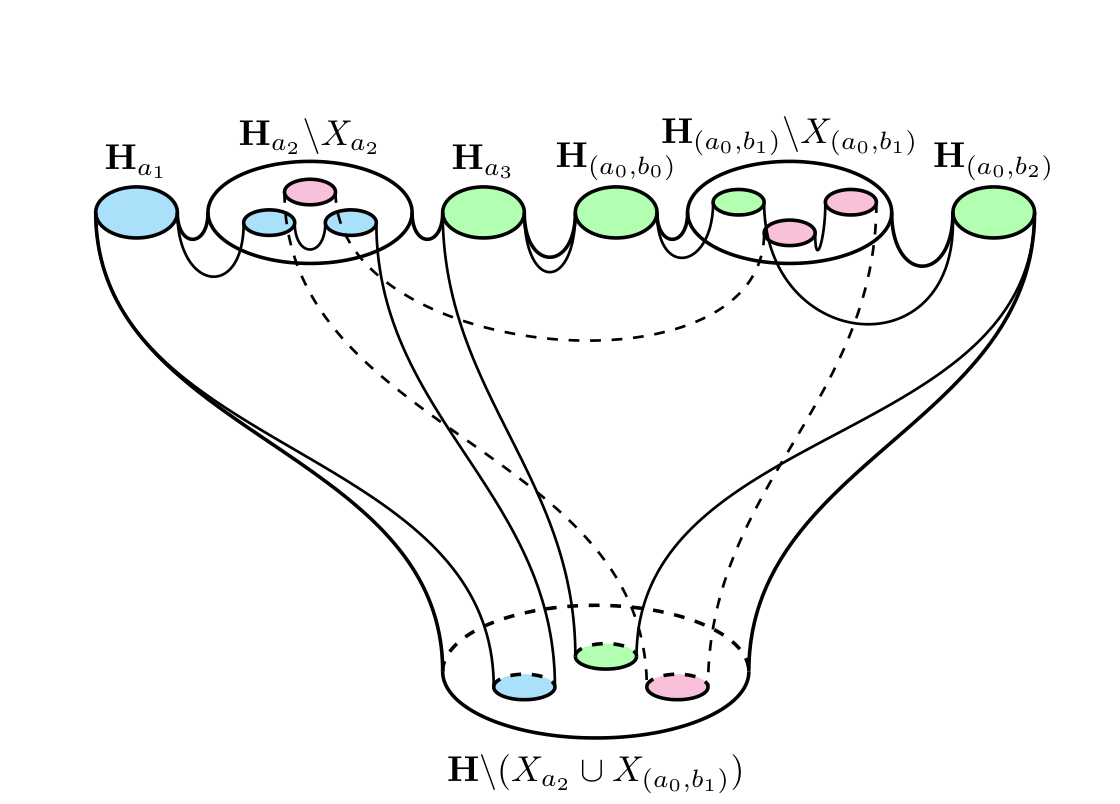
\includegraphics[width=280pt]{../assets/611/cobord-first.png} 
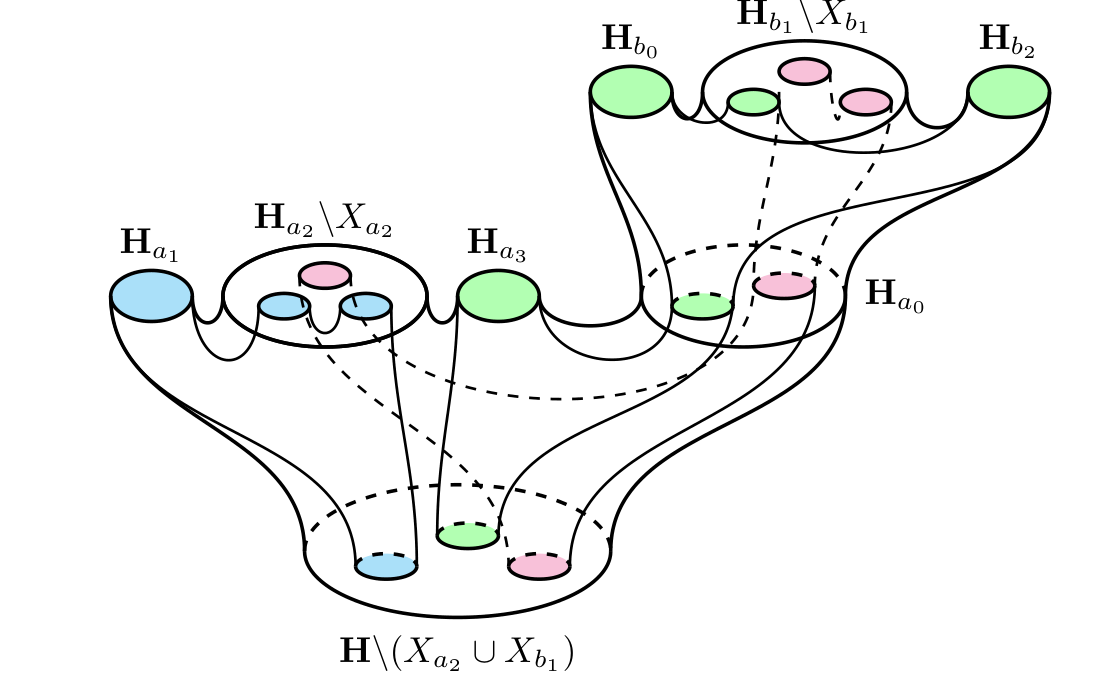
\includegraphics[width=280pt]{../assets/611/cobord-second.png}
%}
\end{center}
\caption{Illustration of associativity via cobordisms, with
$A=\{a_0, \ldots, a_3\}$, 
$A'=\{b_0, \ldots, b_2\}$,
$A''=\{a_1, \ldots, a_3,$ $(a_0, b_0),$ $(a_0, b_1), (a_0, b_2)\}$,
$B'' = \{a_2,(a_0,b_1)\}$, 
$B' = {b_1}$
and $ B = {a_2,a_0}$.
 \label{fig:assoc-cobord}}
\end{figure}

\smallskip\noindent
(1) If $B''\inc A\backslash\set{a_0}$, then, setting ${\bf C}_{a_0}:=\ast^{\tau'}(\delta')$,   we have (using Lemma \ref{linear-construct-in-product}):
$$\ast^{\tau}_{B''}(\delta)= X_{B''}(\ast(\delta^{B''}_1),\dots,\ast(\delta^{B''}_{n_{B''}})),$$
where, for $1\leq l\leq n_{B''}$,
$$\delta^{B''}_l=(\{C_{\tilde{a}}:{\bf H}_{\tilde{a}}\,|\, \tilde{a}\in\tilde{A} \mbox{ and } \varphi_{\tau}^{B''}(\tilde{a})=l\},{\bf H}^{B''}_l),$$
with the indexing set
$$\tilde{A}:=A\backslash
 B''\cup\{(b,p)\,|\, b\in B'' \mbox{ and } 1\leq p\leq n_b\}$$ arising
 from  ${\bf H}_b, X_b\leadsto \hyper{H}_{(b,1)},\dots, \hyper{H}_{(b,n_b)}$ ($b\in B''$).  
Then, establishing  $\ast_{B''}^{\tau''}(\delta'')=\ast_{B''}^{\tau}(\delta)$ amounts to showing  that 
$\ast((\delta'')^{B''}_l)=\ast(\delta^{B''}_l)$, for all $1\leq l\leq n_{B''}$. 

Let $\pi'':\widetilde{A''}\rightarrow A''$ and $\pi:\tilde{A}\rightarrow A$ be the obvious projections (cf. proof of Lemma \ref{Jovana-lemma}). Then it is readily seen (remembering that $H_{(a_0,a')}\inc H_{a_0}$) that $(\pi'')^{-1}(A\backslash\set{a_0})= \widetilde{A''} \cap \tilde{A}= \pi^{-1}(A\backslash\set{a_0})$ and
\begin{equation}
\label{phi-phi-case1}
\varphi_\tau^{B''}|_{\widetilde{A''} \cap \tilde{A}}=\varphi_{\tau''}^{B''}|_{\widetilde{A''} \cap \tilde{A}}\quad \mbox{ and }\quad
\varphi_{\tau}^{B''}\!(a_0)=\varphi_{\tau''}^{B''}(a_0,a'), 
\end{equation}
for all $a'\in A'$. It follows that  for $l\neq \varphi_{\tau}^{B''}(a_0):=l_0$ we have that $(\delta'')^{B''}_l=\delta^{B''}_l$, while (remembering the definition of ${\bf C}_{a_0}$) the equality
$\ast((\delta'')^{B''}_{l_0})=\ast(\delta^{B''}_{l_0})$ follows by induction on $\hyper{H}_{a_0}$.

\medskip\noindent
(2) For $B''\not\inc A\backslash\set{a_0}$, let  ${B}:=(B''\inter(A\backslash\set{a_0}))\union \set{a_0}$ and ${B'}:=\setc{a'\in A'}{(a_0,a')\in B''}$.   Let $X_{{B'}}:=\bigcup_{b'\in {B'}} X_{(a_0,b')}$ and suppose that  ${\bf H}_{a_0}, X_{{B'}}\leadsto (\hyper{H}_{a_0})_1^{{B'}},\dots,(\hyper{H}_{a_0})^{{B'}}_{m_{{B'}}}$.  We have by definition
$$\ast_{B'}^{\tau'}(\delta')=X_{{B'}}(\ast((\delta')^{{B'}}_1),\dots,\ast((\delta')^{{B'}}_{m_{{B'}}})),$$
where, for $1\leq j\leq m_{{B'}}$, 
$$(\delta')^{{B'}}_{j}=(\{C_{\widetilde{a'}}:{\bf H}_{\widetilde{a'}}\,|\, \widetilde{a'}\in \widetilde{A'} \mbox{ and } \varphi_{\tau'}^{{B'}}(\widetilde{a'})=j\},({\bf H}_{a_0})^{{B'}}_{j}),$$
with the indexing set 
%\begin{align*}
$$\quad\quad\widetilde{A'}:=\{(a_0,a')\,|  \,a'\in A'\backslash B'\}\} 
\cup \{(a_0,b',k)\,|\, b'\in B' \text{ and } 1\leq k\leq n_{b'}\}$$
%\end{align*}
arising from  $H_{(a_0,b')}, X_{(a_0,b')}\leadsto \hyper{H}_{(a_0,b',1)},\dots,\hyper{H}_{(a_0,b',n_{b'})}$ ($b'\in B'$). Setting  ${\bf C}^{B'}_{a_0}:=X_{B'}(\ast((\delta')^{B'}_1),\dots,\ast((\delta')^{B'}_{m_{B'}}))$, the equality that we aim to prove displays as  
\begin{equation}
\label{eqcont}
\ast_{B''}^{\tau''}(\delta'')=\ast_{B}^{\tau}(\{C_a\,|\, a\in A\backslash\{a_0\}\}\cup\{{\bf C}^{B'}_{a_0}\}).
\end{equation}
Furthermore, by setting $X_{a_0}:=X_{{B'}}$ and $X_{{B}}:= \bigcup_{b\in {B}}X_b$, we can write 
$$X_{B''}=(\bigcup_{b\in {B}\backslash\{a_0\}}X_b)\bigcup \set{X_{{B'}}}= (\bigcup_{b\in {B}\backslash\{a_0\}}X_b)\bigcup \set{X_{a_0}} =
X_{{B}}.$$
We can then  transform \eqref{eqcont}  (applying Lemma \ref{rooted-linear-construct-in-product})
into 
\begin{equation}
X_{B}(\ast((\delta'')^{B''}_1),\dots,\ast((\delta'')^{B''}_{n_{B''}}))=  
X_{{B}}(\ast(\delta^{{B}}_1),\dots,\ast(\delta^{{B}}_{n_{{B}}})),
\end{equation}
where
${\bf H}, X_{{B}}\leadsto \hyper{H}_1^{{B}},\dots,\hyper{H}^{{B}}_{n_{{B}}}$, $n_{{B}}=n_{B''}$, and
for $1\leq l\leq n_{{B}}$, 
$$\delta^B_l=(\{C_{\tilde{a}}:{\bf H}_{\tilde{a}}\,|\, \tilde{a}\in\tilde{A} \mbox{ and } \varphi_{\tau}^{{B}}(\tilde{a})=l\},{\bf H}^{{B}}_l),$$
with the indexing set 
$$\tilde{A}:=A\backslash {B}\cup\{(b,p)\,|\, b\in {B} \mbox{ and } 1\leq p\leq n_b\}$$
arising from ${\bf H}_b, X_b\leadsto \hyper{H}_{(b,1)},\dots,\hyper{H}_{(b,n_b)}$ ($b\in {B}$),
and where 
$$C_{\tilde{a}}=\begin{cases}
C_a, & \mbox{ if } \tilde{a}\in (A\backslash {B}),\\
%C^{\underline{B'}}_{a_0}, & \mbox{ if }\tilde{a}=a_0\in A\backslash {B},\\
\ast((\delta')^{{B'}}_{p}), & \mbox{ if } \tilde{a}=(a_0,p),\\
C_{(b,p)}, & \mbox{ if } \tilde{a}=(b,p) \quad(b\in {B}\backslash\set{a_0}).
\end{cases}$$
 Now, since $X_{B''}=X_{\plunderline{B}}$, 
we can suppose, without loss of generality, that $H_{i}^{B''}=H^{\plunderline{B}}_{i}$, for all $1\leq i\leq n_{\plunderline{B}}=n_{B''}$. Therefore, it remains to show that $\ast((\delta'')^{B''}_{i})=\ast(\delta_i^{\plunderline{B}})$. Observe that, since $$\quad\quad\quad \hyper{H}_{(a_0,1)},\dots,\hyper{H}_{(a_0,n_{a_0})}\reflectbox{$\leadsto$}\,{\bf H}_{a_0}, X_{a_0}={\bf H}_{a_0}, X_{\plunderline{B'}}\leadsto (\hyper{H}_{a_0})_1^{\plunderline{B'}},\dots,(\hyper{H}_{a_0})^{\plunderline{B'}}_{m_{\plunderline{B'}}},$$
we have that $n_{a_0}=m_{\plunderline{B'}}$, and  we can assume (without loss of generality) that $H_{(a_0,p)}=(H_{a_0})^{\plunderline{B'}}_p$, for each $1\leq p\leq n_{a_0}$.   

Simple inspection (and standard argumentation with connected components) yields
$$\begin{array}{l}
\pi''^{-1}(A\backslash\set{a_0})= \widetilde{A''}\cap \tilde{A} = \pi^{-1}(A\backslash\set{a_0})\\
\pi''^{-1}(a_0) = \widetilde{A'},
\end{array}$$
where $\pi'':\widetilde{A''}\rightarrow A''$  and $\pi:\tilde{A}\rightarrow A$  are the obvious projections,
and  
\begin{equation} \label{phi-phi-case2}
\varphi^{B''}_{\tau''}|_{\widetilde{A''}\cap \tilde{A}}=\varphi_{\tau}^{\plunderline{B}}|_{\widetilde{A''}\cap \tilde{A}} \quad\mbox{ and }\quad  \varphi^{B''}_{\tau''}|_{\widetilde{A'}}=\tilde{\varphi}^{\plunderline{B}}_{\tau}\circ\varphi^{\plunderline{B'}}_{\tau'},\end{equation} 
where  
$\tilde{\varphi}_{\tau}^{\plunderline{B}}(j):={\varphi}_{\tau}^{\plunderline{B}}((a_0,j))$, for each $1\leq j\leq n_{a_{0}}$.
We  note that, thanks  to \eqref{phi-phi-case2}, $\ast((\delta'')^{B''}_{i})$ and $\ast(\delta_i^{\plunderline{B}})$ look respectively like this:
 $$\begin{array}{lll}
\quad \quad\quad \ast((\delta'')^{B''}_{i}) & = &  \ast(\underbrace{\ldots, C_y, \ldots}_{y\in \tilde{A}''\cap \tilde{A},\varphi_{\tau''}^{B''}(y)=i}\,\,\,\,\,\,,\:\ldots\:,\,\underbrace{\ldots ,C_x, \ldots}_{x\in \tilde{A}',\, \varphi^{\plunderline{B'}}_{\tau'}(x)=j\in (\tilde{\varphi}_{\tau}^{\plunderline{B}})^{-1}(i)}  \,\,\,\;,\ldots)\\
\quad\quad\quad\ast(\delta_i^{\plunderline{B}}) &=& \ast(\underbrace{\ldots, C_{y},\ldots}_{y\in \widetilde{A''}\cap \tilde{A},\varphi_{\tau}^{\plunderline{B}}(y)=i}\,\,\,\,\,\,,\:\ldots\:,\,\underbrace{\ast(\ldots, C_x, \ldots)}_{x\in \tilde{A}',\, \varphi^{\plunderline{B'}}_{\tau'}(x)=j\in (\tilde{\varphi}_{\tau}^{\plunderline{B}})^{-1}(i)}  \,\,\,\;,\ldots)
 \end{array}$$  
 and we conclude by applying   induction  to each $\hyper{H}^{B''}_i$ (note that repeated induction, or no induction at all, may be needed for a single fixed $i$, depending on the cardinality of 
 $\varphi^{\plunderline{B'}}_{\tau'}(\tilde{A})
 \cap (\tilde{\varphi}_{\tau}^{\plunderline{B}})^{-1}(i)$).

This concludes the proof of the polydendriform equation.
Associativity is derived as follows. Writing $\delta_{B'}$ for $\{C_a\,|\,a\in A\backslash\{a_0\}\}\cup \{\ast^{\tau'}_{B'}(\delta')\}$, we have  on one hand (in-lining the polydendriform equation):
$$\begin{array}{lllll}
\ast^{\tau''}(\delta'') & = & \overbrace{\sum_{\emptyset\incs B''\subseteq A\backslash\set{a_0}} q^{{|B''|}-1} \:\ast^{\tau}_{B''}(\delta)}^{A_1} & +
& \overbrace{\sum_{\emptyset\incs B''\not\subseteq A\backslash\set{a_0}} q^{{|B''|}-1} \:\ast^{\tau}_B(\delta_{B'})}^{B_1}\\
\end{array}
$$
with $B,B'$ determined from $B''$ as specified in the statement, and on the other hand  (expanding the second summand by linearity):
$$
\ast^{\tau}(\delta)\; =\;  \underbrace{\sum_{\emptyset\incs B\subseteq A\backslash\set{a_0}} q^{{|B|}-1} \:\ast^{\tau}_{B}(\delta)}_{A_2} \; + \;
\underbrace{\sum_{\emptyset\incs B\not\subseteq A\backslash\set{a_0}}  \sum_{\emptyset\incs B'\subseteq A'}q^{|B|+|B'|-2} \:\ast^{\tau}_B(\delta_{B'})}_{B_2}
$$
We have $A_1=A_2$ literally, while $B_1=B_2$ follows by noticing that the map $B''\mapsto ((B''\cap(A\backslash\{a_0\}))\cup\{a_0\},\{a'\in A'\,|\, (a_0,a')\in B''\})$ is bijective. 
\end{proof}

 



\begin{remark} One could formulate the polydendriform structure as an algebra over a colored operad, where the colors are hypergraphs, the operations are teams, and the carrier of the algebra for the color $\hyper{H}$ is the set of constructs of $\hyper{H}$.
\end{remark}

We shall now relate the polydendriform structure to the tridendriform one, by showing that  the former implies (and can be considered as the unbiased version of) the latter, in the {\em ordered}   framework. 

Let $\Xi$ be an ordered associative clan. Suppose that we have 
$$\{((\hyper{H}_1,\hyper{H}_{2'}),\hyper{H}),   ((\hyper{H}_2,\hyper{H}_{3}),\hyper{H}_{2'}), 
((\hyper{H}_{1'},\hyper{H}_{3}),\hyper{H}),  ((\hyper{H}_1,\hyper{H}_{2}),\hyper{H}_{1'})\}\in\Xi.$$ Denote by $\tau''_1$ the grafting of $((\hyper{H}_1,\hyper{H}_{2}),\hyper{H}_{1'})$ to $((\hyper{H}_{1'},\hyper{H}_{3}),\hyper{H})$ along $1'$, and by $\tau''_2$ the grafting of $((\hyper{H}_2,\hyper{H}_{3}),\hyper{H}_{2'})$ to $((\hyper{H}_1,\hyper{H}_{2'}),\hyper{H})$ along $2'$.  
Note that the above teams are all of the (generic) form
$((\hyper{H}_l,\hyper{H}_r),\hyper{L})$.
We write (cf. Example \ref{permutohedra- })
$$\prec\,:=\ast_{\set{l}} \quad\quad \bcdot\,:=\ast_{\set{l,r}} \quad\quad \succ\,:=\ast_{\set{r}}.$$ 
\begin{proposition} \label{poly-implies-tri}
In the ordered framework, the tridendriform equations follow from the polydendriform one, relatively to the team $\tau''=((\hyper{H}_1, \hyper{H}_2, \hyper{H}_3), \hyper{H})$.
More precisely, Loday--Ronco's seven equations, as listed in the introduction, correspond to  choosing $B''$ to be $\set{1}$, $\set{2}$, $\set{3}$, $\set{1,2,3}$, $\set{2,3}$, $\set{1,3}$, $\set{1,2}$, respectively.
\end{proposition}
\begin{proof} 
As a sanity check, we first note that there are $2^3-1=7$ non-empty subsets of $\set{1,2,3}$. We check the equation $(\succbcdot)$. Let
$S:\hyper{H}_1$, $T:\hyper{H}_2$, $U:\hyper{H}_3$. We have
{\small
$$
\ast^{\tau''_1}_{\set{2,3}} (S,T,U)  =  \ast_{\set{1',3}}((\ast_{\set{2}}(S,T),U))=   ((S \succ T) \bcdot U)$$
and $$ \ast^{\tau''_1}_{\set{2,3}} (S,T,U)  = \ast^{\tau''_2}_{\set{2,3}} (S,T,U) =  \ast_{\set{2'}} (S,(\ast_{\set{2,3}}(T,U))) = S \prec (T \bcdot U).$$}
Note that all tridendriform equations follow from the second case of the polydendriform equation, except  $(\precstar)$  and  $(\astsucc)$ (for which we use the first case, and which are the only tridendriform equations involving $\ast$).
\end{proof}


Combining the results of \S\ref{restrictohedra-section} and \S\ref{asp}, we get a whole range of polydendriform/tridendriform structures, and in particular we get structures associated with the graphs  $\mathbf{\Gamma}^k$ of Proposition \ref{Gamma-order-friendly}. As we have seen,
for the instances $k=1$ and $k=\infty$, we recover the tridendriform structures of \S\ref{Prologue-section}, thus fulfilling our unifying goal, with a whole infinity of examples sitting ``in the middle''. The case k=2 is that of friezohedra.

\begin{remark} The associative product defined here is quite different (both in form and spirit) from the algebraic structure on the constructs of all graph associahedra  defined by Forcey and Ronco in \cite{FR}, which provides an example of reconnectad, as defined and investigated in \cite{DotsenkoReconnectad}.  We first note that the definitions of \cite{FR, DotsenkoReconnectad} can be straightforwardly upgraded to nestohedra.  For a contrast, we briefly introduce the Forcey-Ronco products, using notation akin to the ones used here. Our teams are replaced by the data of 
a (hyper)graph $\hyper{H}$ and a non empty subset $X\inc H$, giving rise to a ``reconnecteam'' 
$((\hyper{H}_{\cap X},\hyper{H}_1,\ldots,\hyper{H_n}),\hyper{H})$, where $\hyper{H}_{\cap X}$ is the so-called reconnected restriction of $\hyper{H}$ to $X$ whose hyperedges are the intersections of the tubes  of $\hyper{H}$ with $X$, and where $\hyper{H},X\leadsto \hyper{H}_1,\ldots, \hyper{H}_n$. Now, given constructs $S:\hyper{H}_{\cap X}$, $T_1:\hyper{H}_1$, \ldots, $T_n:\hyper{H}_n$, the operad-like composition $(\circ_X^{\hyper{H}}(S;T_1,\ldots,T_n)):\hyper{H}$  is obtained by substituting $S$ for $X$, $T_1$ for $H_1$, \ldots, $T_n$ for $H_n$ in the codimension 1 construct
$(X(H_1,\ldots,H_n)):\hyper{H}$. 
The underlying combinatorics in \cite{FR} is thus substitution in nodes of trees, while in our work it is that of  shuffles of trees. Another key difference is that in our teams the participant hypergraphs are not determined by the coordinating hypergraph. 
As a final remark, the underlying ``universe" of Forcey-Ronco is the collection of all (hyper)graphs, in contrast to the situation here.
\end{remark}


\subsection{A non-recursive definition of the product} \label{non-recursive}

In this subsection, we give an equivalent, non-recursive, definition of the product, directly inspired from \cite{RoncoGTO}. 
 Let $\hyper{H},\hyper{L}$ be two connected hypergraphs such that $H\inc L$ and such that, for all $e\in\hyper{H}$, $e$ is a tube of  $\hyper{L}$. This entails in particular that $H$ is a tube of  $\hyper{L}$. Let $S=X(S_1,\ldots,S_n)$  be a construct of $\hyper{L}$, with $S_i:\hyper{L}_i$ where $\hyper{L},X\leadsto\hyper{L}_1,\ldots,\hyper{L}_n$. Then we define a construct $\restrconstr{S}{\hyper{H}}:\hyper{H}$, called the {\em restriction of $S$ to} $\hyper{H}$, as follows. We distinguish two cases.
\begin{itemize}
\item
If $X\cap H=\emptyset$, then there is a unique $j$ such that
$H\inc L_j$, and we set $$\restrconstr{S}{\hyper{H}}=\restrconstr{(S_j)}{\hyper{H}}.$$
\item
If $X\cap H\neq\emptyset$, let $\hyper{H},(X\cap H)\leadsto \hyper{H}_1,\ldots,\hyper{H}_p$. This determines a function $\varphi_X^{\hyper{H},\hyper{L}}:\set{1,\ldots,p}\rightarrow\set{1,\ldots,n}$, and we set  $$\restrconstr{S}{\hyper{H}}=(X\cap H)(\ldots,\restrconstr{(S_{\varphi_X^{\hyper{H},\hyper{L}}(i)})}{\hyper{H}_i},\ldots).$$
\end{itemize}
That  $\restrconstr{S}{\hyper{H}}$ is indeed a construct of $\hyper{H}$ is easily seen by induction.   

\begin{example} \label{4.19} In the universe of friezohedra, let us consider $\hyper{H}=\hyper{F}_{\{1, 3, 5\}}$ and $\hyper{L}=\hyper{F}_{\{1, \ldots, 5\}}$. As every edge in $\hyper{H}$ is also in $\hyper{L}$, the hypothesis above is satisfied. Consider the construct $S=3(\{1,4\}(2,5))$ of $\hyper{L}$. Then $\restrconstr{S}{\hyper{H}}=3(1,5)$. \demo
\end{example}

We next give a simpler (but more ``mysterious'')  alternative description of  $\restrconstr{S}{\hyper{H}}$ in terms of nested sets (see Remark \ref{tub}). In order to formulate the lemma, we need one definition (generalized from \cite{RoncoGTO} to the setting of hypergraph polytopes). With each tube $t$  of $\hyper{L}$ we associate a construct $t_{\hyper{H}}$ as follows (note the heterogeneous nature of this definition: we go from tubes to constructs):
\begin{itemize}
\item If $H\inc t$, then we set $t_{\hyper{H}}=H$;
\item if $H\backslash t\neq\emptyset$ yielding $\hyper{H},(H\backslash t)\leadsto \hyper{H}_1,\ldots,\hyper{H}_k$, we set $t_{\hyper{H}}=(H\backslash t)(H_1,\ldots,H_k)$. 
\end{itemize}
This definition can be seen as an instantiation of our definition of $\restrconstr{S}{\hyper{H}}$: more precisely, we can coerce a tube $t$ of $\hyper{L}$ to a construct  $(L\backslash t)(t):\hyper{L}$, and we have 
$t_{\hyper{H}} = \restrconstr{((L\backslash t)(t))}{\hyper{H}}$.

The following proposition 
gives a non-recursive definition for the above restriction operation,
providing a bridge between our  definition and that of Ronco in \cite{RoncoGTO}.


\begin{proposition} \label{restrconst-as-tubing}
For $\hyper{H},\hyper{L}$ and $S$ as above, we have $\psi(\restrconstr{S}{\hyper{H}})=
\bigcup\setc{\psi(t_{\hyper{H}})}{t\in\psi(S)}$.
\end{proposition}
\begin{figure}
\begin{center}
%\resizebox{\textwidth}{!}{
%\includegraphics[scale=0.3]{Figure-pour-lemme-4.pdf}
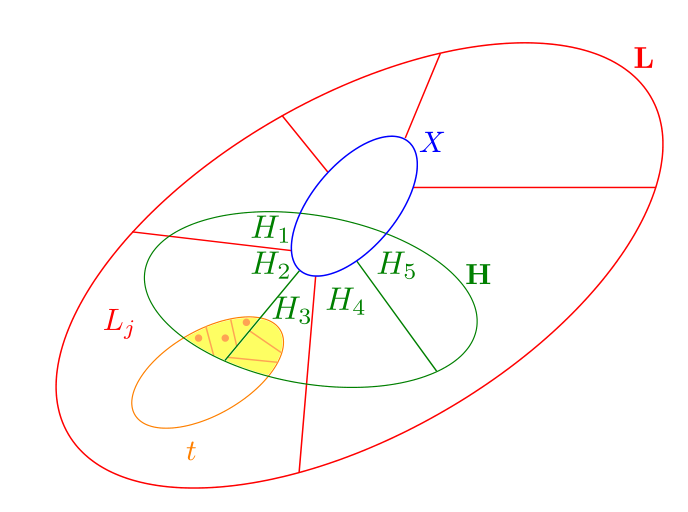
\includegraphics[width=172pt]{../assets/611/restriction-graphic.png} 
%}
\end{center}
{\small \begin{itemize}
\item The compartments with red/blue border are the connected components of $\hyper{L}\backslash X$. 
\item The compartments with green/red/blue border are the connected components of $\hyper{H}\backslash X$.
\item In this example, we have $(\varphi_X^{\hyper{H},\hyper{L}})^{-1}(j)=\set{2,3}$.
\item The small yellow compartments with orange/green borders feature the tubes in $\psi(t_{\hyper{H}})$, 
\item while those additionally marked with a dot are the tubes in $\psi(t_{\hyper{H}_2})$.
\end{itemize}}
\caption{Illustration of the proof of Lemma  \ref{restrconst-as-tubing} \label{restrconst-as-tubing-illust}}
\end{figure}
\begin{proof} (Sketch) Let $S=X(S_1,\ldots,S_n)$ and $L\neq t\in\psi(S)$, i.e. $t\in\psi(S_j)$ for some $j$. Then the statement follows from the  observation (illustrated in Figure \ref{restrconst-as-tubing-illust}) that, with the notation introduced above:
$$\psi(t_{\hyper{H}})= \bigcup\setc{\psi(t_{\hyper{H}_i})}{\varphi_X^{\hyper{H},\hyper{L}}(i)=j} \quad (j,t\in\psi(S_j)\;\mbox{fixed}, i\;\mbox{varying}).$$
Indeed, by definition of $\psi$, we have on one hand that  $(\bigcup\setc{\psi(t_{\hyper{H}})}{t\in\psi(S)})\backslash\set{H}$ is the union of the sets
$(\bigcup\setc{\psi(t_{\hyper{H}})}{t\in\psi(S_j)})$, indexed by $1\leq j\leq n$. On the other hand, applying induction, we have that $\psi(\restrconstr{S}{\hyper{H}})\backslash\set{H}$ is the union of the sets $\psi(t_{\hyper{H}_i})$, for $1\leq i\leq p$ and $t\in \psi(S_{\varphi_X^{\hyper{H},\hyper{L}}(i)})$, which we can repackage as a union indexed by  $j$ (gathering all $i$ such that $\varphi_X^{\hyper{H},\hyper{L}}(i)= j$).  We then conclude by the observation.\end{proof}
In particular, via the characterization of tubings as constructs, Proposition \ref{restrconst-as-tubing} says that the definition in terms of tubings given in    \cite{RoncoGTO} returns indeed a tubing.

We now come back to the promised alternative definition of the   product. 
Let $\tau=(\{{\bf H}_a\,|\,a\in A\},{\bf H})$ be a team and $U=X(U_1,\ldots,U_n)$ be a construct of $\hyper{H}$. We  associate with $U$ a ``measure''  $\mu^\tau(U)$ as follows (with the notation of \S\ref{tcd}).  We set $B=\setc{b\in A}{X\cap H_b\neq\emptyset}$ and $X_b=X\cap H_b$ for each $b\in B$ (so that $n=n_B$), and we set
$$\mu^\tau(U)=(|B|-1)+ \sum_{1\leq i\leq n_B}\mu^{\tau_i}(U_i).$$The following proposition gives a non-inductive characterization of our product $\ast$.
\begin{proposition} \label{restriction-product-characterization} Let $\Xi$ be a strict clan, and
let $\delta=(\{C_a:{\bf H}_a\,|\, a\in A\},{\bf H})$ be a $\Xi$-delegation of support $\tau$. Then we have:
$$\ast(\delta)= \sum_{U:\hyper{H} \;\mbox{{\small and}}\; \forall a\in A, \restrconstr{U}{\hyper{H}_a}=C_a} q^{\mu^\tau(U)}\, U,$$
and for each $\emptyset\neq B\inc A$, we have that $q^{|B|-1} (\ast_B(\delta))$ is the summand of the above sum where $U$  is further constrained to be such that $\mbox{root}(U)=X_B$.
\end{proposition}
\begin{proof} (Sketch) We use the same notations as above. By unfolding the definition of $U=X(U_1,\ldots,U_n)$, with $X=X_B$, the constraints on $U$ boil down to the constraints (for each $i$) $\restrconstr{(U_i)}{\hyper{H}_{\tilde{a}}}=C_{\tilde{a}}$  for all $\tilde{a}\in\tilde{A}$ such that
$\varphi^{\tau}_B(\tilde{a})=i$. This entails that, taking the right-hand side of the equality and its summands   in the statement as a definition of $\ast$ and $\ast_B$, and noticing that
\begin{equation*}
q^{\mu^\tau(U)}\, X_B(U_1,\ldots,U_n)= q^{|B|-1}\, X_B(\ldots,q^{\mu^{\tau_i}(U_i)}\, U_i,\ldots),
\end{equation*}
 these definitions satisfy the equation $\ast_B(\delta)=(\Union_{b\in B}X_b)(\ast(\delta^B_1),\dots,\ast(\delta^B_{n_{B}})$.
\end{proof}

\begin{remark}\label{Ronco-specialize} 
In the ordered setting, and in the special case  where $q=1$  and where teams have the form $((\hyper{H}_{H_1},\hyper{H}_{H_2}),\hyper{H})$), the summation in the statement of Proposition \ref{restriction-product-characterization}
 is  the definition of associative product given in  \cite[Theorem 3.19]{RoncoGTO}. This justifies our  earlier claim that our product specializes to Ronco's setting.
\end{remark}
\begin{example}
We consider the delegation of friezohedra $$\delta=(\{3(1,5)\!:\!\hyper{F}_{\{1,3,5\}}\,,\, 4(2)\!:\!\hyper{F}_{\{2,4\}}\},\hyper{F}_{\{1,2,3,4,5\}}).$$ The   shuffle product of $\delta$ is then given, up to some coefficients, by the sum of all the constructs $U$ of $\hyper{F}_{\{1,\ldots,5\}}$ such that  
$\restrconstr{U}{\hyper{F}_{\{1,3,5\}}} = 3(1,5)$ and $\restrconstr{U}{\hyper{F}_{\{2,4\}}} = 4(2)$. The power of $q$ in the coefficient of $S=3(\{1,4\}(2,5))$ in this sum is given by:
\begin{align*}
\mu^{(\{\hyper{F}_{\{1,3,5\}}, \hyper{F}_{\{2,4\}}\},\hyper{F}_{\{1,2,3,4,5\}})}(S)&= (1-1)+ \mu^{(\{\hyper{F}_{\{1\}}, \hyper{F}_{\{5\}}, \hyper{F}_{\{2,4\}}\},\hyper{F}_{\{1,2,4,5\}})}(\{1,4\}(5(2)) \\
   &= (2-1)+ \mu^{(\{\hyper{F}_{\{2\}}\},\hyper{F}_{\{2\}})}(2) +\mu^{(\{\hyper{F}_{\{5\}}\},\hyper{F}_{\{5\}})}(5)  \\
  &= 1+ (1-1) + (1-1)=1.  \demo
\end{align*} 

\end{example}

We note that the non-recursive definition leads to another proof of the polydendriform equation and of associativity -- that is technically  simpler but geometrically less appealing than the one we gave in \S\ref{asp}, based on the observation, say for $(\{{\bf H}_1,{\bf H}_2,{\bf H}_3\},{\bf H})$, $(\{{\bf H}_1,{\bf H}_2\},{\bf H}_{12})$,  $(\{{\bf H}_{12},{\bf H}_3\},{\bf H})$, and $$\delta=(\{S\!:\!{\bf H}_1\,,\, T\!:\!{\bf H}_2\,,\,U\!:\!{\bf H}_3\}\,,\,{\bf H}),$$
 that the data of $V:\hyper{H}$ such that $\restrconstr{V}{\hyper{H}_1}=S$, $\restrconstr{V}{\hyper{H}_2}=T$ and 
 $\restrconstr{V}{\hyper{H}_3}=U$ is equivalent to the data of $V:\hyper{H}$ and $W:\hyper{H}_{12}$ such that $\restrconstr{W}{\hyper{H}_1}=S$, $\restrconstr{W}{\hyper{H}_2}=T$, $\restrconstr{V}{\hyper{H}_{12}}=W$, and $\restrconstr{V}{\hyper{H}_3}=U$ \footnote{In turn, this observation relies on the composability of restrictions, i.e. one can prove that 
$(\restrconstr{V}{\hyper{H}_{12}})\restrconstr{{}}{\hyper{H_1}}= \restrconstr{V}{\hyper{H}_1}$.}.
 

\subsection{Extending the framework}\label{quasi-strict-subsection} 

In this subsection, we enlarge the coverage of our formalism of teams and clans, and we adapt the   product accordingly, in order to cover other families of polytopes like simplices, hypercubes, or erosohedra. 

A preteam $\tau=(\{{\bf H}_a\,|\,a\in A\},{\bf H})$ is called a {\it quasi-strict team} if  for each choice of a   subset $\emptyset\neq B\inc A$ and of a subset $\emptyset\neq X_b\subseteq H_b$ for each $b\in B$, we have that, for each $\tilde{a}\in \tilde{A}$,  

\begin{enumerate}
\item[(1)] $H_{\tilde{a}}$ is included  in a connected component of $\restrH{H}{(\Union_{b\in B}X_b)}$, or
\item[(2)] $|H_{\tilde{a}}|\geq 2$, and, for all  $x\in H_{\tilde{a}}$, $\set{x}$ is a connected component of  $\restrH{H}{(\Union_{b\in B}X_b)}$,
\end{enumerate}
where $\tilde{A}$ is as in \S\ref{tcd}.  When (2) applies (and vacuously when $|H_{\tilde{a}}|=1$), we say that $\hyper{H}_{\tilde{a}}$ is {\em dissolved} in $\restrH{H}{(\Union_{b\in B}X_b)}$.
Let us denote with $\tilde{A}_d$ the set of elements $\tilde{a}$ of $\tilde{A}$ such that  case (2) applies.
We  define 
$\overline{A}$ by removing from $\tilde{A}$ all elements $\tilde{a}$ of $\tilde{A}_d$ and replacing them by the elements of $H_{\tilde{a}}$ (thus expressing the atomization of $\hyper{H}_{\tilde{a}}$), for all $\tilde{a}\in \tilde{A}_{d'}$, i.e. 
$\overline{A}:=(\tilde{A}\backslash \tilde{A}_d) + \union_{\tilde{a}\in \tilde{A}_d} H_{\tilde{a}}$.
The whole situation determines a partition $\overline{A}=\overline{A}_1\union\ldots\union \overline{A}_{n_B}$, and $n_B$ preteams $\tau_i =(\setc{\hyper{H}_{\overline{a}}}{\overline{a}\in \overline{A}_i},\hyper{H}_i)$, where $\hyper{H}_{\overline{a}}$ is defined on the new elements 
$\overline{x}\in  \union_{\tilde{a}\in \tilde{A}_d} H_{\tilde{a}}$
as $\hyper{H}_{\overline{x}}=\set{\set{\overline{x}}}$.
We still use the notation 
$\displaystyle{\tau,\Union_{b\in B}X_b\clandec \tau_1,\ldots,\tau_{n_B}.}$

The definition of clan is unchanged, except that a clan now consists of quasi-strict teams and not of strict teams.
The definition of the    product  is adapted as follows. We assign a  construct $C_{\overline{a}}$ of $\hyper{H}_{\overline{a}}$ for all $\overline{a}\in \overline{A}$, via the following adjustment with respect to the strict case: if $\overline{x}$ is an element of $H_{\tilde{a}}$ for some $\tilde{a}\in \tilde{A}_d$, then we set $C_{\overline{x}}=\set{\overline{x}}$, and we finish as in the strict case: the assignment determines delegations
$\delta_i^B$  $(1\leq i\leq n_B)$, and we define the product exactly as in (\ref{shuffle-def}), but setting $q=-1$ (see below).

We can still define a function $\varphi_{\tau}^B$ from $\tilde{A}\backslash\tilde{A}_d$ to $\set{1,\ldots,n_B}$, which we prefer to see as a partial function from $\tilde{A}$ to $\set{1,\ldots,n_B}$. Abusing notation, we can still write (cf. (\ref{deltas}))
$\delta^B_i=(\{C_{\tilde{a}}:{\bf H}_{\tilde{a}}\,|\, \tilde{a}\in \tilde{A} \mbox{ and }\varphi_\tau^B(\tilde{a})=i\},{\bf H}_i^B),$
noticing  that the  participating hypergraphs of  $\tau_i$ that are not the hypergraphs  ${\bf H}_{\tilde{a}}$ with 
$\tilde{a}\in (\varphi_\tau^B)^{-1}(i)$
are all singleton graphs, so that the sloppy notation above extends in a unique way to the ``true'' definition of $\delta^B_i$.

Note however that our abuse of notation is not as innocent as it seems, since the convention relies on the fact that a singleton hypergraph 
$\set{\set{a}}$ admits a unique {\it plain} construct $a$. 
But the same hypergraph admits all $\lambda a$ ($\lambda\in\Bbbk$) as {\it linear} constructs -- a fact that is stressed in the following remark.



\begin{remark} \label{dissolution-irrelevance}
It follows from the definitions that
if $\delta_1$ and $\delta_2$ are delegations of plain constructs having the same support $\tau=(\setc{\hyper{H}_a}{a\in A},\hyper{H})$, if $\delta_1$ and $\delta_2$ differ only on one participating hypergraph $\hyper{H}_{a_0}$,  if $B$ is a non-empty subset of $A$ such that $a_0\nin B$ and $\varphi_\tau^B(a_0)$ is undefined, then $\ast(\delta_1)=\ast(\delta_2)$.  Moreover, if $\delta$ is a (linear) delegation which coincides with $\delta_1$ and $\delta_2$ on all $a\in A\backslash\set{a_0}$ and has in position $a_0$ a linear construct $\sum_{i\in I} \lambda_i C_i$, then we have $\ast(\delta) = (\sum_{i\in I} \lambda_i) \ast\!(\delta_1) \; (= (\sum_{i\in I} \lambda_i) \ast\!(\delta_2))$.
\end{remark}

The notion of associative clan is unchanged.  
The associativity theorem still holds, but only under the assumption $q\!=\!-1$.  The reason for this restriction stems from Remark \ref{dissolution-irrelevance} and from the following lemma.

\begin{lemma} \label{sum-coeff1} If $q\!\!=\!\!-1$, then, for any delegation (in the quasi-strict setting)  $\delta$ of plain constructs, the sum of all coefficients in the expansion of  $\ast(\delta)$ as a linear combination of plain constructs is equal to $1$.
\end{lemma}
\begin{proof} We prove the statement by induction on $|H|$.
From the binomial expansion
 $(1+x)^n=\sum_{0\leq i\leq n}\binom{n}{i} x^i$ expressed as   $(1+x)^n=1 + x(\sum_{1\leq i\leq n}\binom{n}{i} x^{i-1})$
and instantiated with $x=q= -1$, we readily obtain $\sum_{1\leq i\leq n}\binom{n}{i} q^{i-1}=1$.  The statement will then follow if we prove that, for each $\emptyset\subset B\subseteq A$, the sum of the coefficients in the expansion of  
$X_B(\ast(\delta_1),\ldots, \ast(\delta_{n_B}))$ as a linear combination of plain constructs is equal to $1$. But this in turn follows by induction and by multilinearity.
 \end{proof}

 

\begin{theorem}\label{assoc_quasi_strict}
Theorem \ref{assoc_strict} extends to the quasi-strict setting for $q=-1$.
\end{theorem}
\begin{proof}
Using the convention above of still defining the   product by appealing to the functions $\varphi_\tau^B$,  the proof of Theorem \ref{assoc_strict} goes through, as long as we do not use the totality of these functions. More precisely, the reasoning in case (1) unfolds without change until the equalities (\ref{phi-phi-case1}) included, which still hold but have now to be understood in the partial sense, i.e. the left-hand side is defined if and only if the right-hand side is defined, in which case they are equal. 

Then two subcases arise.
\begin{enumerate}
\item[(1a)] If $\varphi_\tau^{B''}(a_0)$ is defined, then we conclude case (1) by induction as in the proof of Theorem  \ref{assoc_strict}.
\item[(1b)] Suppose   (new case!) that  $\varphi_\tau^{B''}(a_0)$ is undefined.    Let $\ast^{\tau'}(\delta')=\sum_{i\in I}\lambda_i C_i$.  By Lemma \ref{sum-coeff1}, we have 
$\sum_{i\in I}\lambda_i=1$. Let $\delta'_i$ be the delegation obtained by replacing $\ast(\delta')$ by $C_i$ in $\delta$. By Remark \ref{dissolution-irrelevance}, we have 
$\ast_{B''}(\delta'_i)=\ast_{B''}(\delta'_j)$ for all $i,j$, and, calling  $D$  the common value, we have:
$$\ast_{B''}(\delta)= (\sum_{i\in I}\lambda_i) D = D.$$
On the other hand, by (\ref{phi-phi-case1}), we also have that 
$\varphi_{\tau''}^{B''}(a_0,a')$ is undefined (for all $a'\in A'$), and, again, $\ast^{\tau''}(\delta'')$ does not depend on the  constructs $C_{(a_0,a')}$.  
Moreover, observing that $\delta$ and $\delta''$  coincide on the indices $a\in A\backslash\set{a_0}$,  we get easily that
$\ast_{B''}(\delta'')$ is also equal to the common value $D$, which concludes this new case in the proof of associativity.
\end{enumerate}
Similarly, the reasoning in case (2) unfolds without change until the equalities (\ref{phi-phi-case2}) included, which again hold in the partial sense explained above. Let us repeat here the expressions for $ \ast((\delta'')^{B''}_{i})$ and  for $\ast(\delta_i^{\plunderline{B}})$ that we wrote at this point of the proof of Theorem \ref{assoc_strict}:
 $$\begin{array}{lll}
 \ast((\delta'')^{B''}_{i}) & = &  \ast(\underbrace{\ldots, C_y, \ldots}_{y\in \tilde{A}''\cap \tilde{A},\varphi_{\tau''}^{B''}(y)=i}\,\,\,\,\,\,,\:\ldots\:,\,\underbrace{\ldots, C_x, \ldots}_{x\in \tilde{A}',\, \varphi^{\plunderline{B'}}_{\tau'}(x)=j\in (\tilde{\varphi}_{\tau}^{\plunderline{B}})^{-1}(i)}  \,\,\,\;,\ldots)\\
\ast(\delta_i^{\plunderline{B}}) &=& \ast(\underbrace{\ldots ,C_{y},\ldots}_{y\in \widetilde{A''}\cap \tilde{A},\varphi_{\tau}^{\plunderline{B}}(y)=i}\,\,\,\,\,\,,\:\ldots\:,\,\underbrace{\ast(\ldots ,C_x,\ldots)}_{x\in \tilde{A}',\, \varphi^{\plunderline{B'}}_{\tau'}(x)=j\in (\tilde{\varphi}_{\tau}^{\plunderline{B}})^{-1}(i)}  \,\,\,\;,\ldots)
 \end{array}$$
 The   first expression is still correct, as it displays (with $i$ varying) all elements $y$ and $x$ in the domain of definition $\varphi_{\tau''}^{B''}$, and all constructs involved (the ones appearing explicitly and the ones that have been dissolved) are plain constructs.  The same remarks apply to the second expression, except for the fact that some dissolved constructs are not plain.
 Indeed, we have to look at the  situations $\underbrace{\ldots, C_x ,\ldots}_{x\in \tilde{A}',\, \varphi^{\plunderline{B'}}_{\tau'}(x)=j}$, where 
$\tilde{\varphi}_{\tau}^{\plunderline{B}}(j)$ is undefined.  Then, by (\ref{phi-phi-case2}), we have that  also  $\varphi_{\tau''}^{B''}(x)$ is undefined for all $x\in(\varphi_{\tau'}^{B'})^{-1}(j)$, and 
the corresponding $C_x$  (which are plain, as stressed above) are dissolved  in  $\ast_{B''}(\delta'')$ and hence do not make their way into $(\delta'')^{B''}_{i}$.
On the other hand, the linear constructs  $\ast(\ldots ,C_x,\ldots)$ (where $x$ ranges over $(\varphi_{\tau'}^{B'})^{-1}(j)$ for some $j$ not in the domain of definition of $\varphi_\tau^B$) appear in  $\ast_{B'}(\delta')$, and are also dissolved. 
It follows that the same as what we argued about the first expression  can be argued about  the second one, except for 
the ``trace'' left by the constructs $\ast(\ldots ,C_x,\ldots)$ not being plain constructs, which is taken care of by  reasoning as in case (1b).
Thus also the second expression is  still correct, and the proof of Theorem \ref{assoc_strict}  goes through to the end without change.
\end{proof}
We finish with examples of quasi-strict clans that are not strict. 
\begin{example} \label{illustration-q-1}
The universe formed by all simplices $\hyper{S}^X$ (for a  finite set $X$) gives rise to the quasi-strict clan formed by all preteams of the form 
$(\setc{\hyper{S}^{X_a}}{a\in A},\hyper{S}^{\Union X_a})$ (for mutually disjoint $X_a$).  That this clan is not strict is easily checked: given a delegation of constructs $C_a$ and $B\incs A$, all constructs $C_a$ for $a\in A\backslash B$ are dissolved.
The   product instantiates as:

$$
\ast(Y_1(\ldots), Y_2(\ldots), \ldots, Y_n(\ldots)) = \sum_{\emptyset \neq J \subseteq [n]} (\bigcup_{j \in J} Y_b)(\ldots),
$$
where $(\ldots)$ is a shortcut for a tuple of singletons.
We use this example to illustrate the need to choose $q\!=\!-1$ in the quasi-strict setting.
Take $A=\set{a_1,a_2,a_3}$ and $Y_i\inc X_{a_i}$. Then, identifying constructs $Z(\ldots,z,\ldots)$ with their root $Z,$ we have
$$\ast_{Y_1}(Y_1,Y_2,Y_3)= Y_1.$$ 
On the other hand, we have  
$$\ast_{Y_1}(Y_1,\ast(Y_2,Y_3))
% = \contribution{\ast(X,(Y+q(Y\cup Z)+Z))}{X}
 = \ast_{Y_1}(Y_1,Y_2)+ q \ast_{Y_1}(Y_1,Y_2\cup Y_3) + \ast_{Y_1}(Y_1,Y_3)
=  Y_1 +qY_1 +Y_1.$$
Therefore, the two expressions match if and only if $q\!=\!-1$. \demo
\end{example}
\begin{example} \label{hypercube2-example}
 One checks easily that the universe formed by all   hypercubes $\hyper{C}^X$ ($X=\set{x_1<\cdots<x_n}$)  is ordered, and gives rise to the  quasi-strict clan formed by all preteams of the form 
$(\{\hyper{C}^{X_1},\ldots,\hyper{C}^{X_n}\},\hyper{C}^{\Union X_i})$, where $\Union_{1\leq i\leq n} X_i$ is endowed with the  order in which  $X_1,\ldots,X_n$ form successive intervals. To illustrate the quasi-strictness, take the team $(\{\hyper{C}^{\set{x_1<x_2}},\hyper{C}^{\set{x_3<x_4}}\},\hyper{C}^{\set{x_1<x_2<x_3<x_4}})$, and remove $x_1$. Then all of  $\hyper{C}^{\set{x_3<x_4}}$ is dissolved in 
$\hyper{C}^{\set{x_1<x_2<x_3<x_4}}\backslash\set{x_1}=\hyper{S}^{\set{x_2,x_3,x_4}}$.

In the notation introduced at the end of \S\ref{reminders-hypergraph-section}, the tridendriform structure instantiates  as follows ($|v|$ stands for the length of $v$):
$$\begin{array}{rcl}
u \prec v &=& u \,(-^{|v|}) \\
u \bcdot (v_1 \, +\,  v_2) &=& u\, (-^{|v_1|})\,\pbullet\, v_2\\
u \succ (v_1 \,+ \, v_2) &=& \left\{\begin{array}{ll} (u \ast v_1) \,+ \,v_2 & (v_1\neq\epsilon)\\
u+v_2 & (v_1=\epsilon)
\end{array}\right. .
\end{array}$$ \demo
\end{example} 
As a last example in this subsection, we describe the $(-1)$-tridendriform products for erosohedra.
\begin{example} \label{eroso2}
Let us first recall that the family of erosohedra is given by:
\begin{align*}
 \hyper{E}^X=\setc{\setc{x_j}{j \neq i}}{1\leq i\leq n},
\end{align*} 
where $X=\{x_1, \ldots, x_n\}$,
and that the constructs of $\hyper{E}^X$ are of two shapes:
\begin{itemize}
\item $Y(z_1, \ldots, z_k)$, where $Y$ is a subset of $X$ of size at least $2$, and 
\item $x(Y(z_1, \ldots, z_k))$, where   $Y$ is an arbitrary subset of $X$. 
\end{itemize}
 Note that in the second case, $Y(z_1, \ldots, z_k)$ is a construct of a simplex, not of an erosohedron.  Therefore, we take as universe the union of the families of erosohedra and of simplices. Note also that if we order our sets $X$, then we get an ordered universe (and the same is a fortiori true for the subuniverse of simplices).
The products on two constructs $S$ and $T$ are given by:
$$\begin{array}{llllll}
Y(z_1, \ldots, z_k) \prec T = Y(\ldots) \\
x(Y(z_1, \ldots, z_k)) \prec T = x(Y(\ldots)) + x(\mbox{root}(T)(\ldots)) - x((Y \cup \mbox{root}(T))(\ldots))\\\\
S \succ Y(z_1, \ldots, z_k) = Y(\ldots) \\
S \succ x(Y(z_1, \ldots, z_k)) = x(Y(\ldots)) + x(\mbox{root}(S)(\ldots)) - x((Y \cup \mbox{root}(S))(\ldots))\\\\
S \bcdot T = (\mbox{root}(S) \cup \mbox{root}(T))(\ldots),
\end{array}$$
where $(\ldots)$ stands for $(y_1, \ldots, y_p)$, where in turn $\{y_i\}_{i=1}^p$ is the set of elements of $X$ not appearing elsewhere in the construct.\demo
\end{example}

\section{Further work}

\subsection*{Work in progress} \label{work-in-progress}
In \cite{RSON}, building on the material of \S\ref{non-recursive}, we extend the present work in two directions.

\begin{itemize}
\item We have been able to further extend our framework, so as to include in particular cyclohedra, defined as (for $X=\set{x_1<\ldots<x_n<x_1}$)
$$\quad\quad{\bf O}_X=\set{\set{x_1},\ldots,\set{x_n},\set{x_1,x_2},\ldots,\set{x_{n-1},x_n},\set{x_n,x_1},\set{x_1,\ldots, x_n}}.$$  (For this example, we can indeed define an ad hoc  shuffle product, based on the shuffle product for associahedra -- note that for $\emptyset\neq Y\inc X$, the connected components of ${\bf O}_X\backslash Y$ are associahedra.) 

 For this purpose, we  relax the quasi-strictness condition to  yet a weaker one, asking only (in the notation of the previous sections) that, for each $\tilde a\in\tilde A$ and each $i\in\set{1,\ldots,n_B}$, $H_{\tilde a}\cap H_i$ is a tube of $\hyper{H}_{\tilde a}$. It is easy to see that our definition of product adapts to this  {\it semi-strict} setting, as we call it, using 
 in a crucial way the ``technology" of restrictions of constructs defined in  \S\ref{non-recursive}. We have shown  that the polydendriform equation still holds in this setting.
 
\item In \cite{CLA24}, the first author  and Guillaume Laplante-Anfossi have introduced a very natural relation on all constructs of a given hypergraph polytope (endowed with  a total order order on its vertices). This relation coincides with the immediate subface relation (cf. Figure \ref{immediate-subface}, and using its notation) when the  edge between $X$ and $Y$ that is contracted is such that $\min Y  > \max X$, while the ``other half'' of the relation is given by the {\em reverted} immediate face inclusion when $\min X  > \max Y$.
In turn, in  \cite{RSON}, we prove that the transitive closure of this relation admits no cycle and therefore yields a partial order, and, in the strict setting and using and extending Proposition \ref{restriction-product-characterization}, we provide an equivalent definition of our products $\ast_B$  in terms of  summations over suitable intervals in this order, generalising and unifying results from  \cite{PalaciosRonco} and \cite{RoncoGTO}.
\end{itemize}

\subsection*{Directions for future work}
 We already mentioned the task of  finding a nice combinatorial interpretation of the constructs of friezohedra. Here are some other questions we would like to address.

\begin{itemize}
\item Do there exist  non-recursive definitions of the shuffle product in the quasi-strict (and in the above  semi-strict) setting?

\item The tridendriform algebras in our examples often satisfy more equations than the tridendrifom ones. Can we make a landscape of the corresponding operad structures?
 
\item Hopf algebra structures are known for associahedra and permutohedra, see \cite{BR,LR-planar-Hopf}. Can we find sufficient conditions for such structures to exist on a family of polytopes?

\item We also seek comparison results, in the spirit of \cite{LR-planar-Hopf,PalaciosRonco}: given two (families of)  hypergraphs, one pointwise included in the other, what are the relations between the associated polytopes  and between the associated algebras?
\end{itemize}

\section*{Bestiary of examples}
The examples emphasized in this paper are summed up in the following diagram, where we draw an arrow from $A$ to $B$ if $B$ is ``more truncated'' than $A$, i.e. if the connected subsets of the hypergraph  generating $A$ are connected in the hypergraph generating $B$.
The strict clans are circled.

\begin{center}
\begin{tikzpicture}[scale=0.8]
\node (s) at (0,-1) {simplex $\hyper{S}^X$ \cite{Ch00}};
\node (c) at (0,1) {hypercube $\hyper{C}^X$ \cite{Ch00}};
\node[draw, ellipse] (a) at (0,3) {associahedron $\hyper{K}^X$ \cite{LR02}};
\node[draw, ellipse] (pe) at (0,6) {permutohedron $\hyper{P}^X$ \cite{BR}};
\node (e) at (-5,2) {erosohedron $\hyper{E}^X$};
\node[draw, ellipse] (f) at (3,4.5) {friezohedron $\hyper{F}_X$};
\draw[->] (s)--(c);
\draw[->](c)--(a);
\draw[->](a)--(pe);
\draw[->] (s)to[out=180,in=-90](e);
\draw[->](e) to[out=90,in=180] (-3.75,6);
\draw[->] (a) to[out=45,in=-135] (f);
\draw[->](f) to[out=135,in=-45](pe);
\end{tikzpicture}
\end{center}

\begin{thebibliography}{MMMMMM}
\bibitem[1]{AguiarArdila} Aguiar, Marcelo; Ardila, Federico Hopf monoids and generalized permutahedra, Mem. Amer. Math. Soc., Volume 289 (2023) no. 1437, p. vi+119 \href{https://alco.centre-mersenne.org/articles/10.5802/alco.401/#AguiarArdila}{Publisher reference}.
\bibitem[2]{BR} Burgunder, Emily; Ronco, María Tridendriform structure on combinatorial Hopf algebras, J. Algebra, Volume 324 (2010) no. 10, pp. 2860-2883 \href{https://alco.centre-mersenne.org/articles/10.5802/alco.401/#BR}{Publisher reference}.
\bibitem[3]{CD-CCGA} Carr, Michael P.; Devadoss, Satyan L. Coxeter complexes and graph-associahedra, Topology Appl., Volume 153 (2006) no. 12, pp. 2155-2168 \href{https://alco.centre-mersenne.org/articles/10.5802/alco.401/#CD-CCGA}{Publisher reference}.
\bibitem[4]{Ch00} Chapoton, Frédéric Algèbres de Hopf des permutahèdres, associahèdres et hypercubes, Adv. Math., Volume 150 (2000) no. 2, pp. 264-275 \href{https://alco.centre-mersenne.org/articles/10.5802/alco.401/#Ch00}{Publisher reference}.
\bibitem[5]{RSON} Curien, Pierre-Louis; Delcroix-Oger, Bérénice; Obradović, Jovana Restriction, shuffles and order in nestohedra (2024) (manuscript in progress) \href{https://alco.centre-mersenne.org/articles/10.5802/alco.401/#RSON}{Publisher reference}.
\bibitem[6]{CLA24} Curien, Pierre-Louis; Laplante-Anfossi, Guillaume Term rewriting on nestohedra (2024) \href{https://alco.centre-mersenne.org/articles/10.5802/alco.401/#CLA24}{Publisher reference}.
\bibitem[7]{COI} Curien, Pierre-Louis; Obradović, Jovana; Ivanović, Jelena Syntactic aspects of hypergraph polytopes, J. Homotopy Relat. Struct., Volume 14 (2019) no. 1, pp. 235-279 \href{https://alco.centre-mersenne.org/articles/10.5802/alco.401/#COI}{Publisher reference}.
\bibitem[8]{DP} Došen, Kosta; Petrić, Zoran Hypergraph polytopes, Topology Appl., Volume 158 (2011) no. 12, pp. 1405-1444 \href{https://alco.centre-mersenne.org/articles/10.5802/alco.401/#DP}{Publisher reference}.
\bibitem[9]{DotsenkoReconnectad} Dotsenko, Vladimir; Keilthy, Adam; Lyskov, Denis Reconnectads, Algebr. Comb., Volume 7 (2024) no. 3, pp. 801-842 \href{https://alco.centre-mersenne.org/articles/10.5802/alco.401/#DotsenkoReconnectad}{Publisher reference}.
\bibitem[10]{FS05} Feichtner, Eva Maria; Sturmfels, Bernd Matroid polytopes, nested sets and Bergman fans, Port. Math. (N.S.), Volume 62 (2005) no. 4, pp. 437-468 \href{https://alco.centre-mersenne.org/articles/10.5802/alco.401/#FS05}{Publisher reference}.
\bibitem[11]{FR} Forcey, Stefan; Ronco, María Algebraic structures on graph associahedra, J. Lond. Math. Soc. (2), Volume 106 (2022) no. 2, pp. 1189-1231 \href{https://alco.centre-mersenne.org/articles/10.5802/alco.401/#FR}{Publisher reference}.
\bibitem[12]{Samuele} Giraudo, Samuele Pluriassociative algebras II: The polydendriform operad and related operads, Adv. in Appl. Math., Volume 77 (2016), pp. 43-85 \href{https://alco.centre-mersenne.org/articles/10.5802/alco.401/#Samuele}{Publisher reference}.
\bibitem[13]{LR} Loday, Jean-Louis; Ronco, María Trialgebras and families of polytopes, Homotopy theory: relations with algebraic geometry, group cohomology, and algebraic K-theory (Contemp. Math.), Volume 346, Amer. Math. Soc., Providence, RI, 2004, pp. 369-398 \href{https://alco.centre-mersenne.org/articles/10.5802/alco.401/#LR}{Publisher reference}.
\bibitem[14]{LR-planar-Hopf} Loday, Jean-Louis; Ronco, María O. Hopf algebra of the planar binary trees, Adv. Math., Volume 139 (1998) no. 2, pp. 293-309 \href{https://alco.centre-mersenne.org/articles/10.5802/alco.401/#LR-planar-Hopf}{Publisher reference}.
\bibitem[15]{LR02} Loday, Jean-Louis; Ronco, María O. Order structure on the algebra of permutations and of planar binary trees, J. Algebr. Comb., Volume 15 (2002) no. 3, pp. 253-270 \href{https://alco.centre-mersenne.org/articles/10.5802/alco.401/#LR02}{Publisher reference}.
\bibitem[16]{MalvReut} Malvenuto, Claudia; Reutenauer, Christophe Duality between quasi-symmetric functions and the Solomon descent algebra, J. Algebra, Volume 177 (1995) no. 3, pp. 967-982 \href{https://alco.centre-mersenne.org/articles/10.5802/alco.401/#MalvReut}{Publisher reference}.
\bibitem[17]{HNT} Novelli, Jean-Christophe; Thibon, Jean-Yves Polynomial realizations of some trialgebras, 18th Formal Power Series and Algebraic Combinatorics (FPSAC’06) (2006) no. 1, pp. 243-254 \href{https://alco.centre-mersenne.org/articles/10.5802/alco.401/#HNT}{Publisher reference}.
\bibitem[18]{PalaciosRonco} Palacios, Patricia; Ronco, María O. Weak Bruhat order on the set of faces of the permutohedron and the associahedron, J. Algebra, Volume 299 (2006) no. 2, pp. 648-678 \href{https://alco.centre-mersenne.org/articles/10.5802/alco.401/#PalaciosRonco}{Publisher reference}.
\bibitem[19]{P09} Postnikov, Alexander Permutohedra, associahedra, and beyond, Int. Math. Res. Not., Volume 2009 (2009) no. 6, pp. 1026-1106 \href{https://alco.centre-mersenne.org/articles/10.5802/alco.401/#P09}{Publisher reference}.
\bibitem[20]{RoncoGTO} Ronco, María Generalized Tamari order, Associahedra, Tamari lattices and related structures (Progr. Math.), Volume 299, Birkhäuser/Springer, Basel, 2012, pp. 339-350 \href{https://alco.centre-mersenne.org/articles/10.5802/alco.401/#RoncoGTO}{Publisher reference}.
\bibitem[21]{Zel06} Zelevinsky, Andrei Nested complexes and their polyhedral realizations, Pure Appl. Math. Q., Volume 2 (2006) no. 3, pp. 655-671 \href{https://alco.centre-mersenne.org/articles/10.5802/alco.401/#Zel06}{Publisher reference}.
\end{thebibliography}
\end{document}
